\documentclass[review]{siamonline220329}
\setkeys{Gin}{draft}
% \usepackage{cleveref}
% DualHash - SIAM格式共享文档信息
% 注意：SIAM模板已自带 amsmath, hyperref, cleveref

\usepackage[T1]{fontenc}
\usepackage[utf8]{inputenc}
\usepackage{amsfonts,amssymb}
\usepackage[numbers]{natbib}
% 图形和表格包
\usepackage{algorithm,algorithmic}
\usepackage{etoolbox}
% keep algorithm frames black even when the float lands after colored text
\makeatletter
\g@addto@macro\fs@ruled{\def\@fs@pre{\color{black}\hrule height.8pt depth0pt \kern2pt}}
\makeatother
\AtBeginEnvironment{algorithmic}{%
  \setlength{\abovedisplayskip}{3pt}%
  \setlength{\belowdisplayskip}{3pt}%
  \setlength{\abovedisplayshortskip}{0pt}%
  \setlength{\belowdisplayshortskip}{3pt}%
}
\usepackage{array}
\usepackage{graphicx}
\usepackage{xcolor}
\usepackage{url}
\usepackage[all]{hypcap}
\usepackage{booktabs, multirow, setspace}
\usepackage{tikz}
\usetikzlibrary{arrows.meta, positioning, fit, shapes.misc}
\usepackage{enumitem}
\usepackage{subcaption}
\usepackage{nicefrac, xspace, mathrsfs, bm}
\usepackage{nameref}
\usepackage{stfloats}
\usepackage{textcomp}
\usepackage{microtype}

% 图形扩展名
\ifpdf
  \DeclareGraphicsExtensions{.eps,.pdf,.png,.jpg}
\else
  \DeclareGraphicsExtensions{.eps}
\fi

% 列表缩进设置
\setlist[enumerate]{leftmargin=.5in}
\setlist[itemize]{leftmargin=.5in}

%-----------------------------数学符号新命令------------------------------
\newcommand{\eucalB}{\EuScript{B}}
\newcommand{\eucalP}{\EuScript{P}}
\newcommand{\Var}{\mathrm{Var}}
\newcommand{\Cov}{\mathrm{Cov}}
\newcommand{\Ex}{\mathsf{E}}
\newcommand{\Prob}{\mathsf{P}}
\newcommand{\one}{\mathbbm{1}}
\newcommand{\One}{\bm{1}}
\newcommand{\zero}{\bm{0}}
\newcommand{\RR}{\mathbb{R}}
\newcommand{\ZZ}{\mathbb{Z}}
\newcommand{\EE}{\mathbb{E}}
\newcommand{\PP}{\mathbb{P}}
\newcommand{\Rp}{\RR_+}
\newcommand{\TT}{\mathbb{T}}
\newcommand{\NN}{\mathbb{N}}
\newcommand{\VV}{\mathbb{V}}
\newcommand{\diff}{\mathrm{d}}
\newcommand{\prox}{\mathrm{prox}}
\newcommand{\rprox}{\mathrm{rprox}}
\newcommand{\ran}{\mathrm{ran}}
\newcommand{\Id}{\mathrm{Id}}
\newcommand{\e}{\mathrm{e}}

% 粗体矩阵和向量
\newcommand{\bA}{\bm{A}}
\newcommand{\bB}{\bm{B}}
\newcommand{\bH}{\bm{H}}
\newcommand{\bF}{\bm{F}}
\newcommand{\bS}{\bm{S}}
\newcommand{\bX}{\bm{X}}
\newcommand{\bx}{\bm{x}}
\newcommand{\bb}{\bm{b}}
\newcommand{\bc}{\bm{c}}
\newcommand{\br}{\bm{r}}
\newcommand{\bbeta}{\bm{\beta}}
\newcommand{\bt}{\bm{t}}
\newcommand{\bh}{\bm{h}}
\newcommand{\bu}{\bm{u}}
\newcommand{\bz}{\bm{z}}
\newcommand{\ba}{\bm{a}}
\newcommand{\by}{\bm{y}}
\newcommand{\be}{\bm{e}}
\newcommand{\bU}{\bm{U}}
\newcommand{\bZ}{\bm{Z}}
\newcommand{\bY}{\bm{Y}}
\newcommand{\blmbd}{\bm{\lambda}}
\newcommand{\bLmbd}{\bm{\Lambda}}
\newcommand{\bg}{\bm{g}}
\newcommand{\bd}{\bm{d}}
\newcommand{\bp}{\bm{p}}
\newcommand{\bmu}{\bm{\mu}}
\newcommand{\bD}{\bm{D}}
\newcommand{\mW}{\mathrm{W}}
\newcommand{\bv}{\bm{v}}
\newcommand{\bw}{\bm{w}}
\newcommand{\bC}{\bm{C}}
\newcommand{\bI}{\bm{I}}
\newcommand{\bM}{\bm{M}}
\newcommand{\bR}{\bm{R}}
\newcommand{\bV}{\bm{V}}
\newcommand{\bW}{\bm{W}}
\newcommand{\bxi}{\bm{\xi}}
\newcommand{\bDelta}{\bm{\Delta}}
\newcommand{\bs}{\bm{s}}
\newcommand{\bsigma}{\bm{\sigma}}
\newcommand{\bomega}{\bm{\omega}}
\newcommand{\bj}{\bm{j}}
\newcommand{\bG}{\bm{G}}
\newcommand{\bell}{\bm{\ell}}
\newcommand{\bL}{\bm{L}}

% 数学算子
\DeclareMathOperator*{\argmin}{\mathrm{argmin}}
\DeclareMathOperator*{\Argmin}{\mathrm{Argmin}}
\DeclareMathOperator*{\minimize}{\mathrm{minimize}\,}
\DeclareMathOperator*{\maximize}{\mathrm{maximize}}
\DeclareMathOperator*{\argmax}{\mathrm{argmax}}
\DeclareMathOperator*{\Diag}{\mathrm{Diag}}

% 数学集合符号
\newcommand{\calX}{\mathcal{X}}
\newcommand{\calY}{\mathcal{Y}}
\newcommand{\calB}{\mathcal{B}}
\newcommand{\calL}{\mathcal{L}}
\newcommand{\calG}{\mathcal{G}}
\newcommand{\calS}{\mathcal{S}}
\newcommand{\calC}{\mathcal{C}}
\newcommand{\calJ}{\mathcal{J}}
\newcommand{\calD}{\mathcal{D}}
\newcommand{\calQ}{\mathcal{Q}}
\newcommand{\calO}{\mathcal{O}}

% 其他数学符号
\newcommand{\ent}{\mathrm{ent}}
\newcommand{\dom}{\mathrm{dom}}
\newcommand{\interior}{\mathrm{int}}
\newcommand{\zer}{\mathrm{zer}}
\newcommand{\epi}{\mathrm{epi}}
\newcommand{\tr}{\mathrm{tr}}
\newcommand{\an}{\mathrm{an}}
\newcommand{\res}{\mathrm{res}}
\renewcommand{\vec}{\mathrm{vec}}

% 修复可能的打字错误
\newcommand{\inft}{\infty}  % 可能的打字错误，定义为infty

% 带波浪线符号
\newcommand{\ta}{\tilde{a}}
\newcommand{\tb}{\tilde{b}}
\newcommand{\tp}{\widetilde{\bp}}
\newcommand{\tmu}{\widetilde{\bmu}}
\newcommand{\tU}{\widetilde{\bU}}
\newcommand{\tV}{\widetilde{\bV}}
\newcommand{\tM}{\widetilde{\bM}}
\newcommand{\tomega}{\widetilde{\omega}}

% 带上划线符号
\newcommand{\ox}{\overline{x}}
\newcommand{\ob}{\overline{b}}
\newcommand{\op}{\overline{p}}
\newcommand{\obp}{\overline{\bp}}
\newcommand{\obmu}{\overline{\bmu}}
\newcommand{\obC}{\overline{\bC}}
\newcommand{\obD}{\overline{\bD}}
\newcommand{\bcL}{\overline{\calL}}

% 求和符号简写
\newcommand{\sumn}{\sum_{i=1}^n}
\newcommand{\sumQ}{\sum_{q=1}^Q}
\newcommand{\sumq}{\sum_{k=1}^q}
\newcommand{\summ}{\sum_{i=1}^m}
\newcommand{\sumd}{\sum_{i=1}^d}
\newcommand{\sumT}{\sum\limits_{k=1}^{T}}
\newcommand{\sumTa}{\frac{1}{T} \sum\limits_{k=1}^{T}}

% 其他符号
\newcommand{\amax}{a_{\max}}
\newcommand{\amin}{a_{\min}}
\newcommand{\bmax}{b_{\max}}
\newcommand{\bmin}{b_{\min}}
\newcommand{\hy}{\widehat{y}}
\newcommand{\ul}[1]{\underline{#1}}
\newcommand{\KL}{K\L\xspace}
\newcommand{\eproof}{\hfill $\square$}

% 特殊数学集合
\newcommand{\bcalG}{\bm{\calG}}
\newcommand{\bcalK}{\bm{\calK}}
\newcommand{\bcalX}{\bm{\calX}}
\newcommand{\fX}{\mathfrak{X}}
\newcommand{\bfX}{\bm{\fX}}

% 颜色注释命令
\newcommand{\commyy}[1]{{\color{red}(yy: #1)}}
\newcommand{\blue}[1]{{\color{blue}#1}}
\newcommand{\red}[1]{\begin{color}{red}#1\end{color}}

% SIAM定理环境（编号拆分）
% theorem: 保持模板默认按 section 编号
% lemma / assumption: 独立按 section 编号，避免与 theorem 共享计数
\theoremstyle{plain}
\theoremheaderfont{\normalfont\sffamily}
\theorembodyfont{\normalfont\itshape}
\theoremseparator{.}
\theoremsymbol{}
\renewtheorem{lemma}{Lemma}[section]
\newtheorem{assumption}{Assumption}[section]
\newsiamthm{example}{Example}
\newsiamremark{remark}{Remark}

% 公式编号按节
\numberwithin{equation}{section}

% cleveref最后引用连接词
\newcommand{\creflastconjunction}{, and~}

%-----------------------------标题和作者信息------------------------------
\title{DualHash: Stochastic Primal-Dual \blue{Algorithms} for \blue{W-Type Regularized} Deep Hashing}

\author{Luxuan Li\thanks{School of Mathematical Sciences, Beihang University, Beijing, 100191, China (\email{luxuanli@buaa.edu.cn}).}
\and Xiao Wang\thanks{School of Computer Science and Engineering, Sun Yat-Sen University, Guangzhou, 510006, China (\email{wangx936@mail.sysu.edu.cn}).}
\and Chunfeng Cui\thanks{School of Mathematical Sciences, Beihang University, Beijing, 100191, China, and State Key Laboratory of Virtual Reality Technology and Systems, Beihang University, Beijing, 100191, China (\email{chunfengcui@buaa.edu.cn}).}}

\headers{DualHash: Stochastic Primal-Dual Algorithms}{Luxuan Li, Xiao Wang, and Chunfeng Cui}

\usepackage{tikz}
\usetikzlibrary{arrows.meta}
\usepackage{caption}
\captionsetup{font=small} 

\allowdisplaybreaks[2] 
% 允许更多浮动体
\setcounter{topnumber}{3}
\setcounter{bottomnumber}{2}

\setcounter{totalnumber}{4}
\setcounter{dbltopnumber}{4}
\raggedbottom

\begin{document}

\maketitle

\begin{abstract}
{Deep hashing encodes high-dimensional image features into compact 
binary codes, enabling efficient similarity search in large-scale 
content-based image retrieval, a problem akin to semantic-preserving 
lossy compression under extreme bit-rate constraints.} A fundamental challenge in deep hashing stems from the discrete nature of quantization in generating the codes. W-type regularizations, such as \blue{$\bz\mapsto\lVert|\bz|-\mathbf{1}\rVert_1$}, have been proven effective as they encourage variables toward binary values. However, existing methods often directly optimize these regularizations without convergence guarantees. While proximal gradient methods offer a promising solution, the coupling between W-type regularizers and neural network outputs results in composite forms that generally lack closed-form proximal solutions. In this paper, we present a stochastic primal-dual hashing algorithm, referred to as DualHash, that provides rigorous complexity bounds. Using Fenchel duality, we partially transform the nonconvex W-type regularization optimization into the dual space, which results in a proximal operator that admits closed-form solutions. We derive two algorithm instances: a momentum-accelerated version with $\mathcal{O}(\varepsilon^{-4})$ complexity and an improved $\mathcal{O}(\varepsilon^{-3})$ version using variance reduction. Experiments on three standard datasets demonstrate superior retrieval accuracy and reduced quantization error, validating the practical value of DualHash for image retrieval problems. Our implementation of DualHash is available at \url{https://github.com/RailLee/DualHash}.
\end{abstract}

\begin{keywords}{nonconvex nonsmooth optimization, primal-dual method, deep hashing, {image retrieval}, {stochastic optimization}, oracle complexity}
\end{keywords}

\begin{MSCcodes}
90C26, 90C46, 65K05, 68T07, 68P20
\end{MSCcodes}

\section{Introduction}

\label{Section: Introduction}
Hashing is a \red{widely used method} in large-scale image retrieval, which encodes image content into compact binary codes (e.g., $\pm 1$) for efficient storage and accurate similarity search.
Mathematically, this amounts to \red{learning a mapping to} the binary hypercube $\{-1,+1\}^d$ that preserves semantic
neighborhood structures\blue{. Such a process can be interpreted as} a nonconvex discrete optimization problem 
akin to lossy image compression, where the \blue{data} fidelity criterion \blue{is based on} 
pairwise similarity rather than pixel-level reconstruction.
Deep hashing leverages neural networks to learn such projections and
\blue{is able to reduce storage by a factor of $512$ (a $1024$-dimensional \texttt{float32} feature vector versus a $64$-bit binary code)} while maintaining
competitive retrieval accuracy~\cite{luoSurveyDeepHashing2023}.
\red{Existing approaches} fall into two categories: sign-based
methods and \blue{continuous-relaxation methods}.
A fundamental challenge, however, is that the $\operatorname{sgn}$ 
function has zero gradient almost everywhere, rendering standard 
first-order methods ineffective~\cite{Cao2017HashNetDL}.
Continuous relaxation mitigates this but inevitably introduces 
\emph{quantization error}---the discrepancy between optimized 
continuous values and the final binary codes~\cite{weissSpectralHashing2008}.
\begin{figure}[ht]
\centering
\resizebox{0.9\columnwidth}{!}{
\begin{tikzpicture}[x=0.9cm,y=0.9cm,>=Stealth,line cap=round,line join=round]
    % (a)
    \begin{scope}[shift={(0,0)}]
        \draw[-{Stealth},thin] (-2.8,0) -- (2.8,0) node[below right] {$x$};
        \draw[-{Stealth},thin] (0,-0.7) -- (0,2.9);
        \draw[line width=0.9pt] (-2.6,2.6) -- (0,0) -- (2.6,2.6);
        \node at (0,-1.15) {$\text{(a)}\ \phi(x)=|x|$};
    \end{scope}
    % (b)
    \begin{scope}[shift={(7.8,0)}]
        \draw[-{Stealth},thin] (-2.9,0) -- (2.9,0) node[below right] {$x$};
        \draw[-{Stealth},thin] (0,-0.7) -- (0,2.9);
        \draw[line width=0.9pt] (-2.6,1.9) -- (-1,0) -- (0,2.1) -- (1,0) -- (2.6,1.9);
        \node at (-1,-0.42) {$-1$};
        \node at (1,-0.42) {$+1$};
        \node at (0,-1.15) {$\text{(b)}\ \phi(x)=\bigl||x|-1\bigr|$};
    \end{scope}
\end{tikzpicture}}
\caption{The \blue{one-dimensional} V-type (left) versus W-type (right) \blue{regularizers}.}
\label{Fig: the W and V regularizations}
\vspace{-3ex}
\end{figure}
To mitigate this issue, researchers have developed specialized regularization techniques \cite{caoDeepCauchyHashing2018,li2017deep,liuDeepSupervisedHashing}. \blue{Among them, W-type regularizers, i.e., coordinatewise penalties that vanish exactly at $\pm1$, such as $\bz\mapsto\lVert|\bz|-\mathbf{1}\rVert_1$~\cite{liuDeepSupervisedHashing,wang2023deep} and $\bz\mapsto\lVert|\bz|-\mathbf{1}\rVert_2^2$~\cite{wang2016DTSH,he2025mambahash}, have proven effective.}
These regularizers impose sharp penalties to encourage variables towards binary values (e.g., $-1$ or $1$). Mathematically, this approach naturally formulates deep hashing as a nonconvex composite optimization problem\footnote{A formal definition of this problem is provided in \Cref{Sec:W-type Regularized Deep Hashing Model}}:
\begin{align}
\label{Eq: the general nonlinear composite problem in intro}
\blue{\min_{\bx \in \RR^{q}} \quad J_0(\bx):=\frac{1}{n} \sumn f_i (\bx) + \sumn h(\bD_i(\bx)),}
\tag{P0}
\end{align}\blue{Here, \(\bx\) collects the network parameters, \(\bD_i(\bx)\) is the continuous output for sample \(i\), \(f_i\) is the sample loss, and \(h\) is the W-type regularizer; their formal definitions are given in Section~\ref{Section: Problem Reformulation}.} In practice, researchers typically apply stochastic (sub)gradient methods (SGD) directly to optimize the objective \eqref{Eq: the general nonlinear composite problem in intro}, and deep hashing follows this paradigm as well. \red{This direct approach can be difficult to analyze and may exhibit suboptimal training behavior.} \blue{The regularizer is often nonsmooth; for such objectives, classical subgradient methods may exhibit slow convergence~\cite{nesterov2005smooth} and oscillatory behavior~\cite{bolte2024longterm}.}

The proximal operator is a powerful tool for handling nonsmooth 
regularizers, with widespread applications in signal/image processing 
and computer vision, including 
\blue{inverse imaging problems~\cite{ding2020ldct_pfbs,
chambolleFirstOrderPrimalDualAlgorithm2011,
repetti2021variable,shumaylovweakly,li2023spherical}, }
low-rank and robust matrix factorization~\cite{chen2025convergence}, 
and structured neural network training~\cite{bian2026stochastic}. For the special case $\bD_i(\bx) = \bx$, stochastic proximal gradient methods (SPGD) and their variance-reduced or momentum-based variants have been extensively studied~\cite{xu2023momentum}. However, these methods require regularizers with tractable proximal operators (e.g., $\ell_1$ soft-thresholding). Although the \blue{W-type regularizer} $\phi$ can admit closed-form proximal operators~\cite{bai2019proxquant} (\Cref{Fig: the W and V regularizations}), its composition with neural network outputs $h(\bD_i(\bx))$ renders the proximal subproblem intractable, making SPGD inapplicable to Problem~\eqref{Eq: the general nonlinear composite problem in intro}. Moreover, unlike standard deep learning tasks, where regularization is typically imposed on model parameters, deep hashing requires regularization directly on the network output to enforce binary codes, as illustrated in \Cref{Fig:comparison_classification_vs_hash}. This makes the nonsmooth composite form \(h(\bD_i(\bx))\) intrinsic to deep hashing and therefore necessary to handle explicitly.

For nonsmooth compositional optimization, including Problem~\eqref{Eq: the general nonlinear composite problem in intro}, significant research has been conducted when \(h\circ \mathcal{D}\) is either convex~\cite{wang2024alexr} or weakly convex~\cite{davis2019,Drusvyatskiy2019,wang2024,hu23}. \blue{For instance, $h\circ\mathcal{D}$ is weakly convex when $h$ is convex and $\mathcal{D}$ is smooth~\cite{davis2019,Drusvyatskiy2019,wang2024}, or under the monotonicity-based conditions in~\cite{hu23}, where the outer function is weakly convex and component-wise nondecreasing and the inner mapping is weakly convex.} However, when $h$ itself is nonconvex, as in our setting, $h \circ \mathcal{D}$ is not necessarily weakly convex, rendering these methods inapplicable. For the case where $h$ is nonconvex, \cite{Bolte2018} reformulates the problem as \blue{a constrained optimization problem} by imposing redundant variables and establishes asymptotic convergence via a Lagrangian-based approach. {When \(h\) is Lipschitz continuous but possibly nonconvex, Yao et al.\cite{yao2024note} establish an \(\mathcal{O}(1/(\delta\epsilon^2))\) iteration complexity for finding a \((\delta,\epsilon)\)-stationary point. More recently, Zhang et al.\cite{zhang2025complexity} provide a systematic analysis for the cases where \(h\) is nonconvex with or without Lipschitz continuity.} Among their results most relevant to ours, they establish an $\mathcal{O}(\epsilon_1^{-2} \epsilon_2^{-1})$ iteration complexity for finding an $(\epsilon_1, \epsilon_2, 0)$-stationary point for Lipschitz continuous $h$, along with subsequential convergence results. However, all consider only the \emph{deterministic} setting, whereas ours addresses the \emph{stochastic} finite-sum formulation that naturally arises in large-scale deep hashing. This naturally raises our first question:
\begin{quote}
  \textbf{(Q1)}
  \emph{Can the nonsmooth nonconvex composite term
  \(h(\mathcal{D}(\bx))\) in deep hashing be efficiently
  optimized via tractable updates with non-asymptotic
  convergence guarantees?}
\end{quote}

In this paper, we answer \textbf{(Q1)} affirmatively. We propose an efficient deep hashing algorithm, \textbf{DualHash}, to address these challenges posed by nonlinear composition with W-type regularization. Our approach reformulates the W-type regularized problem using a decoupling scheme and develops a new primal-dual algorithm based on Fenchel duality. We develop two instances, \textbf{DualHash-StoM} and \textbf{DualHash-StoRM}, and establish stochastic
first-order oracle complexities of
\(\mathcal{O}(\varepsilon^{-4})\) and
\(\mathcal{O}(\varepsilon^{-3})\), respectively, for finding an
\(\varepsilon\)-KKT point of the resulting min--max model. Table~\ref{Table: summary of deep hashing algorithms} summarizes the comparison with existing deep hashing methods in terms of model, regularizer, optimization method, and oracle complexity.

The same reformulation that makes the updates tractable, however,
creates a gap between the model optimized by the algorithm and the
original deep hashing objective. Maximization over the dual
variable replaces \(h\) by its convex envelope \(h^{**}\), while
the auxiliary codes \(\bB\) need not coincide exactly with the
network outputs \(\mathcal{D}(\bx)\). Consequently, a small KKT
residual for the primal--dual model does not by itself establish
stationarity of the original objective \(J_0\).  This leads to our second question:
\begin{quote}
  \textbf{(Q2)}
  \emph{What does optimization accuracy for the tractable
  primal--dual model imply for the original deep hashing objective,
  and can the gap between them be quantified by the quantization
  error of the learned codes?}
\end{quote}

We answer \textbf{(Q2)} at both exact and finite accuracy.
First, we characterize exactly when a KKT point of the min--max
model is also stationary for the nonconvex penalized problem:
this occurs on the contact set where \(h=h^{**}\).
Second, using the smooth minorant induced by Fenchel conjugacy,
we show that the KKT residual and \(h(\mathcal{D}(\bx))\)
jointly certify near-stationarity of \(J_0\).
For the \(\ell_1\) W-type regularizer used in our experiments,
\[
h(\mathcal{D}(\bx))=\lambda Q_1(\bx),
\]
so the quantization error is precisely the structural term in
this certificate. Combining this certificate with the oracle
complexity results gives a guarantee for the algorithm output on
the original objective, up to its quantization error.

Our main contributions are as follows:
\begin{itemize}[leftmargin=2em]

\item
{\textbf{Theoretical characterization of the reformulated and
original models.}}
We characterize the conjugate and convex envelope of W-type
regularizers and show that the KKT system of \(\calL\) characterizes
stationarity of the problem obtained by replacing \(h\) with
\(h^{**}\). We then identify the exact contact condition under
which this stationarity transfers to
Problem~\eqref{Prop: block-wise regularized problem}, and derive a
near-stationarity certificate for the original objective \(J_0\)
in terms of the KKT residual and \(h(\mathcal{D}(\bx))\).
For the \(\ell_1\) W-type regularizer, the latter is exactly
\(\lambda Q_1(\bx)\).

\item
{\textbf{Novel primal--dual hashing algorithms.}}
Using variable splitting and Fenchel duality, we develop
\emph{DualHash}, a stochastic primal--dual framework that avoids
proximal subproblems involving the full nonlinear composition
\(h\circ\mathcal{D}\). We instantiate the stochastic network update
with momentum and recursive momentum, resulting in
\textbf{DualHash-StoM} and \textbf{DualHash-StoRM}, respectively.

\item
{\textbf{Non-asymptotic oracle complexity guarantees.}}
Under the stated assumptions, DualHash-StoM finds an
\(\varepsilon\)-KKT point in
\(\mathcal{O}(\varepsilon^{-4})\) stochastic first-order oracle
calls, while DualHash-StoRM improves this complexity to
\(\mathcal{O}(\varepsilon^{-3})\) under mean-square smoothness.
The latter matches the \(\varepsilon\)-order of the best-known
lower bound for stochastic smooth nonconvex optimization.
Together with the near-stationarity certificate, these complexity
bounds yield guarantees for the original objective up to the
quantization error.

\item
{\textbf{Strong empirical performance.}}
Experiments on three standard image-retrieval datasets demonstrate
that DualHash achieves strong retrieval performance and consistently
low quantization error across different code lengths, supporting
the practical value of the proposed primal--dual framework.

\end{itemize}
\begin{figure}[t]
    \centering
    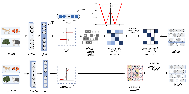
\includegraphics[width=0.95\linewidth]{papers_img/comparision_D2H_final.pdf}
    \caption{Comparison between deep learning for hashing and classification.}
    \label{Fig:comparison_classification_vs_hash}
        \vspace{-3ex}
\end{figure}

\subsection{Related Work}
\label{Section: related work}
\begin{table}[t]
    \centering
    \caption{Comparison of optimization and convergence guarantee of deep hashing methods.}
    \label{Table: summary of deep hashing algorithms}
    \resizebox{\linewidth}{!}{
\begin{tabular}{cccccc}
\toprule
\textbf{Type} & \textbf{Method} & \textbf{Model} 
  & \textbf{Quantization Loss} & \textbf{Optimization} & \textbf{Complexity} \\
\midrule
    \multirow{4}{*}{\centering Discrete} 
    & DDSH \cite{liDeepSupervisedHashing} & $\min L_s(\bb) + Q(\bu, \bb)$ & \centering $\|\cdot\|^2$ & BQP & \multirow{14}{*}{\centering ---} \\
    \cmidrule(lr){2-5}
    & DSDH \cite{li2017deep}& \multirow{3}{*}{\centering $\min L_s(\bu) + Q(\bu, \bb)$} & \multirow{3}{*}{\centering $\|\cdot\|^2$} & $sgn$ update &  \\ 
    & DPSH \cite{liFeatureLearningBased2016} & &  & DCC &  \\ 
    & DSARH \cite{zhang2026dsarh} & & & DCC + PGD-based AT &  \\
    \cmidrule(lr){1-5}
    \multirow{10}{*}{\centering Continuous}
    & DCH \cite{caoDeepCauchyHashing2018} &\multirow{4}{*}{\centering $\min L_s(\bu) + h(\bu)$} & $\log \left( 1 + \frac{\text{dist}_{\text{h}}(|\bu|, \mathbf{1})}{\gamma} \right)$ & \multirow{4}{*}{\centering SGDM} &  \\
    & DNNH \cite{laiSimultaneousFeatureLearning2015} & & $\mathcal{I}_{[-1,1]^d}(\bu)$ & &  \\
    & DSH \cite{liuDeepSupervisedHashing} & & $\| | \bu| - \mathbf{1}\|_1$ &  &  \\ 
    & DTSH \cite{wang2016DTSH} & & $\| | \bu| - \mathbf{1}\|_2^2$ &  &  \\ 
    & DHN \cite{zhuDeepHashingNetwork2016} & & $\sum_i\log(\cosh(|u_i|-1))$&  &  \\ 
    \cmidrule(lr){2-5}
    & MDSHC \cite{wang2023deep} & \scriptsize $\min L_c(\bu) + L_s (\bu)+ h(\bu)$ & $\| | \bu| - \mathbf{1}\|_1$ & RMSProp &  \\ 
    \cmidrule(lr){2-5}
    & HashNet \cite{Cao2017HashNetDL} & \multirow{2}{*}{\centering $\min L_s(\bu)$} & \multirow{2}{*}{\centering -} & SGDM &  \\     
    & OrthoHash \cite{hoeOneLossAll2021} & & & Adam &  \\
    % \cmidrule(lr){2-5}
    % & SBPG \cite{wang2024bregman} & \scriptsize $\min L_s(\bu) + h(\bu)$ & Weakly convex $h$ & SBregman PG & $\mathcal{O}(\varepsilon^{-4})$ \\
    \cmidrule(lr){2-6}
   & \textbf{DualHash-StoM} & \multirow{2}{*}{\small $ \min L_s(\bu) + Q(\bu,\bb) + h(\bb)$} & \multirow{2}{*}{$\| | \bb| - \mathbf{1}\|_1$} & \multirow{2}{*}{Sto Primal-Dual} & $\mathcal{O}(\varepsilon^{-4})$ \\
    & \textbf{DualHash-StoRM} & & & & $\mathcal{O}(\varepsilon^{-3})$ \\
    \bottomrule
    \end{tabular}
    }
    % \vspace{-5pt}
    \parbox{\linewidth}{\scriptsize
    \textbf{Notes}: 
    The \textbf{Type} column indicates whether binary codes are explicitly updated; DSARH is grouped with Discrete because its unified-hashing branch uses DCC updates.
    The \textbf{Model} column shows the core optimization objective, where \(\bb\) denotes binary codes and \(\bu\) denotes continuous outputs. The \textbf{Quantization Loss} column specifies the loss (\(Q(\cdot, \cdot)\) or \(h(\cdot)\)) for quantization error, with `-' indicating no explicit loss. 
    % The \textbf{Optimization} column describes the training strategy, with discrete methods focusing on binary code updates. 
    DCC stands for Discrete Cyclic Coordinate, PGD-based AT for projected-gradient adversarial training, while BQP denotes Binary Quadratic Programming. The \textbf{Complexity} column reports the convergence rate, with `-' indicating no such analysis.
    }
     \vspace{-2ex}
\end{table}
\paragraph{Optimization in Deep Hashing}
% Existing approaches to bridging the continuous--discrete gap in deep hashing fall into three categories.
% One line of work adopts continuous relaxation and introduces explicit quantization regularization on network outputs; in particular, W-type regularizers such as $\||\bz|-\mathbf{1}\|_1$ have been widely used to encourage binary-like activations \cite{liuDeepSupervisedHashing,wang2023deep,zhuDeepHashingNetwork2016}. Another line refines the discretization objective through greedy coding schemes, central similarity targets, or proxy-based supervision \cite{su2018greedy,yuanCentralSimilarityQuantization2020,semanticHashCenters2025}. Alternative strategies directly address binary constraints by introducing auxiliary hash codes \cite{liDeepSupervisedHashing,li2017deep,liFeatureLearningBased2016}. Notably, even recent architectures retain W-type regularization; for instance, He and Wei \cite{he2025mambahash} employ $\||\bz|-\mathbf{1}\|_2^2$ as a smooth surrogate for $\||\bz|-\mathbf{1}\|_1$ to facilitate gradient-based optimization. These developments indicate that the practical relevance of W-type regularization has not diminished. The remaining challenge is to develop theoretically grounded optimization methods that can directly handle nonsmooth W-type regularization under nonlinear deep network mappings, which is precisely the focus of this work.
% Recent studies have further strengthened backbone architectures to improve feature quality, extending deep hashing from conventional CNNs to hybrid CNN--Transformer frameworks \cite{he2024hybridhash}, Transformer-based hashing models \cite{chen2021transhash,wu2025fth,liu2025capmh}, and state-space architectures \cite{he2025mambahash}. 
W-type regularizers such as \blue{$\bz\mapsto\lVert|\bz|-\mathbf{1}\rVert_1$} have been 
widely adopted in deep hashing to bridge the gap between continuous 
network outputs and discrete binary codes~\cite{liuDeepSupervisedHashing,
wang2023deep,zhuDeepHashingNetwork2016}.
Alternative strategies either introduce auxiliary hash codes with a 
smoother surrogate $\|\cdot\|_2^2$~\cite{liDeepSupervisedHashing,
li2017deep,liFeatureLearningBased2016}, or refine the discretization 
objective via greedy coding, central similarity targets, or proxy-based 
supervision~\cite{su2018greedy,yuanCentralSimilarityQuantization2020,
semanticHashCenters2025}. Nevertheless, even recent architectures continue to rely on W-type regularization to mitigate quantization error. For instance,
He and Wei~\cite{he2025mambahash} employ \blue{$\bz\mapsto\lVert|\bz|-\mathbf{1}\rVert_2^2$}
as a smooth surrogate for \blue{$\bz\mapsto\lVert|\bz|-\mathbf{1}\rVert_1$} to ease
gradient-based optimization, highlighting that the core difficulty of
developing theoretically grounded methods for nonsmooth W-type
regularization under nonlinear network mappings has not been resolved.
This is precisely the gap this work aims to fill.

\paragraph{Primal-Dual and Stochastic Splitting Methods} Primal-dual methods, such as PDHG~\cite{chambolleFirstOrderPrimalDualAlgorithm2011} and its unified extensions~\cite{esserZhangChan2010}, are foundational tools for composite optimization with broad applications in imaging sciences. These methods enjoy ergodic $\mathcal{O}(1/k)$ convergence and remain stable under adjoint mismatch~\cite{chouzenouxAdjointMismatch}. For convex nonlinear saddle-point models, Gao and Zhang~\cite{gao2023alternative} proposed an alternative extrapolation scheme with provable convergence guarantees. Stochastic counterparts, notably SPDHG~\cite{chambolleSPDHG2018} \blue{and stochastic majorization-minimization subspace methods~\cite{chouzenouxStochasticMM2017}}, handle structured finite-sum objectives with almost-sure and ergodic convergence. In the nonconvex setting, Clason et al.~\cite{clasonAccelerationGlobalConvergence2019} established global convergence under the Kurdyka--{\L}ojasiewicz (KL) condition, while Guo et al.~\cite{guo2023preconditioned} further addressed nonconvex stochastic composite problems. More recently, Shumaylov et al.~\cite{shumaylovweakly} incorporated weakly convex neural-network regularizers into a primal-dual framework and proved convergence of PDHGM to critical points under the KL condition. When the problem admits a block-separable structure, splitting methods such as ADMM with its stochastic variants~\cite{wangGlobalConvergenceADMM2018,ADMMNolinear2024,chen2025convergence,bian2021stochastic} and stochastic alternative minimization~\cite{driggs2021stochastic,InertialProximalAlternating,bian2026stochastic} provide promising approaches for nonconvex multi-block optimization.

\paragraph{Stochastic Nonconvex Constrained Optimization}
From a constrained optimization perspective, Problem~\eqref{Eq: the general nonlinear composite problem in intro} \blue{can be reformulated via a variable lifting technique~\cite{wang2025augmentedrnn,jin2025multicomposite} as a nonlinearly constrained optimization problem of the form
\begin{equation}
  \label{Eq: the constrained reformulation}
  \min_{\bw}\; f(\bw) + h(\bw)
  \quad \text{s.t.}\quad
  \bc(\bw) = 0.
\end{equation}}Several recent works have established oracle complexity results for first-order stochastic augmented-Lagrangian and penalty methods for problems of this type. For instance, Jin and Wang \cite{jin2022stochastic} proposed a single-loop stochastic primal-dual method based on a linearized augmented-Lagrangian function, achieving oracle complexities of $\mathcal{O}(\varepsilon^{-6})$ from an arbitrary initial point and $\mathcal{O}(\varepsilon^{-5})$ from a feasible one for locating an $\varepsilon$-KKT point. By incorporating the recursive momentum estimator of \cite{cutkoskyMomentumBasedVarianceReduction2019}, Shi et al. \cite{shi2025momentum} developed a momentum-based linearized augmented-Lagrangian method, improving these bounds to $\mathcal{O}(\varepsilon^{-4})$, or the nearly optimal $\mathcal{O}(\varepsilon^{-3})$ when initialized at a nearly feasible point. To certify a stronger notion of stationarity that deterministically enforces constraint violation of at most $\varepsilon$, Lu et al. \cite{lu2024variancereducedfirstordermethodsdeterministically} introduced a linearized quadratic-penalty method with truncated momentum. Under a regularity condition on the constraint gradients, recursive momentum yields the nearly optimal complexity $\widetilde{\mathcal{O}}(\varepsilon^{-3})$. 

\noindent\textbf{Notations.} We use $a$, $\ba$, and $\bA$ to denote scalars, vectors, and matrices, respectively.
\blue{All vectors are column vectors. For $\bB\in\RR^{n\times d}$, we write $\bB=[\bb_1^\top;\dots;\bb_n^\top]$, where $\bb_i\in\RR^d$ and $\bb_i^\top$ is the $i$-th row of $\bB$. The same convention applies to iterates: $\bB^k=[(\bb_1^k)^\top;\dots;(\bb_n^k)^\top]$.}
Throughout this paper, \blue{$\bm{1}$ denotes an all-ones vector or matrix of the appropriate size}, and $i, j$ serve as indices. For matrix variables \(\bB\), \(\bY\), and \(\bLmbd\), we work directly in \(\RR^{n \times d}\), equipped with the Frobenius inner product \(\langle \cdot, \cdot \rangle\) and induced Frobenius norm \(\| \cdot \| := \sqrt{\langle \cdot, \cdot \rangle}\). Unless specified otherwise, \(\| \cdot \|\) denotes the Euclidean norm for vectors and the Frobenius norm for matrices. \( |\cdot| \) denotes element-wise absolute value. \blue{For a matrix $\bA=[A_{ij}]$, $\|\bA\|_1:=\sum_{i,j}|A_{ij}|$ denotes the entrywise $\ell_1$ norm.} For a closed set \(\calC \subseteq \RR^{q}\), the distance from a point \(\bx \in \RR^{q}\) to \(\calC\) is defined as \(\text{dist}(\bx, \mathcal{C}) := \min_{\by \in \mathcal{C}}\|\bx - \by\|\).
\blue{For simplicity, we use the same symbols $h$ and $h^*$ for their scalar forms and their separable extensions to vectors and matrices whenever no confusion can arise. The Fenchel conjugate of $h$~\cite{Rockafellar1998VariationalA} is $h^*(\bLmbd) := \sup_{\bZ \in \RR^{n\times d}} \{ \langle \bLmbd, \bZ \rangle - h(\bZ) \}$ for $\bLmbd \in \RR^{n\times d}$.}

\section{Preliminary}
The extended real-valued function $f: \mathbb{R}^{q}\rightarrow (-\infty, +\infty]$ is called \textit{proper} if its domain $\text{dom}(f) := \{\bx \in \RR^q\mid f(\bx) < +\infty\}$ is nonempty and $\inf\limits_{\bx \in \mathbb{R}^q}f > -\infty$; \blue{it is called \textit{lower semicontinuous} if its epigraph $\text{epi}(f) := \left\{ (\bx, t) \in \mathbb{R}^{q+1}\mid f(\bx) \leq t \right\}$ is closed.}
For a proper, \blue{lower semicontinuous}, and convex function $f$, the \textit{proximal mapping} of $f$, denoted by $\operatorname{prox}_{\tau f}(\by)$, is defined as
\begin{align}
    % \label{Def: the definition of proximal operator}
    \operatorname{prox}_{\tau f}(\by) := \argmin\limits_{\bx \in \operatorname{dom}(f)}\left\{ f(\bx) + \frac{1}{2\tau}\|\bx - \by\|^{2}\right\}, \notag
\end{align} 
where $\tau$ is a positive scalar parameter. The proximal mapping admits the following
properties.
\begin{proposition}\label{prop:rockafellar}
\textnormal{\cite{Rockafellar1998VariationalA}}
    Let $f : \mathbb{R}^{q}\rightarrow \mathbb{R}\cup \{+\infty\}$ be proper and
    \blue{lower semicontinuous}. Then, the following holds.
    \begin{enumerate}[label=(\roman*)]
        \item The set $\operatorname{prox}_{\tau f}(\bx)$ is nonempty and compact
            for any $\bx \in \mathbb{R}^{q}$ and $\tau > 0$.

        \item If $f$ is convex, then $\operatorname{prox}_{\tau f}(\bx)$
            contains exactly one value for any $\bx \in \mathbb{R}^{q}$ and
            $\tau > 0$.
    \end{enumerate}
\end{proposition}

\blue{We use the StoRM (stochastic recursive momentum) variance-reduction estimator \cite{cutkoskyMomentumBasedVarianceReduction2019}. In the following generic stochastic notation, let $\phi(\bx) = \mathbb{E}_{\xi}[\phi(\bx;\xi)]$ with $\xi \in \Xi$; this notation is distinct from the finite-sum function $F(\bx,\bB)$ defined later for the split hashing model.} Standard momentum methods use
\begin{align*}
    \blue{\bg^{k} = \rho_{k}\nabla \phi(\bx^{k}, \xi^{k}) + (1 - \rho_{k}) \bg^{k-1}, \text{ where } \rho_{k}\in [0, 1],}
\end{align*}
\blue{yielding a biased estimate of $\nabla \phi(\bx^{k})$.}
\blue{StoRM adds the correction term $(1 - \rho_{k-1}) (\nabla \phi(\bx^{k}, \xi^{k}) - \nabla \phi(\bx^{k-1}, \xi^{k}))$, resulting in:}
\begin{align}
     \label{Eq: the generic StoRM estimator}\blue{\bg^{k}=\left\{\begin{array}{ll}\nabla \phi\left(\bx^{k}, \xi^{k}\right), & \text{if } k=1, \\ \nabla \phi\left(\bx^{k}, \xi^{k}\right) + \left(1-\rho_{k-1}\right)\left( \bg^{k-1} - \nabla \phi\left(\bx^{k-1}, \xi^{k}\right) \right), & \text{if } k>1,\end{array}\right.}
\end{align}
This estimator exploits the smoothness of $\blue{\phi}(\cdot, \xi)$, leading to efficient variance reduction. \blue{Here $\bg^{k}$ is the stochastic direction at iteration $k$, used in the generic update $\bx^{k+1}=\bx^{k}-\eta_{k}\bg^{k}$.} When $\rho_{k} = 1$, $\bg^{k}$ reduces to vanilla mini-batch SGD. We set $\rho_{k}\in (0,1)$ for $k \geq 1$ in this paper.

\blue{A differentiable} function $f: \RR^q \rightarrow \RR$ is said to be $L_f$-smooth if $\| \nabla f(\bx) - \nabla f(\bx') \| \leq L_f \| \bx - \bx'\|$ for all $\bx,\, \bx' \in \RR^q$.
A mapping $\mathcal{M} : \blue{\Omega} \to \RR^l$ is said to be $C$-Lipschitz continuous if $\|\mathcal{M}(\bx) - \mathcal{M}(\bx')\| \leq C\|\bx - \bx'\|$ for all $\bx, \bx' \in \blue{\Omega}$.
For an $L_f$-smooth function, the descent lemma \blue{\cite{Bertsekas1997}} states that
\begin{align}
% \label{Eq: the descent lemma}
    f(\bx) \leq f(\bx') + \langle \nabla f(\bx'), \bx - \bx' \rangle + \frac{L_f}{2} \| \bx - \bx'\|^2. \notag
\end{align}

% \section{Problem reformulation}
% \label{Section: Problem Reformulation}
% \subsection{W-type Regularized Deep Hashing Model}
% Deep hashing methods aim to learn network parameters \(\bx \in \RR^{d_{\bx}}\) to generate discrete codes that preserve semantic similarity effectively in the Hamming space. 
% A natural approach is to minimize a similarity-preserving loss function \( \frac{1}{n}\sum_{i=1}^n L_s(\text{sgn}(\bD_i(\bx)))\) where $n$ is the number of training samples, $\bD_i(\bx)$ represents the \(i\)-th network output and \(f_i\) is the similarity-preserving loss function (e.g., pairwise cross-entropy loss \cite{zhuDeepHashingNetwork2016}). However, the function \( sgn(\cdot) \) renders standard backpropagation infeasible due to its zero gradient for all nonzero inputs. This discreteness poses a central challenge in deep hashing.

% A W-type regularization (e.g., $\lambda | |z| - 1 |$) has effectively mitigated this issue. This type of regularization encourages outputs to approach binary values \(\{-1, 1\}\) during training. Specifically, the model is trained to produce continuous outputs \(\bu_i = \bD_i(\bx)\) with W-type regularization, and binary codes are obtained post-training via \(\bb_i = \text{sgn}(\bu_i)\).  Consequently, we formulate the core optimization problem for W-type regularized deep hashing methods as follows,
% \begin{align}
% \label{Eq: the primal deep hashing problem}
% \min_{\bx \in \RR^{d_{\bx}}} \quad \frac{1}{n} \sumn f_i (\bx) + \sumn h(\bD_i(\bx)), 
% \end{align}where \(\frac{1}{n}\sumn f_i\) is the similarity-preserving loss, \(D_i\) is the \(i\)-th network output and \(h\) is a W-type regularization.
% % \footnote{In the problem \eqref{Eq: the primal deep hashing problem}, we use vectorized \(\bz\), thus the regularization is also \(\| |\bz| - \bm{1}\|_1 = \sumn | |z_i| - 1 |\)}.
% \subsection{A Two-Block Structured Reformulation}
% We then employ variable splitting % \cite{wangLiftedBregmanTraining2022, zengBlockCoordinateDescent2018, lauProximalBlockCoordinate2018}, ]\
% to reformulate problem \eqref{Eq: the primal deep hashing problem} equivalently as the constrained problem:
% \begin{align} 
% \label{Eq: constrained_dlh} 
% \min_{\bx \in \RR^{d_{\bx}}, \bB \in \RR^{n\times d}}&\quad \frac{1}{n} \sumn f_i (\bx) + \sum_{i=1}^n h(\bb_i) \notag \\ 
% \text{s.t.} &\quad \bb_i = \bD_i(\bx), \; \forall i=1,\dots,n. 
% \end{align} Combined with the quadratic penalty method \cite{nocedal1999numerical}, this transformation yields the following two-block finite-sum optimization problem:
% \begin{align} 
% \label{Prop: block-wise regularized problem} 
% \nonumber&\min_{\bx \in \RR^{d_{\bx}}, \bB \in \RR^{n\times d}} J(\bx, \bB) \\
% &= \overbrace{\underbrace{\frac{1}{n}\sum_{i=1}^n f_i(\bx)}_{f(\bx)} + \underbrace{\frac{\gamma}{2n} \sum_{i=1}^n \| \bD_i(\bx) - \bb_i\|^2}_{P(\bx, \bB)}}^{F(\bx, \bB) = \frac{1}{n}\sumn F_i(\bx, \bb_i)} + \underbrace{\sum_{i=1}^n h(\bb_i)}_{h(\bB)}. \tag{P}
% \end{align} Here, \( \bB = [\bb_1, \bb_2, \dots, \bb_n]\) and \( \gamma > 0 \) is the penalty parameter. This reformulation decomposes the original problem \eqref{Eq: the primal deep hashing problem} into simpler structural blocks, enabling us to exploit the problem structure better. Building upon this problem, we develop a stochastic primal-dual algorithm that effectively addresses the challenges above.
\section{Problem Reformulation}
\label{Section: Problem Reformulation}
\subsection{W-type Regularization in Deep Hashing Model}
\label{Sec:W-type Regularized Deep Hashing Model}
Deep hashing aims to learn network parameters \(\bx \in \RR^{\blue{q}}\) that generate binary codes preserving semantic similarity in the Hamming space. A direct formulation is
\begin{align}
\label{Eq:direct_deep_hashing_problem}
\blue{\min_{\bx \in \RR^{q}}\ \frac{1}{n}\sum_{i=1}^{n}\ell_{s,i}\!\big(\operatorname{sgn}(\mathcal{D}(\bx))\big),}
\end{align}
where \(n\) is the number of training samples, \blue{\(\bD_i:\RR^q\to\RR^d\) is the continuous network output mapping for sample \(i\), and \(\ell_{s,i}:\RR^{n\times d}\to\RR\) is a similarity-preserving loss} (e.g., pairwise cross-entropy \cite{zhuDeepHashingNetwork2016}). This objective is hard to optimize by backpropagation because \(\operatorname{sgn}(\cdot)\) is nondifferentiable and has zero gradient almost everywhere. 

\blue{To address this issue, penalties whose graphs are W-shaped, vanishing exactly at
$\pm1$, are added to drive continuous outputs toward $\{-1,1\}^d$. They are standard in
deep hashing~\cite{liuDeepSupervisedHashing,wang2016DTSH,zhuDeepHashingNetwork2016,
yuanCentralSimilarityQuantization2020,he2025mambahash,yin2026crh}.
Related distance-based regularizers are also used to train binary and quantized
networks~\cite{yin2018binaryrelax,bai2019proxquant}. We formalize the scalar penalties
considered here as the W-type class in \Cref{def:wtype}.}

\begingroup
\color{blue}
\begin{definition}[W-type regularizer]\label{def:wtype}
Let \(\phi:\mathbb{R}\to[0,+\infty)\). For \(\bz\in\mathbb{R}^{d}\) and \(\bZ\in\mathbb{R}^{n\times d}\), define \(h(\bz):=\sum_{j=1}^{d}\phi(z_j)\) and \(h(\bZ):=\sum_{i=1}^{n}\sum_{j=1}^{d}\phi(z_{ij})\). We call \(h\) a \emph{W-type regularizer} if \(\phi\) satisfies:
\begin{enumerate}[label=\textup{(W\arabic*)}]
  \item\label{W1} \(\phi\) is even and continuous, and \(\phi(t)=0\) if and only if \(t\in\{-1,1\}\);
  \item\label{W2} \(\phi\) is convex on \([1,+\infty)\);
  \item\label{W3} \(\phi\) decreases at a nonvanishing rate on \([0,1)\): for every \(b\in(0,1)\) there exists \(c_b>0\) such that \(\phi(s)-\phi(t)\ge c_b(t-s)\) for all \(0\le s<t\le b\).
\end{enumerate}
\end{definition}



Each condition is used once: \ref{W1} makes the zero set of \(h\) exactly \(\{-1,1\}^{n\times d}\); \ref{W2} yields the envelope formula of Lemma~\ref{lem:wtype-conj}, so that the dual reformulation leaves \(h\) unchanged on \(|t|\ge1\); and \ref{W3} excludes stationary points in \((-1,1)\) (Lemma~\ref{lem:no-inner-stationary}), which gives the stationarity-to-contact implication of Proposition~\ref{prop:transfer}.

\begin{table}[t]
\centering
\color{blue}
\caption{Representative W-type regularizers, with \(\lambda,\delta>0\), \(\psi(u):=\frac12[(1+u)\log(1+u)+(1-u)\log(1-u)]\), and \(\operatorname{Hub}_{\delta}(s):=s^2/(2\delta)\) if \(|s|\le\delta\), \(|s|-\delta/2\) otherwise. Outside \(\operatorname{dom}\phi^*\), \(\phi^*=+\infty\); \(\operatorname{clip}\) denotes projection onto \([-\lambda,\lambda]\); ``---'' means that no closed form is available.}
\label{tab:wtype}
\resizebox{\linewidth}{!}{
\begin{tabular}{lllcccc}
\toprule
\multicolumn{2}{l}{\(\phi(t)\)} & Used in & \(\partial\phi(0)\) & \(\phi^*(y)\) & \(\operatorname{dom}\phi^*\) & \(\operatorname{prox}_{\sigma\phi^*}(v)\)\\
\midrule
\multirow{2}{*}{\(\lambda\bigl||t|-1\bigr|^{p}\)}
 & \(p=1\) & \cite{liuDeepSupervisedHashing,wang2023deep,bai2019proxquant}
 & \(\{\pm\lambda\}\) & \(|y|\) & \([-\lambda,\lambda]\)
 & \(\operatorname{clip}\bigl(\operatorname{sgn}(v)(|v|-\sigma)_+\bigr)\)\\
 & \(p=2\) & \cite{wang2016DTSH,he2025mambahash,semanticHashCenters2025,yin2026crh,bai2019proxquant}
 & \(\{\pm2\lambda\}\) & \(|y|+\frac{y^2}{4\lambda}\) & \(\mathbb{R}\)
 & \(\operatorname{sgn}(v)\frac{(|v|-\sigma)_+}{1+\sigma/(2\lambda)}\)\\
\midrule
\multicolumn{2}{l}{\(\lambda\log\cosh(|t|-1)\)} & \cite{zhuDeepHashingNetwork2016,yuanCentralSimilarityQuantization2020}
 & \(\{\pm\lambda\tanh1\}\)
 & \(|y|+\lambda\psi(|y|/\lambda)\)
 & \([-\lambda,\lambda]\) & ---\\
\multicolumn{2}{l}{\(\lambda\operatorname{Hub}_{\delta}(|t|-1)\)} & ---
 & \(\{\pm\lambda\min\{1,\frac1\delta\}\}\) & \(|y|+\frac{\delta y^2}{2\lambda}\) & \([-\lambda,\lambda]\)
 & \(\operatorname{clip}\Bigl(\operatorname{sgn}(v)\frac{(|v|-\sigma)_+}{1+\sigma\delta/\lambda}\Bigr)\)\\
\bottomrule
\end{tabular}}
\end{table}

All rows of Table~\ref{tab:wtype} satisfy \ref{W1}--\ref{W3}, and none is differentiable at \(0\): its subdifferential there is \(\{\pm c\}\) with \(c>0\). This is forced by the class itself, since an even \(\phi\) that is differentiable at \(0\) has \(\phi'(0)=0\), contradicting \ref{W3}. The rows differ in where else they are nonsmooth and how fast they grow. For \(p=1\) the kinks also lie at \(\pm1\), where the binary codes are. The other three rows are smooth at \(\pm1\), but the kink at \(0\) still rules out \(L\)-smoothness and weak convexity, so standard complexity guarantees for gradient methods do not apply to them either. Tail growth determines \(\operatorname{dom}\phi^*\): smoothing \(p=1\) by squaring gives \(\operatorname{dom}\phi^*=\mathbb{R}\), whereas smoothing it by \(\log\cosh\) or \(\operatorname{Hub}_\delta\) keeps \(\operatorname{dom}\phi^*=[-\lambda,\lambda]\).

\setcounter{lemma}{1}
\begin{lemma}\label{lem:wtype-conj}
Let \(h\) be a W-type regularizer. Then \(\phi^*\) is proper, lower semicontinuous, convex, and even, \(\phi^*(y)\ge|y|\) for all \(y\), and \(\operatorname{dom}\phi^*\) has nonempty interior. Moreover,
\[
  \phi^{**}(t)=\phi\bigl(\max\{|t|,1\}\bigr),\qquad
  \phi^{**}(t)=\phi(t)\iff |t|\ge1.
\]
Consequently, \(h^*(\bLmbd)=\sum_{i,j}\phi^*(\Lambda_{ij})\), \(h^{**}(\bB)=\sum_{i,j}\phi^{**}(b_{ij})\), and \(h(\bB)=h^{**}(\bB)\) if and only if \(|b_{ij}|\ge1\) for all \(i,j\).
\end{lemma}
\begin{proof}
Let \(\psi(t):=\phi(\max\{|t|,1\})\). By \ref{W1}--\ref{W2}, \(\phi\) is convex and nonnegative on \([1,+\infty)\), with \(\phi(1)=0\); hence it is nondecreasing there. Thus \(s\mapsto\phi(\max\{s,1\})\) is convex and nondecreasing on \([0,+\infty)\), so \(\psi\) is convex and satisfies \(\psi\le\phi\). Conversely, any convex \(q\le\phi\) satisfies \(q(\pm1)\le0\), hence \(q\le0=\psi\) on \([-1,1]\), while \(q\le\phi=\psi\) on \(|t|\ge1\). Therefore \(\phi^{**}=\psi\), the largest lower semicontinuous convex minorant of \(\phi\)~\cite[Theorem~12.2]{rockafellar1970convex}. For \(|t|<1\), \ref{W1} gives \(\phi(t)>0=\psi(t)\), proving the contact-set formula.

Evaluating the definition of \(\phi^*\) at \(t=\pm1\) gives \(\phi^*(y)\ge|y|\). Since \(\phi(t_0)>0\) for any \(t_0>1\), convexity on \([1,+\infty)\) implies at least linear growth for large \(t\); evenness gives the same for negative \(t\). Hence \(\operatorname{dom}\phi^*\) contains an open interval around zero. The separable formulas follow from~\cite[Theorem~16.4]{rockafellar1970convex}.
\end{proof}

\begin{remark}[Scope of Definition~\ref{def:wtype}]\label{rem:wtype-scope}
Conditions \ref{W2} and \ref{W3} cannot be dropped.
\begin{enumerate}[label=\textup{(\roman*)}]
  \item \emph{Without \ref{W3}.} The function \(\phi(t)=|t^2-1|\) satisfies \ref{W1}--\ref{W2} but violates \ref{W3}, because its slope vanishes at \(0\); indeed \(\partial\phi(0)=\{0\}\). In the setting of Example~\ref{ex:gap}, its convex envelope is \(\phi^{**}(t)=(t^2-1)_+\), and \((b,\Lambda)=(0,0)\) satisfies the KKT conditions. It is also stationary for Problem~(P), but \(J(b)=1-\tfrac12b^2\) near zero, so it is a local maximizer. Here \(|b|<1\) and \(h(0)\ne h^{**}(0)\), showing why \ref{W3} is needed for Proposition~\ref{prop:transfer}.
  \item \emph{Without \ref{W2}.} The function \(\phi(t)=\lambda\log\bigl(1+\bigl||t|-1\bigr|\bigr)\) satisfies \ref{W1} and \ref{W3}, but its tails are concave. Its sublinear growth gives \(\operatorname{dom}\phi^*=\{0\}\) and \(h^{**}\equiv0\), so the dual reformulation forces \(\bLmbd=\zero\) and removes the regularizer.
\end{enumerate}
Finally, the row \(p=2\) of Table~\ref{tab:wtype} satisfies \ref{W1}--\ref{W3}, so the structural optimality propositions remain valid for it. Its conjugate has full domain, however, and the current complexity analysis, which uses boundedness of the dual domain, does not cover this quadratic-growth case. Condition~\ref{W1} specifies the binary-code zero set and is therefore part of the model definition.
\end{remark}
\endgroup
Specifically, the model is trained to produce the \(i\)-th continuous network output \(\bD_i(\bx)\) with W-type regularization \(h\), and binary codes are obtained post-training via \(\operatorname{sgn}(\bD_i(\bx))\blue{\in\{-1,1\}^d}\). \blue{Consequently, we formulate the following core optimization problem for W-type regularized deep hashing methods, which serves as a continuous surrogate of Problem~\eqref{Eq:direct_deep_hashing_problem}:}
\begin{align}
\label{Eq: the primal deep hashing problem}
\min_{\bx \in \RR^{\blue{q}}} \quad \frac{1}{n}\sum_{i=1}^n f_i(\bx) + \sum_{i=1}^n h(\bD_i(\bx)),
\tag{P0}
\end{align}\blue{where
\(f_i(\bx):=\ell_{s,i}\!\left(\mathcal{D}(\bx)\right)+\frac{\mu}{2}\|\bx\|^2\) with \(\mu>0\) ensures coercivity.}

We then employ variable splitting by introducing \blue{continuous auxiliary variables \(\bb_i\in\RR^d\) and \(\bB=[\bb_1^\top;\ldots;\bb_n^\top]\in\RR^{n\times d}\), subject to \(\bb_i=\bD_i(\bx)\) for all \(i=1,\dots,n\),} which yields the following equivalent nonlinearly constrained problem:
\begin{align}
    \blue{\min_{\bx \in \RR^{q},\ \bB \in \RR^{n\times d}}\quad \frac{1}{n}\sum_{i=1}^{n} f_i(\bx)+\sum_{i=1}^{n}h(\bb_i)\quad \text{s.t.}\quad \bb_i=\bD_i(\bx),\ \forall i=1,\dots,n.} \notag
\end{align}
We then \blue{relax these constraints by} the quadratic penalty method \cite[Sec.~17.1]{nocedalWright2006} to obtain the following two-block finite-sum optimization problem:
\begin{align}
    \label{Prop: block-wise regularized problem}
    \blue{\min_{\bx \in \RR^{q},\,\bB \in \RR^{n\times d}}\ J(\bx,\bB):=F(\bx,\bB)+h(\bB),} \tag{P}
\end{align}
\blue{Here, \(\gamma>0\) is the penalty parameter, and we use the separable extension \(h(\bB):=\sum_{i=1}^{n}h(\bb_i)\) for matrices. We define}
\begin{align}
    \blue{F(\bx,\bB)} &\blue{:= \frac{1}{n}\sum_{i=1}^{n}F_i(\bx,\bb_i),} \notag\\
    \blue{F_i(\bx,\bb_i)} &\blue{:= f_i(\bx)+\frac{\gamma}{2}\|\bD_i(\bx)-\bb_i\|^2,} \notag
\end{align}
\blue{Averaging over \(i\) gives the decomposition \(F=f+P\), where}
\begin{align}
    \blue{f(\bx)} &\blue{:= \frac{1}{n}\sum_{i=1}^{n}f_i(\bx),} \notag\\
    \blue{P(\bx,\bB)} &\blue{:= \frac{\gamma}{2n}\sum_{i=1}^{n}\|\bD_i(\bx)-\bb_i\|^2.} \notag
\end{align}
This reformulation decomposes the original problem \eqref{Eq: the primal deep hashing problem} into simpler structural blocks, enabling us to exploit the problem structure better. Building upon Problem~\eqref{Prop: block-wise regularized problem}, we develop a stochastic primal-dual algorithm {that addresses the lack of tractable proximal mappings in the nonsmooth composite form and the absence of convergence guarantees in existing deep hashing methods.}

\section{\blue{Primal--Dual Formulation and Optimality Guarantees}}
\label{Section: Methodology}
% \subsection{DualHash: A Stochastic Primal-Dual Hashing Algorithm}
% Inspired by PDHG \cite{chambolleFirstOrderPrimalDualAlgorithm2011} in convex optimization and its nonconvex extension PPDG \cite{guoPreconditionedPrimalDualGradient2023}, we consider the equivalent constrained formulation of  the problem \eqref{Prop: block-wise regularized problem}:
% \begin{align}
% \min_{\bx \in \RR^{d_{\bx}}, \bB \in \RR^{n\times d}, \by \in \RR^{n\times d}} &\quad F(\bx, \bB) + h(\bY) \notag \\
% \text{s.t. } &\quad \bY = \bB \nonumber ,
% \end{align} whose corresponding dual problem is
% \begin{align}
% \label{Prop: the dual problem}
% \max_{\bLmbd \in \RR^{n\times d}} \min_{\bx \in \RR^{d_{\bx}}, \bB \in \RR^{n\times d}, \by \in \RR^{n\times d}} &\quad F(\bx, \bB) + h(\bY) + \langle \bLmbd, \bB - \bY \rangle. \tag{D}
% \end{align}
% Recalling the definition of the conjugate function \cite{Rockafellar1998VariationalA}:
% \begin{equation}
% \label{eq:fenchel_conjugate}
% h^*(\bY) := \sup_{\bx \in \RR^{n\times d}} \{ \langle \bY, \bx \rangle - h(\bx) \}, \quad \bY \in \RR^{n\times d}
% \end{equation} and observing that the minimization with respect to $\bY$ in the problem \eqref{Prop: the dual problem} can be performed independently, we then simplify the Lagrangian function in the problem \eqref{Prop: the dual problem} to
% \begin{align}
% \label{Eq: simplified_lagrangian}
% \calL(\bx, \bB, \bLmbd) := F(\bx, \bB) + \langle \bB, \bLmbd \rangle - h^*(\bLmbd).\tag{\(\calL\)}
% \end{align}

% Through this transformation, we replace $h(\bY)$ with $-h^*(\bLmbd)$ and can optimize \(h^*\) in the dual space. Since $h^*$ is always convex and l.s.c. \cite{Rockafellar1998VariationalA}, it means that the $\text{prox}_{h^*}(\cdot)$ is often much easier to compute (potentially having a closed-form solution) than that of $h$.  For $h(\bz) = \sum_{i=1}^n \lambda ||z_i| - 1|$, we derive its conjugate function as illustrated in \Cref{fig:w_type_regularization}:
% \begin{align*}
% &h^*(\bx) = \sum_{i=1}^n h^*(x_i),\,\, \notag \\
% & \text{where } h^*(x_i) = \begin{cases}
%     |x_i|, & \text{if } x_i \in [-\lambda, \lambda],\\
%     +\infty, & \text{otherwise},
%     \end{cases}
% \end{align*} whose proximal operator  in the piecewise solution is
% \begin{align}
%     \label{Eq: the proximal mapping of conjugate function}
%     [\operatorname{prox}_{\tau h^*}(\by)]_i =
%     \begin{cases}
%         \lambda, & y_i > \lambda +\tau,\\
%         y_i -\tau, & \tau < y_i \leq \lambda +\tau, \\
%         0, & -\tau \leq y_i \leq\tau, \\
%         y_i +\tau, &  - \lambda -\tau \leq y_i < -\tau, \\
%         -\lambda, & y_i < -\lambda -\tau.
%     \end{cases}
% \end{align} This motivates us to perform a proximal step to update \(\bLmbd\).
% \begin{figure}[!t]
% \centering
% \includegraphics[width=\columnwidth]{papers_img/W_type_with_its_conjugate_func.pdf}
% \caption{W-type regularization function $h(z) = \lambda ||z| - 1|$ and its conjugate function $h^*(x)$.}
% \label{fig:w_type_regularization}
% \vspace{-1ex}
% \end{figure} We now outline \textbf{DualHash}, which employs an alternating update scheme for $\bx, \bB, \bm{\Lambda}$.
% we adopt a stochastic first-order method for the $\bx$-update since computing the full gradient \( \nabla_{\bx} F(\bx, \bB) \) is computationally expensive for typically the large number of samples $n$ in deep learning. Specifically, at each iteration $k$, we uniformly sample a mini-batch \(\calJ_k \subseteq \{1,\cdots,n\}\) with \(b_k = |\calJ_k| \leq n\) and compute:
% \begin{align}
% \label{Eq: the mini batch stochastic gradient estimator of F at x}
% \nabla_{\bx} F(\bx^k, \bB^k; \calJ_k)
% =\, \frac{1}{|\mathcal{J}_k|}\sum_{j \in \mathcal{J}_k} \nabla_{\bx} F_j(\bx^k, \bb_j^k).
% \end{align}
% Then we utilize this approximation within an optimization strategy chosen to enhance efficiency (e.g., incorporating momentum or variance reduction), as detailed in \Cref{Sec: Algorithm implementations}.
% Second, the auxiliary variable $\bB$ is updated via a simple gradient descent step \eqref{Eq: the update of B}; this suffices because the objective \eqref{Eq: simplified_lagrangian} with respect to $\bB$ is smooth with an inexpensive gradient,
% % which is slightly different from \cite{chambolleFirstOrderPrimalDualAlgorithm2011}:
%     \begin{align}
%    \nonumber \bB^{k+1} &= \bB^k - \tau \nabla_{\bB}\calL(\bx^{k+1}, \bB^k, \bLmbd^k)\\
%     &= \bB^k - \tau \left( \nabla_{\bB} F(\bx^{k+1}, \bB^k) + \bLmbd^k \right). \label{Eq: the update of B}
%     \end{align}
%     Finally, the dual variable $\bLmbd$ is updated via proximal gradient ascent on $h^*$, using an extrapolation step introduced in \cite{chambolleFirstOrderPrimalDualAlgorithm2011}. The update solves the following optimization problem:
% \begin{align}
%     \bLmbd^{k+1} &= \text{prox}_{(1/\tau h^*)} \left( \bLmbd^k + \left(2\bB^{k+1} - \bB^k  \right) \right) \notag \\
%     &=  \arg\min_{\bLmbd \in \RR^{n\times d} } \left\{ h^*(\bLmbd) - \langle \bLmbd, 2\bB^{k+1} - \bB^k \rangle \right. \notag \\
%     &\quad\quad\quad\quad\quad\quad\quad\quad\quad\quad\left. + \frac{\tau}{2} \| \bLmbd - \bLmbd^k\|^2 \right\}.
%     \label{Eq: the update of lambda}
% \end{align}
% \subsection{Implementations}
% \label{Sec: Algorithm implementations}
% The unified DualHash framework allows for flexible choices in the $\bx$ update step based on a mini-batch stochastic gradient approximation \eqref{Eq: the mini batch stochastic gradient estimator of F at x}. This flexibility enables us to incorporate advanced stochastic optimization techniques. We thus instantiate the $\bx$-update using two well-established approaches: \textbf{momentum} \cite{Nesterov1983AMF, Polyak1964} and \textbf{variance reduction} \cite{driggs2022biased}, which can improve empirical training efficiency and can also improve the theoretical convergence guarantees \cite{Liu2020AnIA,sutskever2013importance}.

% % \vspace{5pt}
% \paragraph{DualHash-StoM}
% %Numerically,
% The heavy ball method \cite{Polyak1964} and Nesterov acceleration \cite{Nesterov1983AMF} can be integrated with stochastic gradient descent (SGD) to yield accelerated variants like SGD with momentum, which significantly speeds up convergence.
% This approach has become a popular strategy for training neural networks \cite{fotopoulos2024review,Hertrich2020InertialSP}. We thus incorporate this technique and compute the stochastic gradient estimator (Line 3 of \Cref{alg:our_algorithm_sgdm}) as:
% \begin{align}
% \label{Eq: the stochastic approximate in SGDM}
%     \bG^k = \nabla_{\bx} F(\bz^k, \bB^k; \calJ_k),\, \text{where } \bz^k = \bx^k + \beta_k (\bx^k - \bx^{k-1}).
% \end{align} The update of \( \bx^k\) (Line 4 of Alg. \ref{alg:our_algorithm_sgdm}) is then:
% \begin{align}
% \label{Eq: the update of x in SGDM}
%     \bx^{k+1} = \by^k - \eta_k \bG^k,\,\text{where } \by^k = \bx^k + \alpha_k (\bx^k - \bx^{k-1}).
% \end{align} The overall algorithm, DualHash-StoM, is detailed in \Cref{alg:our_algorithm_sgdm}.
% \begin{remark}
% The momentum acceleration framework in \eqref{Eq: the update of x in SGDM} covers these two accelerations:
% Nesterov acceleration \cite{Nesterov1983AMF} corresponds to $\alpha_k = \beta_k \neq 0$; the heavy-ball method \cite{Polyak1964} is obtained with $\beta_k = 0$; vanilla SGD is recovered when $\alpha_k = \beta_k = 0$; In this paper, we set $\alpha_k, \beta_k \in (0,1)$ for all $k \geq 1$.
% \end{remark}

% % \vspace{3pt}
% \paragraph{DualHash-StoRM}
% Alternatively, we employ the STORM estimator \cite{cutkoskyMomentumBasedVarianceReduction2019} for the $\bx$-update. STORM utilizes a recursive momentum mechanism to reduce gradient variance, which is motivated by SGDM. Unlike some other variance reduction techniques (e.g., SVRG \cite{johnsonAcceleratingStochasticGradient2013}, SARAH \cite{SARAH2017}) that require full-gradient or large-batch gradient computations, STORM achieves variance reduction without such requirements. Given its practical effectiveness in deep learning \cite{cutkoskyMomentumBasedVarianceReduction2019,levy2021storm+}, we compute the stochastic gradient estimator (Line 3 of \Cref{alg:our_algorithm_storm}) as:
% % {\small
% % \begin{align}
% % \label{Eq: the stochastic approximate in STORM}
% % \bD^k =
% % \begin{cases}
% % \nabla_{\bx} F(\bx^1, \bB^1; \calJ_1), & \text{if } k = 1, \\
% % \nabla_{\bx} F(\bx^k, \bB^k; \calJ_k) + (1 - \rho_{k-1}) \left( \bD^{k-1} - \nabla_{\bx} F(\bx^{k-1}, \bB^{k-1};\calJ_{k-1})\right), & \text{if }k > 1.
% % \end{cases}
% % \end{align}}
% {\small
% \begin{align}
% \label{Eq: the stochastic approximate in STORM}
% \bD^k =
% \begin{cases}
% \nabla_{\bx} F(\bx^1, \bB^1; \mathcal{J}_1), &\text{if }  k = 1, \\
% (1 - \rho_{k-1}) \big( \bD^{k-1} - \nabla_{\bx} F(\bx^{k-1}, \bB^{k-1};\mathcal{J}_{k-1})\big)\\
% +\nabla_{\bx} F(\bx^k, \bB^k; \mathcal{J}_k), & \text{if } k > 1.
% \end{cases}
% \end{align}}
% The update of $\bx$ (Line 4 of \Cref{alg:our_algorithm_storm}) is then
% \begin{align}
% \label{Eq: the update of x in STORM}
%     \bx^{k+1} = \bx^k - \eta_k \bD^k.
% \end{align} The overall algorithm, DualHash-StoRM, is detailed in \Cref{alg:our_algorithm_storm}.

% \begin{figure}[!htbp]
%     \vspace{-5mm}
%     \begin{minipage}[t]{0.485\textwidth}
%         \begin{algorithm}[H]
%        \caption{DualHash-StoM}
%         \small   % 或使用 \footnotesize 更小
%         \setlength{\baselineskip}{0.8\baselineskip}  % 减少行间
%       \label{alg:our_algorithm_sgdm}
%       \begin{algorithmic}[1]
%         \STATE \textbf{Initialize:} $\bx^1 = \bz^1 = \by^1 \in \RR^{d_{\bx}} $, \( \bB^1 \in \RR^{n\times d},\, \bLmbd^1\in \RR^{n\times d}\), parameters $\{\eta_k\} $, $\tau$, $b_k$, $\{\alpha_k, \beta_k \in (0,1)\}$
%         \FOR{$k = 1, 2, \ldots$}
%           \STATE Compute \(\bG^k\) by \eqref{Eq: the stochastic approximate in SGDM}
%           \STATE Update $\bx^{k+1}$ by \eqref{Eq: the update of x in SGDM}
%           \STATE Update $\bB^{k+1}$ by \eqref{Eq: the update of B}
%           \STATE Update $\bm{\Lambda}^{k+1}$ by \eqref{Eq: the update of lambda}
%         \ENDFOR
%         \STATE \textbf{Return:} $\bx_R$ where \blue{$R$ is uniformly sampled from $\{1, \ldots, T\}$}
%       \end{algorithmic}
%     \end{algorithm}
%   \end{minipage}
%   \hspace{0.5mm}
%   \begin{minipage}[t]{0.485\textwidth}
%     \begin{algorithm}[H]
%         \caption{ DualHash-StoRM}
%       \small
%       \setlength{\baselineskip}{0.8\baselineskip}
%       \label{alg:our_algorithm_storm}
%       \begin{algorithmic}[1]
%         \STATE  \textbf{Initialize:} $\bx^1  \in \RR^{d_{\bx}}$, \( \bB^1 \in \RR^{n\times d},\, \bLmbd^1\in \RR^{n\times d}\), parameters $\{\eta_k\} $, $\tau $, $b_k$, $\{\rho_k\in (0,1)\}$
%         \FOR{$k = 1, 2, \ldots$}
%         \STATE Compute $\bD^k$ by \eqref{Eq: the stochastic approximate in STORM}
%         \STATE Update $\bx^{k+1}$ by \eqref{Eq: the update of x in STORM}.
%         \STATE Update $\bB^{k+1}$ by \eqref{Eq: the update of B}.
%         \STATE Update $\bm{\Lambda}^{k+1}$ by \eqref{Eq: the update of lambda}.
%         \ENDFOR
%         \STATE \textbf{Return:} $\bx_R$ where \blue{$R$ is uniformly sampled from $\{1, \ldots, T\}$}
%       \end{algorithmic}
%     \end{algorithm}
%   \end{minipage}
%   \vspace{-1ex}
% \end{figure}
% \begin{remark}
% The update steps for $\bB$ and $\bm{\Lambda}$ imply the following optimality conditions, which may result in explicit closed-solution in deep hashing. The $\bB$-update in \eqref{Eq: the update of B} yields:
% \begin{align}
%     \label{Eq: the optimality condition of Bk}
%     \bB^{k} = \bB^{k-1} - \tau \left( \nabla_{\bB}F(\bx^{k}, \bB^{k-1}) + \bm{\Lambda}^{k-1} \right).
% \end{align}
% For the $\bm{\Lambda}$-update in \eqref{Eq: the update of lambda}, the proximal operator definition gives:
% \[
%     \tau \left( \bm{\Lambda}^{k} + \tau^{-1}(2\bB^{k} - \bB^{k-1}) - \bm{\Lambda}^{k} \right) \in \partial h^{*}(\bm{\Lambda}^{k}),
% \]
% which is equivalent to the existence of $\mathcal{G}_{\bm{\Lambda}}^{k} \in \partial h^{*}(\bm{\Lambda}^{k})$ such that:
% \begin{align}
%     \label{Eq: the optimality condition of lbda}
%     \mathcal{G}_{\bm{\Lambda}}^{k} = (2\bB^{k} - \bB^{k-1}) + \tau(\bm{\Lambda}^{k-1} - \bm{\Lambda}^{k}).
% \end{align}
% If the sequence \(\{ (\bx^k, \bB^k, \bm{\Lambda}^k) \}\) converges to \((\bx^*, \bB^*, \bm{\Lambda}^*)\), then by the outer semicontinuity of $\partial h^{*}(\cdot)$, we have $\bB^* \in \partial h^*(\bm{\Lambda}^*)$.
% % which corresponds to the necessary condition \eqref{Eq: the sufficient and necessary condition for dual} for the second relation in optimality condition \eqref{Eq: the sufficient and necessary condition}.
% This establishes \eqref{Eq: the sufficient and necessary condition for dual}, which is precisely the necessary condition for the second relation in \eqref{Eq: the sufficient and necessary condition}.
% \end{remark}

\subsection{\textcolor{blue}{Min--Max Reformulation and KKT Conditions}}
\label{Sec: first-order optimality conditions}
Consider the equivalent constrained formulation of Problem~\eqref{Prop: block-wise regularized problem}:
\begin{align}
\min_{\bx \in \RR^{\blue{q}}, \bB \in \RR^{n\times d}, \bY \in \RR^{n\times d}} &\quad F(\bx, \bB) + h(\bY) \notag \\
\text{s.t. } &\quad \bY = \bB, \notag
\end{align}
whose dual problem is
\begin{align}
\label{Prop: the dual problem}
\max_{\bLmbd \in \RR^{n\times d}} \min_{\bx \in \RR^{\blue{q}}, \bB \in \RR^{n\times d}, \bY \in \RR^{n\times d}} &\quad F(\bx, \bB) + \langle \bLmbd, \bB - \bY \rangle + h(\bY). \tag{D}
\end{align}\blue{Recalling the definition of the conjugate function $h^*$} and observing that the minimization over $\bY$ in Problem~\eqref{Prop: the dual problem} can be carried out independently, we simplify the Lagrangian in Problem~\eqref{Prop: the dual problem} to
\begin{equation}\label{Eq: simplified_lagrangian}
\calL(\bx,\bB,\bLmbd):=\Phi(\bx,\bB,\bLmbd)-h^*(\bLmbd),
\qquad\text{where}\quad
\Phi(\bx,\bB,\bLmbd):=F(\bx,\bB)+\langle\bB,\bLmbd\rangle.
\end{equation}
\blue{Closely related to Problem~\eqref{Prop: the dual problem} is the nonconvex--concave min--max problem associated with $\calL$, which is equivalent to the convexified problem, i.e.,
\begin{equation}\label{Eq: minmax problem}
\min_{\bx,\bB}\max_{\bLmbd}\calL(\bx,\bB,\bLmbd)
=\min_{\bx,\bB}\ F(\bx,\bB)+h^{**}(\bB).
\end{equation}
where the equality follows from $\sup_{\bLmbd}\{\langle\bB,\bLmbd\rangle-h^*(\bLmbd)\}=h^{**}(\bB)$. Here, the function $\calL$ is concave in $\bLmbd$ but, through $\mathcal{D}$, nonconvex in $(\bx,\bB)$ jointly. Consequently, a saddle point of $\calL$ may fail to exist, and even checking whether a point is a local minimizer of the nonconvex problem \eqref{Prop: block-wise regularized problem} is NP-hard in general~\cite{Murty1987NP}. We therefore seek points satisfying the first-order necessary optimality condition for Problem~\eqref{Eq: minmax problem}. Following~\cite{chambolleFirstOrderPrimalDualAlgorithm2011,
clasonAccelerationGlobalConvergence2019,
botBohm2023alternating}, we call
$(\tilde{\bx},\tilde{\bB},\tilde{\bLmbd})$ a
\emph{KKT point} of $\calL$ if
$\bm{0}\in\mathcal{K}(\tilde{\bx},\tilde{\bB},\tilde{\bLmbd})$,
where
\begin{equation}\label{Eq: KKT mapping}
\mathcal{K}(\bx,\bB,\bLmbd):=
\begin{pmatrix}
\nabla_{\bx}F(\bx,\bB)\\
\nabla_{\bB}F(\bx,\bB)+\bLmbd\\
\bB-\partial h^*(\bLmbd)
\end{pmatrix}
=
\begin{pmatrix}
\nabla_{\bx}\calL(\bx,\bB,\bLmbd)\\
\nabla_{\bB}\calL(\bx,\bB,\bLmbd)\\
-\partial_{\bLmbd}(-\calL)(\bx,\bB,\bLmbd)
\end{pmatrix}.
\end{equation}
Equivalently,
\begin{equation}\label{Eq: KKT conditions}
\nabla_{\bx}F(\tilde{\bx},\tilde{\bB})=\bm{0},
\qquad
\nabla_{\bB}F(\tilde{\bx},\tilde{\bB})
+\tilde{\bLmbd}=\bm{0},
\qquad
\tilde{\bB}\in\partial h^*(\tilde{\bLmbd}).
\end{equation}Notice that the last relation in \eqref{Eq: KKT conditions}
is the first-order condition for maximizing $\calL$ with
respect to $\bLmbd$, namely
$\bm{0}\in\partial_{\bLmbd}(-\calL)$.
In contrast, for standard Lagrangian-based methods such as
ADMM and ALM~\cite{wangGlobalConvergenceADMM2018,Bolte2018},
the multiplier enters affinely, so
$\bm{0}\in\partial\calL$ yields the usual KKT system,
with the multiplier component enforcing primal feasibility.
In our formulation, however, the nonsmooth concave term
$-h^*(\bLmbd)$ prevents identifying
$\bm{0}\in\partial\calL$ with
$\bm{0}\in\mathcal{K}$. We therefore use
$\bm{0}\in\mathcal{K}$. In the following, we denote by $\operatorname{crit}\calL:=\{(\bx, \bB, \bLmbd) \in \RR^{q} \times \RR^{n\times d} \times \RR^{n\times d}: \bm{0} \in \mathcal K(\bx, \bB, \bLmbd)\}$ the set of KKT points of $\calL$.

In fact, every local saddle point of $\calL$ is a KKT point by Fermat's rule~\cite[Theorem~10.1]{Rockafellar1998VariationalA}. Moreover, for every $(\tilde{\bx},\tilde{\bB},\tilde{\bLmbd})$ with $\tilde{\bLmbd}\in\dom h^*$, KKT points of $\calL$ correspond one-to-one to stationary points of the convexified problem~\eqref{Eq: minmax problem} through $\tilde{\bLmbd}=-\nabla_{\bB}F(\tilde{\bx},\tilde{\bB})$, i.e.,
\begin{equation}\label{Eq: saddle-KKT-convexified}
\begin{aligned}
\bm{0}\in\mathcal{K}(\tilde{\bx},\tilde{\bB},\tilde{\bLmbd})
\quad\Longleftrightarrow\quad
\tilde{\bLmbd}=-\nabla_{\bB}F(\tilde{\bx},\tilde{\bB})\ \text{ and }\ \bm{0}\in\nabla F(\tilde{\bx},\tilde{\bB})+\{\bm{0}\}\times\partial h^{**}(\tilde{\bB}).
\end{aligned}
\end{equation}
where the equivalence follows from the subgradient inversion and sum rules~\cite[Theorems~23.5 and~23.8]{rockafellar1970convex}. This observation motivates us to characterizes when a KKT point of the min--max formulation \eqref{Eq: minmax problem} is also stationary for Problem~\eqref{Prop: block-wise regularized problem}.
}
\subsection{Exact Stationarity Relations for Problem~\eqref{Prop: block-wise regularized problem}}
\label{Sec: original optimality relations}
We first prove that any primal--dual optimal solution $(\bx^*,\bB^*,\bLmbd^*)$ with zero duality gap is a KKT point of $\calL$. The proof is provided in \Cref{app:zero-gap-proof}.
\begin{proposition}\label{prop:zerogap}
Suppose that $(\bx^*,\bB^*)$ and $\bLmbd^*$ are optimal solutions of Problems~\eqref{Prop: block-wise regularized problem} and~\eqref{Prop: the dual problem}, respectively, \blue{with zero duality gap}. Then $(\bx^*,\bB^*,\bLmbd^*)\in\operatorname{crit}\calL$.
\end{proposition}
Recall that strong duality holds for Problems~\eqref{Prop: block-wise regularized problem} and~\eqref{Prop: the dual problem} if their optimal values coincide (zero duality gap) and both are attained. Here, since $J$ is coercive and using $\phi^*(y)\ge|y|$ for a W-type regularizer (Lemma~\ref{lem:wtype-conj}), both problems admit optimal solutions, so zero duality gap and strong duality are equivalent and hold or fail together. Let $p^*$, $p^{**}$, and $d^*$ denote the optimal values of Problem~\eqref{Prop: block-wise regularized problem}, of the right-hand side of~\eqref{Eq: minmax problem}, and of Problem~\eqref{Prop: the dual problem}, respectively. The duality gap splits as
\[
p^*-d^*=(p^*-p^{**})+(p^{**}-d^*),
\]
where the first term is the loss caused by replacing $h$ with $h^{**}$, and the second term stems from the nonconvexity of $\calL$ in $(\bx,\bB)$. The following example shows that, even when $F$ is convex so that $p^{**}=d^*$, the first term can be positive, which motivates relating KKT points of $\calL$ directly to Problem~\eqref{Prop: block-wise regularized problem}
\begin{example}\label{ex:gap}
Consider Problem~\eqref{Prop: block-wise regularized problem} with $n=d=1$ and without the $\bx$-block, and let $F(b)=\tfrac12 b^2$ and $\lambda=1$. The primal value is
$p^*=\min_{b\in\RR}\bigl\{\tfrac12 b^2+\bigl||b|-1\bigr|\bigr\}=\tfrac12$, attained at $b^*=\pm1$.
Since $\min_b\{\tfrac12 b^2+\Lambda b\}=-\tfrac12\Lambda^2$ and $h^*(\Lambda)=|\Lambda|$ on $[-1,1]$ ($+\infty$ elsewhere), the dual value is
\[
d^*=\sup_{|\Lambda|\le1}\Bigl\{-\tfrac12\Lambda^2-|\Lambda|\Bigr\}=0,
\]
attained at $\Lambda^*=0$. Hence $p^*-d^*=\tfrac12>0$, and no zero-gap primal--dual pair exists.
\end{example}

A zero-gap pair therefore need not exist, and we relate KKT points of $\calL$ directly to Problem~\eqref{Prop: block-wise regularized problem}, which holds for every W-type regularizer. The proof is provided in \Cref{app:transfer-proof}.
\begin{proposition}\label{prop:transfer}
Let \(h\) be a W-type regularizer, and let $(\tilde{\bx},\tilde{\bB},\tilde{\bLmbd})$ be a KKT point of $\calL$. The following statements are equivalent:
\begin{enumerate}[label=\textup{(\alph*)}]
\item $(\tilde{\bx},\tilde{\bB})$ is a stationary point of Problem~\eqref{Prop: block-wise regularized problem}, i.e.,
$\bm{0}\in\nabla F(\tilde{\bx},\tilde{\bB})+\{\bm{0}\}\times\partial h(\tilde{\bB})$;
\item $h(\tilde{\bB})+h^*(\tilde{\bLmbd})=\langle\tilde{\bLmbd},\tilde{\bB}\rangle$;
\item $|\tilde{b}_{ij}|\ge1$ for all $i,j$.
\end{enumerate}
\end{proposition}

\subsection{From KKT Residuals to Problem~\eqref{Eq: the primal deep hashing problem}}
\label{Sec: original objective guarantees}
Proposition~\ref{prop:transfer} characterizes when a KKT point
is stationary for the penalized problem. For the original
objective $J_0$, however, we must further account for
the convexification error and the constraint violation,
namely,
\[
h(\mathcal{D}(\bx))-h^{**}(\mathcal{D}(\bx)),
\qquad
\|\bB-\mathcal{D}(\bx)\|.
\]
Thanks to the smoothness induced by Fenchel conjugacy,
we establish a quantitative near-stationarity guarantee
for $J_0$ in terms of the KKT residual
$r_{\mathcal{K}}:=\operatorname{dist}\bigl(\bm{0},\mathcal{K}(\bx,\bB,\bLmbd)\bigr)$
and $h(\mathcal{D}(\bx))$.

Due to the nonsmooth, nonconvex nature of the objective $J_0$, we measure its stationarity using a nearby-point criterion related to near-approximate stationarity~\cite[Definition~2.5]{tian2022stationarity} as follows.
\begin{definition}[Near-stationarity]\label{def:near-stationarity}
Given $\delta,\varepsilon\ge0$, a point $\bx$ is called \emph{$(\delta,\varepsilon)$-near-stationary} for Problem~\eqref{Eq: the primal deep hashing problem} if there exists $\widehat{\bx}$ such that
\begin{equation}\label{eq:near-stationarity}
\|\widehat{\bx}-\bx\|\le\delta,
\qquad
\operatorname{dist}\bigl(\bm{0},\partial J_0(\widehat{\bx})\bigr)\le\varepsilon,
\end{equation}
where $\partial$ denotes the limiting subdifferential defined in~\eqref{Eq: limiting subdifferential}.
\end{definition}
The conjugate construction provides a smooth lower bound for $J_0$. For $\bLmbd\in\operatorname{dom}h^*$, restricting $\calL$ to the consistent set $\bB=\mathcal{D}(\by)$ yields the function
\[
s_{\bLmbd}(\by)
:=\calL\bigl(\by,\mathcal{D}(\by),\bLmbd\bigr)
=f(\by)+\langle\bLmbd,\mathcal{D}(\by)\rangle-h^*(\bLmbd).
\]
We set $m:=\gamma/n$ and $\kappa:=(1+m^2)/(4m)$.

\begin{lemma}\label{lem:conjugate-minorant}
Suppose Assumption~\ref{Ass: basic regularity}(ii)holds. Let $h$ be a W-type regularizer defined in \Cref{def:wtype}, and  $(\bx,\bB,\bLmbd)$ satisfy
$\partial h^*(\bLmbd)\neq\varnothing$. Then $s_{\bLmbd}\le J_0$ on $\RR^q$, and
$s_{\bLmbd}$ is $(L_f+\|\bLmbd\|L_{\nabla\mathcal{D}})$-smooth.
Moreover, the following inequalities hold:
\begin{align}
\|\nabla s_{\bLmbd}(\bx)\|
&\le \sqrt{1+G_{\mathcal{D}}^2}\;r_{\mathcal{K}},
\label{eq:minorant-gradient}\\
h(\mathcal{D}(\bx))-h^{**}(\mathcal{D}(\bx)) \leq
J_0(\bx)-s_{\bLmbd}(\bx)
&\le h\bigl(\mathcal{D}(\bx)\bigr)+\kappa\,r_{\mathcal{K}}^2,
\label{eq:minorant-gap}
\end{align} where $r_{\mathcal{K}}$, $G_{\mathcal{D}}$, $L_f$, and $L_{\nabla\mathcal{D}}$ are as defined above.
\end{lemma}


For the original hashing objective, we seek a near-stationarity guarantee that separates the optimization error from the structural error:
\[
\operatorname{dist}\bigl(\bm{0},\partial J_0(\widehat{\bx})\bigr)
\le
\underbrace{\text{optimization error}}_{\text{controlled by the algorithm}}
+
\underbrace{\text{structural error}}_{\text{determined by the network outputs}}.
\]
\Cref{lem:conjugate-minorant} provides the key estimates for this separation. The gradient bound~\eqref{eq:minorant-gradient} links optimization accuracy to the KKT residual $r_{\mathcal{K}}$, for which oracle-complexity guarantees are established in \Cref{Section: Convergence analysis}. The gap bound~\eqref{eq:minorant-gap} identifies $h(\mathcal{D}(\bx))$ as the output-dependent term, which equals $\lambda Q_1(\bx)$ for the $\ell_1$ W-type penalty. Together, these estimates lead to a quantitative near-stationarity guarantee for $J_0$.
\begin{proposition}[Near-stationarity of the original objective]\label{prop:original-certificate}
Suppose Assumption~\ref{Ass: basic regularity}(ii) holds. Let $h$ be a W-type regularizer and let $(\bx,\bB,\bLmbd)$ satisfy $r_{\mathcal{K}}<\infty$.
\begin{enumerate}[label=\textup{(\alph*)}]
\item For every $L\ge L_f+\|\bLmbd\| L_{\nabla\mathcal{D}}$, the point $\bx$ is $(\delta,\varepsilon)$-near-stationary for $J_0$ with
\begin{align*}
\delta&=\sqrt{\frac{2\bigl(h(\mathcal{D}(\bx))+\kappa r_{\mathcal{K}}^2\bigr)}{L}},\\
\varepsilon&=\sqrt{1+G_{\mathcal{D}}^2}\;r_{\mathcal{K}}
+2\sqrt{2L\bigl(h(\mathcal{D}(\bx))+\kappa r_{\mathcal{K}}^2\bigr)}.
\end{align*}
\item If $h$ has a compact dual domain, then (a) holds for every such triple with $L=L_0:=L_f+\lambda\sqrt{nd}\,L_{\nabla\mathcal{D}}$.
\end{enumerate}
\end{proposition}
The proof is given in \Cref{app:original-certificate-proof}.

\begin{remark}[Representative regularizers]\label{rem:certificate-table}
Under Assumption~\ref{Ass: basic regularity}(ii), each row of \Cref{tab:wtype} satisfies $h(\mathcal{D}(\bx))\le c_\phi\,Q_1(\bx)$, with $c_\phi=\lambda$ except $c_\phi=\lambda\max\{1,C_{\mathcal{D}}-1\}$ for $p=2$; equality holds for $p=1$. Hence the KKT residual and the quantization error jointly certify near-stationarity of $J_0$: under (b) for $p=1$, log-cosh, and Huber, and under (a) for $p=2$.
\end{remark}

\begin{remark}[Role of the conjugate minorant]\label{rem:certificate-without-conjugate}
\emph{(i) Certificate without the conjugate.} Since $h\ge0$, the loss $f$ is also a minorant of $J_0$, with gap $h(\mathcal{D}(\bx))$ and gradient Lipschitz constant $L_f$. The same argument gives $\widehat{\bx}$ with $\|\widehat{\bx}-\bx\|\le\sqrt{2h(\mathcal{D}(\bx))/L_f}$ and
\[
\operatorname{dist}\bigl(\bm{0},\partial J_0(\widehat{\bx})\bigr)
\le c_{\mathcal{K}}\,r_{\mathcal{K}}
+mG_{\mathcal{D}}\bigl\|(|\mathcal{D}(\bx)|-\bm{1})_+\bigr\|
+2\sqrt{2L_f\,h(\mathcal{D}(\bx))},
\]
where $c_{\mathcal{K}}:=\sqrt{1+G_{\mathcal{D}}^2}+G_{\mathcal{D}}\sqrt{1+m^2}$ and we used $\|\bLmbd\|\le m\|(|\mathcal{D}(\bx)|-\bm{1})_+\|+\sqrt{1+m^2}\,r_{\mathcal{K}}$ (\Cref{app:original-certificate-proof}). Thus, the output-dependent term also appears when $f$ is used as the minorant. The two certificates differ in where the multiplier enters. With $f$, it enters the first-order term, and outputs beyond $\pm1$ contribute linearly. With $s_{\bLmbd}$, it enters the curvature through $\|\bLmbd\| L_{\nabla\mathcal{D}}$, while the gap also contains the convexification loss described after \Cref{lem:conjugate-minorant}.

\emph{(ii) Structure at exact KKT points.} At a KKT point, $\bLmbd=m(\mathcal{D}(\bx)-\bB)$ and $\bB=\operatorname{prox}_{h^{**}/m}(\mathcal{D}(\bx))$. Since $h^{**}$ vanishes on $[-1,1]^{n\times d}$, we have $\Lambda_{ij}\neq0$ only if $|\mathcal{D}_{ij}(\bx)|>1$; for $p=1$, $|\Lambda_{ij}|=\min\{m(|\mathcal{D}_{ij}(\bx)|-1)_+,\lambda\}$. The multiplier thus pulls outputs back to $\pm1$ from outside the cube. If $\mathcal{D}(\bx)\in[-1,1]^{n\times d}$, as for a $\tanh$ output layer, then $\bB=\mathcal{D}(\bx)$, $\bLmbd=\bm{0}$, and $\nabla f(\bx)=\bm{0}$, and the two certificates in (i) coincide when $L=L_f$ in part~(a) of \Cref{prop:original-certificate}.
\end{remark}

\section{\blue{Algorithmic Framework}}
\label{Sec: DualHash framework}
\blue{Using the Lagrangian~\eqref{Eq: simplified_lagrangian}, we perform a proximal step on $h^*$ to update $\bLmbd$; its entrywise evaluation is given by \eqref{Eq: the proximal mapping of conjugate function}.}

We now present the \textbf{DualHash} framework, which updates $\bx$, $\bB$, and $\bm{\Lambda}$ alternately. The resulting algorithm can be viewed as a first-order multiblock primal--dual method. First, we update $\bx$ by a stochastic first-order step, as is standard in training neural networks. \blue{At iteration $k$, the $\bx$-update takes the form
\begin{equation}
    \label{Eq: the generic update of x}
    \bx^{k+1} = \by^k - \eta_k \bg^k,
\end{equation}
where $\by^k$ is the base point of the step and $\bg^k$ is a stochastic estimator of $\nabla_{\bx}F$ at a query point.
The framework accommodates different stochastic estimators $\bg^k$, including momentum-based and variance-reduced ones, which may improve both the complexity guarantees and the practical performance; the choices of $\by^k$ and $\bg^k$ for each implementation are specified in Section~\ref{Sec: Algorithm implementations}.} \blue{Second, $\bB$ is updated by a gradient descent step on $\calL$, using the closed-form expression of $\nabla_{\bB}F$.} Finally, following \cite{chambolleFirstOrderPrimalDualAlgorithm2011}, the dual variable $\bLmbd$ is updated by a proximal step on $h^*$ at the extrapolated point $2\bB^{k+1}-\bB^k$:
\begin{align}
\bB^{k+1} &= \bB^k - \tau \nabla_{\bB}\calL(\bx^{k+1},\bB^k,\bLmbd^k) \notag\\
&= \bB^k - \tau\big(\nabla_{\bB}F(\bx^{k+1},\bB^k)+\bLmbd^k\big), \label{Eq: the update of B}\\
\bLmbd^{k+1} &= \operatorname*{arg\,min}_{\bLmbd}\Big\{h^*(\bLmbd)-\langle\bLmbd,2\bB^{k+1}-\bB^k\rangle+\frac{\tau}{2}\|\bLmbd-\bLmbd^k\|^2\Big\} \notag\\
&= \operatorname{prox}_{\tau^{-1}h^*}\big(\bLmbd^k+\tau^{-1}(2\bB^{k+1}-\bB^k)\big). \label{Eq: the update of lambda}
\end{align}
\subsection{\blue{Instantiating the Stochastic Update}}
\label{Sec: Algorithm implementations}
\blue{Since computing the full gradient $\nabla_{\bx} F(\bx,\bB)$ is expensive when the number of training samples $n$ is large, as is typical in deep learning, both instances replace it with a mini-batch estimator. We next present two instances of the stochastic update~\eqref{Eq: the generic update of x}, which differ in the momentum technique and in the point at which the stochastic gradient is queried. Throughout, $i\in\{1,\ldots,n\}$ indexes training samples and $k$ indexes iterations. At iteration $k$, we draw $\calJ_k$ uniformly from all subsets of $\{1,\ldots,n\}$ of size $b_k$, independently of the past. For any point $(\bx,\bB)$ determined before $\calJ_k$ is drawn, define
\begin{equation}
\label{Eq: minibatch oracle}
\tilde{\nabla}_{\bx}F(\bx,\bB;\calJ_k):=\frac{1}{b_k}\sum_{i\in\calJ_k}\nabla_{\bx}F_i(\bx,\bb_i),
\end{equation}}
\begin{remark}[\blue{Initialization}]
\blue{For both algorithms, choose $\bx^0=\bx^1\in\RR^q$ and, with $m:=\gamma/n$, set
\begin{equation}
\label{eq:proximal-initialization}
\bB^1=\operatorname{prox}_{m^{-1}h^{**}}\bigl(\mathcal{D}(\bx^1)\bigr),\qquad
\bLmbd^1=m\bigl(\mathcal{D}(\bx^1)-\bB^1\bigr).
\end{equation}
Set $\bB^0=\bB^1$ and $\bLmbd^0=\bLmbd^1$. This initialization applies to every W-type regularizer and is evaluated entrywise once. Since $h^{**}$ vanishes on $[-1,1]^{n\times d}$, it reduces to $\bB^1=\mathcal{D}(\bx^1)$ and $\bLmbd^1=\bm{0}$ for outputs in this cube, including tanh outputs.}
\end{remark}
\subsection{DualHash with Momentum Acceleration}
\label{Sec: DualHash StoM}
We first present a momentum-based instance. At iteration $k$, we form two extrapolated points
\begin{equation}
\label{Eq: extrapolated points in SGDM}
\by^k=\bx^k+\alpha_k(\bx^k-\bx^{k-1}),\qquad
\bz^k=\bx^k+\beta_k(\bx^k-\bx^{k-1}),
\end{equation}
where $\by^k$ is the base point of the step and $\bz^k$ is the query point of the oracle. Since $(\bz^k,\bB^k)$ is determined before $\calJ_k$ is drawn, \blue{calling \eqref{Eq: minibatch oracle} at this point gives an unbiased estimator of $\nabla_{\bx}F(\bz^k,\bB^k)$:}
\begin{equation}
\label{Eq: the stochastic approximate in SGDM}
\blue{\bg_m^k} := \tilde{\nabla}_{\bx}F(\bz^k,\bB^k;\calJ_k).
\end{equation}
\blue{Taking $\bg^k=\bg_m^k$ in \eqref{Eq: the generic update of x} yields the $\bx$-update}
\begin{equation}
\label{Eq: the update of x in SGDM}
\bx^{k+1} = \by^k - \eta_k \blue{\bg_m^k}.
\end{equation}
The overall algorithm, DualHash-StoM, is summarized in \Cref{alg:our_algorithm_sgdm}.

\begin{remark}
The momentum acceleration framework in \eqref{Eq: the update of x in SGDM} covers these two accelerations: Nesterov acceleration  \cite{Nesterov1983AMF} corresponds to $\alpha_k = \beta_k \neq 0$; the heavy-ball method \cite{Polyak1964} is obtained with $\beta_k = 0$; vanilla SGD is recovered when $\alpha_k = \beta_k = 0$. In this paper, we set $\alpha_k, \beta_k \in (0,1)$ for all $k \geq 1$.
\end{remark}
\begin{algorithm}[t]
\caption{DualHash-StoM}
\label{alg:our_algorithm_sgdm}
\begin{algorithmic}[1]
\STATE \textbf{Input:} \blue{$\bx^0=\bx^1\in\RR^{q}$}, \blue{$\bB^1,\bLmbd^1$ from \eqref{eq:proximal-initialization}}, parameters {$\{\alpha_k\},\{\beta_k\}\subset[0,1)$, $\{\eta_k\}$ and $\tau$, number of iterations $T$}
\FOR{\blue{$k = 1, \ldots, T$}}
  \STATE \blue{Compute $\by^k$ and $\bz^k$ by \eqref{Eq: extrapolated points in SGDM}}
  \STATE \blue{Draw $\calJ_k$ and compute $\bg_m^k$ by \eqref{Eq: the stochastic approximate in SGDM}}
  \STATE Update $\bx^{k+1}$ by
  \[
  \bx^{k+1} = \by^k - \eta_k \blue{\bg_m^k}
  \]
  \STATE Update $\bB^{k+1}$ by
  \[
  \bB^{k+1} = \bB^k - \tau \nabla_{\bB}\calL(\bx^{k+1}, \bB^k, \bLmbd^k)
  \]
  \STATE Update $\bLmbd^{k+1}$ by
  \[
  \bLmbd^{k+1} = \operatorname*{arg\,min}_{\bLmbd} \Big\{ h^*(\bLmbd) - \langle \bLmbd, 2\bB^{k+1} - \bB^k \rangle + \frac{\tau}{2} \| \bLmbd - \bLmbd^k\|^2 \Big\}
  \]
\ENDFOR
\STATE \textbf{Output:} \blue{$\bx^R$ with $R$ drawn uniformly from $\{1,\ldots,T\}$}
\end{algorithmic}
\end{algorithm}
\begin{algorithm}[t]
\caption{DualHash-StoRM}
\label{alg:our_algorithm_storm}
\begin{algorithmic}[1]
\STATE \textbf{Input:} \blue{$\bx^0=\bx^1\in\RR^{q}$}, \blue{$\bB^1,\bLmbd^1$ from \eqref{eq:proximal-initialization}}, parameters {$\{\rho_k\}\subset(0,1)$, $\{\eta_k\}$ and $\tau$, number of iterations $T$}
\FOR{\blue{$k = 1, \ldots, T$}}
  \STATE \blue{Draw $\calJ_k$ and compute $\bg_s^k$ by \eqref{Eq: the stochastic approximate in STORM}}
  \STATE Update $\bx^{k+1}$ by
  \[
  \bx^{k+1} = \bx^k - \eta_k \blue{\bg_s^k}
  \]
  \STATE Update $\bB^{k+1}$ by
  \[
  \bB^{k+1} = \bB^k - \tau \nabla_{\bB}\calL(\bx^{k+1}, \bB^k, \bLmbd^k)
  \]
  \STATE Update $\bLmbd^{k+1}$ by
  \[
  \bLmbd^{k+1} = \operatorname*{arg\,min}_{\bLmbd} \Big\{ h^*(\bLmbd) - \langle \bLmbd, 2\bB^{k+1} - \bB^k \rangle + \frac{\tau}{2} \| \bLmbd - \bLmbd^k\|^2 \Big\}
  \]
\ENDFOR
\STATE \textbf{Output:} \blue{$\bx^R$ with $R$ drawn uniformly from $\{1,\ldots,T\}$}
\end{algorithmic}
\end{algorithm}
\subsection{DualHash with Recursive Momentum}
\label{Sec: DualHash StoRM}
% We use the StoRM (stochastic recursive momentum) variance-reduction estimator \cite{cutkoskyMomentumBasedVarianceReduction2019}.
% \blue{Consider a stochastic optimization problem with objective}
% \[
% \blue{\Theta(\bx)=\mathbb{E}_{\xi}[\Theta(\bx;\xi)], \qquad \xi\in\Xi.}
% \]
% \blue{A standard momentum-based stochastic first-order method constructs the stochastic direction}
% \begin{align*}
%     \blue{\bg^{k} = \rho_{k-1}\nabla\Theta(\bx^{k};\xi^{k}) +(1-\rho_{k-1})\bg^{k-1}, \qquad \rho_{k-1}\in[0,1],}
% \end{align*}
% \blue{which is generally a biased estimator of $\nabla\Theta(\bx^{k})$.} \blue{StoRM introduces the correction term}
% \[
% \blue{(1-\rho_{k-1})\bigl(\nabla\Theta(\bx^{k};\xi^{k})-\nabla\Theta(\bx^{k-1};\xi^{k})\bigr),}
% \]
% \blue{into the momentum estimator above, leading to the recursive estimator}
% \begin{align}
%     \label{Eq: the generic StoRM estimator}
%     \blue{\bg^{k}=\left\{\begin{array}{ll}
%         \nabla\Theta(\bx^{k};\xi^{k}), & \text{if } k=1, \\[1mm]
%         \nabla\Theta(\bx^{k};\xi^{k}) +(1-\rho_{k-1})\bigl(\bg^{k-1}-\nabla\Theta(\bx^{k-1};\xi^{k})\bigr), & \text{if } k>1,
%     \end{array}\right.}
% \end{align}
% \blue{In Section~\ref{Sec: Algorithm implementations}, \eqref{Eq: the generic StoRM estimator} is instantiated as $\bg_s^k$ in \eqref{Eq: the stochastic approximate in STORM}, which serves as the search direction $\bg^k$ in the update \eqref{Eq: the generic update of x}.}

Alternatively, we consider the StoRM estimator \cite{cutkoskyMomentumBasedVarianceReduction2019} for the $\bx$-update, which achieves variance reduction without requiring full-gradient or large-batch gradient computations. We construct a mini-batch recursive momentum estimator \blue{$\bg_s^k$ of $\nabla_{\bx} F(\bx^k, \bB^k)$, calling the oracle \eqref{Eq: minibatch oracle} with the same mini-batch $\calJ_k$ at two query points:}
\begin{equation}
\label{Eq: the stochastic approximate in STORM}
\blue{\bg_s^k} :=
\begin{cases}
\tilde{\nabla}_{\bx} F(\bx^1, \bB^1; \calJ_1), &\text{if }  k = 1, \\
(1 - \rho_{k-1}) \big( \blue{\bg_s^{k-1}} - \tilde{\nabla}_{\bx} F(\bx^{k-1}, \bB^{k-1};\blue{\calJ_k})\big)+\tilde{\nabla}_{\bx} F(\bx^k, \bB^k; \calJ_k), & \text{if } k > 1.
\end{cases}
\end{equation}
\blue{Taking $\by^k=\bx^k$ and $\bg^k=\bg_s^k$ in \eqref{Eq: the generic update of x} yields the $\bx$-update}
\begin{equation}
\label{Eq: the update of x in STORM}
    \bx^{k+1} = \bx^k - \eta_k \blue{\bg_s^k}.
\end{equation}
The overall algorithm, DualHash-StoRM, is summarized in \Cref{alg:our_algorithm_storm}.


\section{Complexity Analysis}
\label{Section: Convergence analysis}
We now analyze the complexity of the proposed algorithms in terms
of the number of stochastic first-order oracle (SFO) calls
required to find an $\varepsilon$-KKT point of $\calL$.
Given $\varepsilon>0$, a random point $(\bx,\bB,\bLmbd)$
is called an \emph{$\varepsilon$-KKT point} if
\begin{equation}
\label{equ:esp}
\mathbb{E}\big[\operatorname{dist}^{2}\big(\bm{0},\mathcal{K}(\bx,\bB,\bLmbd)\big)\big]
\leq\varepsilon^2.
\end{equation}
\blue{Let $T$ denote the maximum number of iterations. Under the mini-batch sampling scheme
introduced in Section~\ref{Sec: DualHash framework}, let $(\Omega,\mathcal F,\mathbb P)$
be the underlying probability space. For $k\geq1$, define
$\mathcal F_k:=\sigma(\mathcal J_1,\ldots,\mathcal J_{k-1})$ with $\mathcal F_1$ trivial, as
the filtration generated by the past mini-batches. We write
$\mathbb E_k[\cdot]:=\mathbb E[\cdot\mid\mathcal F_k]$ for the conditional expectation
given the past and $\mathbb E[\cdot]$ for the total expectation. All equalities and
inequalities involving $\mathbb E_k[\cdot]$ are understood to hold almost surely.} 

For the complexity analysis, we retain Assumption~\ref{Ass: basic regularity} from
Section~\ref{Section: Problem Reformulation}. \blue{Throughout this section, assume that $h$ is the $\ell_1$ W-regularizer or, more generally, a W-type regularizer with a compact dual domain (\Cref{Section: Problem Reformulation}).} \blue{Let $L_F:=2L_f+\lambda\sqrt{nd}\,L_{\nabla\mathcal{D}}+\frac{\gamma}{n}\bigl(2L_{\nabla\mathcal{D}}C_{\mathcal{D}}+2G_{\mathcal{D}}^2+1\bigr)$. Under the prescribed initialization and step sizes, $F$ is $L_F$-smooth along the iterates (\blue{\Cref{app:smoothness-discussion}}), which is essential for our analysis.} We then impose the following stochastic-oracle assumption on Problem \eqref{Prop: block-wise regularized problem} used in this section.
\begin{assumption}
\label{Ass: main assumptions}
\leavevmode
There exists $\sigma^2\geq0$ such that, for all $\bx\in\RR^{q}$ and $\bB\in\RR^{n\times d}$,
    \begin{align}
        \label{Eq: finite-sum sampling identities}
        &\blue{\frac{1}{n}\sum_{i=1}^{n}\nabla_{\bx} F_i(\bx, \bb_i)
        = \nabla_{\bx} F(\bx, \bB)},\\
        &\blue{\frac{1}{n}\sum_{i=1}^{n}
        \left\|\nabla_{\bx} F_i(\bx, \bb_i)
        - \nabla_{\bx} F(\bx, \bB)\right\|^2
        \leq \sigma^2}.
    \end{align}
\end{assumption}

Our analysis aims to bound $\mathbb{E}\big[\operatorname{dist}^{2}\big(\bm{0},\mathcal{K}(\bx,\bB,\bLmbd)\big)\big]$. However,
\blue{the dual update can increase $\calL$, so $\calL$ need not decrease along the iterates and standard descent arguments do not apply directly}~\cite{xu2023momentum,zhang2022stochastic}.
To this end, we construct suitable Lyapunov functions (see \eqref{Eq: the Lyapunov function in SGDM} and \eqref{Eq: the Lyapunov function in STORM}) to obtain the approximate descent property. We first analyze the dual dynamics by establishing bounds on $\|\bLmbd^{k+1}-\bLmbd^k\|^2$ in terms of the primal residuals, enabling the Lyapunov construction \blue{(\Cref{Lemma: dual boundedness})}.

Next, we analyze how the Lagrangian function $\calL$ changes
during the updates of primal and dual variables in one iteration. The total change can be decomposed as:
\begin{align}
    \label{Eq: One-iteration progress decomposition} & \calL(\bx^{k+1}, \bB^{k+1}, \bLmbd^{k+1}) - \calL(\bx^{k}, \bB^{k}, \bLmbd^{k}) \notag                                                                                                                                                                                       \\
    =                                                & \,\underbrace{\calL(\bx^{k+1}, \bB^{k+1}, \bLmbd^{k+1}) - \calL(\bx^{k+1}, \bB^k, \bLmbd^k)}_{\text{one-iteration progress on $\bB$ and $\bLmbd$}}+ \underbrace{\calL(\bx^{k+1}, \bB^{k}, \bLmbd^{k}) - \calL(\bx^{k}, \bB^k, \bLmbd^k)}_{\text{one-iteration progress on $\bx$}}.
\end{align}
Since the updates of $\bB$ and $\bLmbd$ are common to Algorithms~\ref{alg:our_algorithm_sgdm} and~\ref{alg:our_algorithm_storm}, \blue{\Cref{Lemma: One-iteration progress of B and Lambda}} bounds their one-step change. For notational simplicity, we define
\[
    \Delta_{\bx}^{k}= \frac{\|\bx^{k}- \bx^{k-1}\|^{2}}{2},\quad \Delta_{\bm{B}}^{k}
    = \frac{\|\bm{B}^{k}- \bm{B}^{k-1}\|^{2}}{2}.
\]

We now analyze the stochastic $\bx$-updates, which \blue{introduce} algorithm-specific challenges:
as \eqref{Eq: dual boundedness} and \blue{\eqref{item: B and Lambda}} show, randomness in the $\bx$-updates propagates to the $\bB$- and $\bLmbd$-updates, necessitating careful parameter tuning and the construction of Lyapunov functions. We present the key lemmas and complexity results of both algorithms below.
\subsection{Oracle Complexity of DualHash-StoM}
\label{Section: complexity of StoM}
\blue{We now present the oracle complexity of DualHash-StoM for finding an $\varepsilon$-KKT point, with the detailed analysis deferred to \Cref{app:stom-complexity}.} To handle the oscillation of \blue{$\calL$}, we \blue{first set the parameters of \Cref{alg:our_algorithm_sgdm} as}
\begin{equation}
    \label{Eq: the parameters conditions of dualhash-sgdm in suppl}
    \eta_{k}= \frac{\eta}{L_{F}},\quad \alpha_{k}= \alpha,\quad \beta_{k}= \beta,\quad \blue{0<\tau<\frac{\sqrt{30}-2}{13L_F}},\quad \blue{\eta=\frac{(1 - 2\alpha - \nu)/2}{\frac{\bar{L}_{F}}{L_{F}} + \frac{(1 + \nu)\beta^{2}}{(1 - \alpha)\alpha}}},
\end{equation}
where \blue{$\bar{L}_F:=2L_F+K_3+K_4$ with $K_1,\ldots,K_4$ given in \Cref{Lemma: One-iteration progress of B and Lambda}, and} \blue{$\nu\in(0,1)$, $\alpha\in(0,\frac{1-\nu}{2})$, $\beta\in(0,1)$ are constants independent of $T$.} We \blue{then} introduce the following Lyapunov function and sequence to establish an in-expectation approximate sufficient descent property for \Cref{alg:our_algorithm_sgdm}:
\begin{align}
    \Psi_m(\mathcal{Q}^{k}) &= \mathcal{L}(\bx^{k}, \bm{B}^{k}, \bLmbd^{k})
        - C_{1}\Delta_{\bB}^{k+1} + C_{2}\Delta_{\bB}^{k}
        - C_{3}\Delta_{\bm{x}}^{k+1} + C_{4}\Delta_{\bm{x}}^{k},
        \label{Eq: the Lyapunov function in SGDM} \\
    \mathcal{Q}^{k} &:= \{\bx^{k}, \bB^{k}, \bm{\Lambda}^{k},
        \bB^{k+1}, \bB^{k-1}, \bx^{k+1}, \bx^{k-1}\}, \notag
\end{align}where the positive coefficients $C_1, C_2, C_3, C_4$ (independent of $k$) are chosen as:
\begin{align}
    \label{Eq: the coefficients of the Lyapunov function in SGDM}
    \begin{cases}
        C_{1} &= K_{1},\\
        C_{2} &= \frac{1}{2}(K_{2} - K_{1} + K_{3}),\\
        C_{3} &= K_{4},\\
        C_{4} &= \frac{\bar{L}_F + \frac{2L_F \beta^2}{\alpha}}{1 - 2\alpha - \nu}.
    \end{cases}
\end{align}\blue{$\Psi_m$ is bounded below by some $\Psi_m^*>-\infty$ independent of $T$ (see \Cref{Lemma: lower bound of Psi_m}); for a deterministic initial point, define $\Delta_1:=\calL(\bx^1,\bB^1,\bLmbd^1)-\Psi_m^*$.}
The construction yields the following in-expectation approximate sufficient
descent property of \blue{$\{\Psi_m(\mathcal{Q}^{k})\}$}.
\begin{lemma}
    \label{Lemma: approximate sufficient descent property in SGDM} Under Assumptions~\ref{Ass: basic regularity} and~\ref{Ass: main assumptions} and the parameter conditions \eqref{Eq: the parameters conditions of dualhash-sgdm in suppl}, \blue{for all $k \geq 1$},
    \begin{align}
        \label{Eq: the descent property of Lyapunov func in SGDM}\EE [\Psi_m(\mathcal{Q}^{k+1})] - \EE[\Psi_m(\mathcal{Q}^{k})] \leq -C_{\bB}\EE[\Delta_{\bB}^{k+1}+ \Delta_{\bB}^{k}] -C_{\bx}\EE [\Delta_{\bm{x}}^{k+1}+ \Delta_{\bm{x}}^{k}] + \frac{\sigma^{2}}{b_{k}L_{F}},
    \end{align}
    where the descent coefficients are given by
    \begin{align}
        \label{Eq: the descent coefficients of potential function in SGDM}\begin{cases}C_{\bB}&= C_{2}- K_{3}= \frac{K_2 - K_3 -K_1}{2}>0, \\ C_{\bx}&= \nu C_{4}>0.\end{cases}
    \end{align}
\end{lemma}
\blue{The proof is provided in \Cref{app:stom-descent-proof}}, and the positivity of the coefficients in
\eqref{Eq: the coefficients of the Lyapunov function in SGDM} and the descent
constants in \eqref{Eq: the descent coefficients of potential function in SGDM}
\blue{are} established in \Cref{lem:lyapunov-coef-positivity}.

We now present the convergence rate of \Cref{alg:our_algorithm_sgdm} under the parameter conditions \eqref{Eq: the parameters conditions of dualhash-sgdm in suppl}, which guides the selection of the batch size $b_k$.
\begin{lemma}
\label{lemma: convergence rate sgdm} Under the conditions of \Cref{Lemma:
    approximate sufficient descent property in SGDM}, for any $T \geq 1$,
    \blue{let $R$ be drawn uniformly from $\{1,\ldots,T\}$, independently of the mini-batches. Then} $(\bx^{R}, \bB
    ^{R}, \bLmbd^{R})$ satisfies \eqref{equ:esp} with
    \begin{align}
        \label{Eq: the convergence rate of sgdm}\mathbb{E}[\mathrm{dist}^{2}(\blue{\bm{0}, \mathcal K}(\bx^{R}, \bB^{R}, \bLmbd^{R}))] \leq \frac{L_{\Delta}\Delta_{1}}{T}+ \blue{\frac{C_{\sigma}\sigma^{2}}{T}\sum_{k=1}^{T}\frac{1}{b_{k}}},
    \end{align}\blue{where $L_{\Delta}:=\frac{\max\{S_1,S_2,S_3,S_4\}}{\min\{C_{\bB},C_{\bx}\}}$ and $C_{\sigma}:=\frac{L_{\Delta}}{L_F}+3$ are constants independent of $T$, with $S_1,\ldots,S_4$ defined in \eqref{Eq: the coefficients of stationarity error bound in SGDM}.}
\end{lemma}
\blue{To achieve the desired oracle complexity, we choose the batch size according to \eqref{Eq: the convergence rate of sgdm} as}
\begin{align}
\label{Eq: the parameters conditions of dualhash-sgdm}
    \blue{b_k=b=\lceil c_bT\rceil\in\{1,\ldots,n\},}
\end{align}
\blue{where $c_b>0$ is a constant independent of $T$, and $1\le\lceil c_bT\rceil\le n$.} The complexity result is established in \Cref{Theorem: the oracle complexity in SGDM}, with the proof in \Cref{app:stom-oracle-proof}.
\begin{theorem}
% [Oracle complexity of \Cref{alg:our_algorithm_sgdm}]
    \label{Theorem: the oracle complexity in SGDM}
Under \blue{Assumptions~\ref{Ass: basic regularity} and}~\ref{Ass: main assumptions}, let \(\{\bx^k, \bB^k, \bLmbd^k\}_{k \in \NN}\) be the iterate sequence from \Cref{alg:our_algorithm_sgdm} with the parameters satisfying \blue{\eqref{Eq: the parameters conditions of dualhash-sgdm in suppl} and} \eqref{Eq: the parameters conditions of dualhash-sgdm}. Then, \blue{for $R$ drawn uniformly from $\{1,\dots,T\}$ independently of the mini-batches,} \( (\bx^R, \bB^R, \bLmbd^R )\) satisfies \eqref{equ:esp} \blue{with}
\begin{align}
    \label{Eq: the iterate number upper bound of algorithm SGDM}
        T \blue{\geq} \left\lceil \frac{L_{\Delta} \Delta_1+ C_{\sigma}\frac{\sigma^2}{c_b}}{\varepsilon^2} \right\rceil,
\end{align}
\blue{where $L_{\Delta}$ and $C_{\sigma}$ are given in \Cref{lemma: convergence rate sgdm}.} \blue{Consequently}, the total number of SFO calls is of order \(\calO(\varepsilon^{-4})\).
\end{theorem}
\subsection{Oracle Complexity of DualHash-StoRM}
\blue{We now present the oracle complexity of DualHash-StoRM for finding an $\varepsilon$-KKT point, with the detailed analysis deferred to \Cref{app:storm-complexity}.} Before proceeding, we introduce an additional assumption, also known as the mean-squared smoothness
assumption, widely used in variance reduction methods~\cite{arjevani2023lower,fang2018spider,tran2020hybridvrsgd,driggs2021stochastic}.
\begin{assumption}
\label{Ass: the mean squared smoothness of F}
There exists $L_{F} > 0$ such that \blue{for all $\bx, \bx' \in \RR^{q}$ and $\bB, \bB' \in \RR^{n\times d}$}, it holds that
\begin{align}
    \label{eq:mss}
    \blue{\frac{1}{n}\sum_{i=1}^{n}}
    \left\| \nabla_{\bx} F_{i}(\bx,\bb_i) - \nabla_{\bx} F_{i}(\bx',\bb_i')\right\|^{2}
    \leq L^{2}_F \left[ \|\bx - \bx'\|^{2} + \|\bB - \bB'\|^{2} \right].
\end{align}
\end{assumption}\blue{By Jensen's inequality, \eqref{eq:mss} implies that $\nabla_{\bx}F$ is $L_F$-Lipschitz in $(\bx,\bB)$. The converse need not hold.}

\blue{With a slight abuse of notation, $\be^k$ denotes the algorithm-specific gradient error, and $\mathcal{Q}^k$ the corresponding iterate tuple.} Let us denote the gradient error \[\be^{k} = \blue{\bg_s^{k}} - \nabla_{\bx}F(\bx^{k}, \bB^{k})
,\]where $\blue{\bg_s^k}$ is defined in \eqref{Eq: the stochastic approximate in STORM}. \blue{We first set the parameters of \Cref{alg:our_algorithm_storm} as}
\begin{align}
    &\eta_k \blue{\equiv\eta_T}:= \frac{\eta}{\tilde{L}_{F} T^{1/3}},\quad
    \rho_k \blue{\equiv\rho_T}:= \frac{8\rho\eta^2}{T^{2/3}},\quad
    b_k = \begin{cases} b_1, & k = 1, \\ b, & k \geq 2, \end{cases}
    \label{Eq: the parameters conditions in dualhash-storm}\\
    &\blue{0<\tau<\frac{\sqrt{30}-2}{13L_F}},\quad
    \blue{\rho\ge\frac{2L_F^{2}(1+G)}{b\tilde{L}_F^{2}}},\quad
    \blue{0<\eta\le\min\Bigl\{\frac12,\frac{1}{4\sqrt{\rho}}\Bigr\}},
    \label{Eq: the constants for storm}
\end{align} 
where \blue{$\tilde{L}_F:=L_F+K_3+K_4$,} $\eta$ and $\rho$ are positive constants independent of $T$, \blue{$b\in\{1,\ldots,n\}$ is an integer, and $G:=c_GG_{\mathcal{D}}^{2}$ for a universal constant $c_G>0$ specified in \blue{\Cref{lem:auxiliary-tracking}}.} We \blue{then} introduce the following Lyapunov function of \Cref{alg:our_algorithm_storm}:
% and sequence specific to \Cref{alg:our_algorithm_storm}:
\begin{align}
    \Psi_r(\mathcal{Q}^{k}) &= \calL(\bx^{k}, \bm{B}^{k}, \bLmbd^{k})
    - C_{1}\Delta_{\bB}^{k+1}+ C_{2}\Delta_{\bB}^{k}- C_{3}\Delta_{\bm{x}}^{k+1},
    \label{Eq: the Lyapunov function in STORM}
    % \\
    % \{ \calQ^{k}\}_{k \in \NN} &= \{\bx^{k}, \bB^{k}, \bm{\Lambda}^{k},
    % \bB^{k+1}, \bB^{k-1}, \bx^{k+1}\}_{k \in \NN},
    % \label{Eq: the Lyapunov sequence in STORM}
\end{align}
where $C_1$, $C_2$, and $C_3$, which are independent of $k$, are chosen as in
\eqref{Eq: the coefficients of the Lyapunov function in SGDM}. 
\blue{Similarly, \blue{the augmented potential $\EE[\Psi_r(\calQ^k)]+\frac{\eta_T}{\rho_T}\EE\|\be^k\|^2$} is bounded below by some $\Psi_r^{*}>-\infty$ independent of $T$ (see \Cref{Lemma: lower bound of W}); define $\tilde{\Delta}_{1}:=\calL(\bx^{1},\bB^{1},\bLmbd^{1})-\Psi_r^{*}$.}

In the next lemma, we establish an \blue{in-expectation} approximate sufficient descent property
of $\Psi_r$, with the proof provided in \blue{\Cref{app:storm-descent-proof}}.
\begin{lemma}
\label{Lemma: approximate sufficient descent property storm}
    \blue{Under \Cref{Ass: basic regularity}(ii),} with \blue{$0<\tau<\frac{\sqrt{30}-2}{13L_F}$ and $\eta_{k}^{-1}- \tilde{L}_{F}>0$}, for all $k \geq 1$,
    \begin{align}
        \blue{\EE}[\Psi_r(\mathcal{Q}^{k+1})] - \blue{\EE}[\Psi_r(\mathcal{Q}^{k})]
        &\leq -C_{\bB}\blue{\EE}[\Delta_{\bB}^{k+1}+\Delta_{\bB}^{k}]-C_{\bx}^{k}\blue{\EE}[\Delta_{\bx}^{k+1}]+\frac{\eta_k}{2}\blue{\EE}[\|\be^{k}\|^{2}],
        \label{Eq: the descent property of Lyapunov func in storm}
    \end{align}
    where the descent coefficients are given by:
    \begin{align}
        % \label{Eq: the descent coefficients of potential function}
        \begin{cases}C_{\bB}&= C_{2}- K_{3}= \frac{K_2 - K_3 -K_1}{2}>0, \\ C_{\bx}^{k}&=\eta_{k}^{-1}- \tilde{L}_{F} \blue{> 0}.\end{cases} \notag
    \end{align}
\end{lemma}

We now analyze the convergence rate of \Cref{alg:our_algorithm_storm}\blue{, which determines the choice of the initial batch size $b_1$}.
\begin{lemma}
    \label{Lemma: convergence rate of storm} Under \blue{Assumptions~\ref{Ass: basic regularity}, \ref{Ass: main assumptions}, and~\ref{Ass: the mean squared smoothness of F}} and the parameter conditions \eqref{Eq: the parameters conditions in dualhash-storm}--\eqref{Eq: the constants for storm}, for any $T \geq 1$, \blue{let $R$ be drawn uniformly from $\{1,\ldots,T\}$, independently of the mini-batches. Then} $(\bx^{R}, \bB^{R}, \bLmbd^{R})$ satisfies \eqref{equ:esp} with
    \begin{align}
    \label{Eq: the convergence rate of storm}\EE[\mathrm{dist}^{2}(\blue{\bm{0}, \mathcal K}(\bx^{R}, \bB^{R}, \bm{\Lambda}^{R}))] \leq \frac{\tilde{L}_{\Delta}\tilde{\Delta}_{1}}{T^{2/3}}+\blue{\frac{\tilde{C}_{\sigma}\sigma^{2}}{4\rho\eta^{2}b_1T^{1/3}}}+\frac{32\rho\eta^{2}\tilde{C}_{\sigma}\sigma^{2}}{b\,T^{2/3}},
    \end{align}
    where
    \blue{\[
    \tilde{L}_{\Delta}:=\max\Bigl\{\frac{S_1}{C_{\bB}},\frac{S_2}{C_{\bB}},\frac{48\tilde{L}_F}{\eta}+\frac{16\eta L_F^{2}(1+3\tau^{2})}{\tilde{L}_F}\Bigr\},\qquad \tilde{C}_{\sigma}:=\frac{\eta\tilde{L}_{\Delta}}{2\tilde{L}_F}
    \]}
    are constants independent of $T$, with $S_1,S_2$ defined in \eqref{Eq: the coefficients of stationarity error bound in SGDM}.
\end{lemma}

\blue{As noted in~\cite{xu2023momentum}, a moderately large initial batch size improves the complexity order at a negligible cost.} \blue{To achieve the desired oracle complexity, we choose $b_1=\lceil c_bT^{1/3}\rceil$ with $c_b>0$ independent of $T$ and $1\le b_1\le n$.} \blue{The resulting complexity is given in \Cref{Theorem: the oracle complexity in STORM}, whose proof appears in \Cref{app:storm-oracle-proof}.}
\begin{theorem}
\label{Theorem: the oracle complexity in STORM}
Under \blue{Assumptions~\ref{Ass: basic regularity}, \ref{Ass: main assumptions}, and~\ref{Ass: the mean squared smoothness of F}}, let \(\{\bx^k, \bB^k, \bLmbd^k\}_{k \in \NN}\) be the iterate sequence from \Cref{alg:our_algorithm_storm} with the parameters satisfying \eqref{Eq: the parameters conditions in dualhash-storm}--\eqref{Eq: the constants for storm} \blue{and the above choice of $b_1$.} Then, \blue{for $R$ drawn uniformly from $\{1,\dots,T\}$ independently of the mini-batches,} \( (\bx^R, \bB^R, \bLmbd^R )\) satisfies \eqref{equ:esp} whenever
\begin{align}
    \label{Eq: the iterate number upper bound of algorithm VR}
        T \blue{\geq} \left\lceil \frac{\Bigl(\tilde{L}_{\Delta}\tilde{\Delta}_{1}+\tilde{C}_{\sigma}\bigl(\frac{\sigma^{2}}{4\rho\eta^{2}c_b}+\frac{32\rho\eta^{2}\sigma^{2}}{b}\bigr)\Bigr)^{3/2}}{\varepsilon^3} \right\rceil,
\end{align}
with \blue{$\tilde{L}_{\Delta}$ and $\tilde{C}_{\sigma}$ from \Cref{Lemma: convergence rate of storm}}. \blue{Consequently,} the total number of SFO calls is of order \(\calO(\varepsilon^{-3})\).
\end{theorem}
\begin{remark}
\begin{enumerate}[label=(\roman*), leftmargin=2em]
\item The results in Theorems \ref{Theorem: the oracle complexity in SGDM} and \ref{Theorem: the oracle complexity in STORM} \blue{establish stochastic first-order complexity bounds for the proposed multi-block primal-dual scheme, in a setting} where existing work has largely focused on one-block~\cite{xu2023momentum,shi2025momentum} or deterministic \blue{methods}~\cite{ADMMNolinear2024}.
    \item  \Cref{alg:our_algorithm_sgdm} \blue{under the parameter conditions \eqref{Eq: the parameters conditions of dualhash-sgdm in suppl} and} \eqref{Eq: the parameters conditions of dualhash-sgdm} attains both oracle and sample \(\mathcal{O}(\varepsilon^{-4})\) complexities, which matches that of stochastic first-order methods (SFOMs) for one-block stochastic optimization~\cite{Ghadimi2013MinibatchSA}. Meanwhile, \Cref{alg:our_algorithm_storm} with the refined constant parameters from \eqref{Eq: the parameters conditions in dualhash-storm} attains both oracle and sample $\mathcal{O}(\varepsilon^{-3})$ complexities. \blue{The StoRM $\varepsilon^{-3}$ order matches the best-known lower-bound order for smooth stochastic nonconvex optimization~\cite{arjevani2023lower} in the stochastic-oracle regime, for the single-block smooth stationarity measure considered there.}
    \item \blue{Since mini-batches are drawn without replacement, the gradient error is bounded by $\frac{n-b}{n-1}\cdot\frac{\sigma^2}{b}$, which vanishes at $b=n$. Hence, with $b=\min\{\lceil c_bT\rceil,n\}$ and $b_1=\min\{\lceil c_bT^{1/3}\rceil,n\}$, the guarantees of \Cref{Theorem: the oracle complexity in SGDM,Theorem: the oracle complexity in STORM} hold for every $\varepsilon>0$, with $\mathcal{O}(\min\{\varepsilon^{-4},n\varepsilon^{-2}\})$ and $\mathcal{O}(\varepsilon^{-3})$ SFO calls, respectively.}
\end{enumerate}
\end{remark}

\subsection{\blue{Oracle Complexity Guarantee for Problem~\eqref{Eq: the primal deep hashing problem}}}
\label{Sec: guarantees original objective}
\blue{We now present, with \blue{proof in \Cref{app:original-objective}}, the oracle complexity guarantee of DualHash for the original Problem~\eqref{Eq: the primal deep hashing problem}, which follows from combining the KKT-residual bounds in \Cref{Theorem: the oracle complexity in SGDM,Theorem: the oracle complexity in STORM} with \Cref{prop:original-certificate}.}

\begin{corollary}\label{cor:original-stationarity}
Under the assumptions of \Cref{Theorem: the oracle complexity in SGDM} (resp.\ \Cref{Theorem: the oracle complexity in STORM}), \blue{let $(\bx^R,\bB^R,\bLmbd^R)$ be the output of \Cref{alg:our_algorithm_sgdm} (resp.\ \Cref{alg:our_algorithm_storm}), obtained with} $\calO(\varepsilon^{-4})$ (resp.\ $\calO(\varepsilon^{-3})$) SFO calls. Then $\bx^R$ is $(\delta_R,\varepsilon_R)$-near-stationary for \blue{Problem~\eqref{Eq: the primal deep hashing problem}}, where \blue{$\delta_R$ and $\varepsilon_R$ are the bounds of \Cref{prop:original-certificate} at $(\bx^R,\bB^R,\bLmbd^R)$ with $L=L_0$, and satisfy
\begin{align*}
\EE\,\delta_R &\le\sqrt{\frac{2}{L_0}}\Bigl(\sqrt{\kappa}\,\varepsilon+\sqrt{\EE\,h\bigl(\mathcal{D}(\bx^R)\bigr)}\Bigr),\\
\EE\,\varepsilon_R &\le\Bigl(\sqrt{1+G_{\mathcal{D}}^2}+2\sqrt{2\kappa L_0}\Bigr)\varepsilon+2\sqrt{2L_0\,\EE\,h\bigl(\mathcal{D}(\bx^R)\bigr)},
\end{align*}
with $\kappa$ and $L_0$ given in \Cref{lem:smooth-lower-bound} and \Cref{prop:original-certificate}.}
\end{corollary}

\blue{\Cref{cor:original-stationarity} makes \Cref{prop:original-certificate} concrete for the algorithm output: the optimization error is reduced to $\calO(\varepsilon)$ at the oracle complexities of \Cref{Theorem: the oracle complexity in SGDM,Theorem: the oracle complexity in STORM}, whereas the structural error is determined by the quantization error of the output, which is inherent to continuous relaxation (\Cref{Section: Introduction}). In particular, for the $\ell_1$ W-regularizer, $\bx^R$ is $(\calO(\varepsilon),\calO(\varepsilon))$-near-stationary for Problem~\eqref{Eq: the primal deep hashing problem} whenever $\lambda\,\EE\,Q_1(\bx^R)=\calO(\varepsilon^2)$, i.e., when the network outputs are close enough to binary codes, which can be monitored in practice by computing $Q_1(\bx^R)$. It is worth emphasizing that, with our reformulation and algorithm, DualHash attains the smallest quantization error among the compared methods on the challenging multi-label NUS-WIDE dataset (\Cref{Subsection: Further analysis}), so the structural error remains small in practice and the guarantee for the original objective is practically meaningful.}


\section{Numerical Experiments}
\label{Section: Numerical experiments}
We conduct extensive experiments to evaluate the effectiveness of DualHash against several state-of-the-art hashing methods on three
standard image retrieval datasets. All experiments use PyTorch 1.12.1 with CUDA 11.3 on an NVIDIA V100 GPU platform.
% Visualizations are implemented using Python on macOS 15.3.2. 
% % The codes are available at \red{\url{https://anonymous.4open.science/r/DualHash_NeurIPS}.}
\subsection{Experimental Setup}
\paragraph{Datasets} \textbf{CIFAR-10}\footnote{\url{https://www.cs.toronto.edu/~kriz/cifar.html}} is a \textbf{single-label} dataset \blue{with} 10 classes. 
\blue{We} randomly sample 1,000 images per class (10,000 total) for training, 500 per class (5,000 total) for validation, and 500 per class (5,000 total) for testing.
\textbf{NUS-WIDE}\footnote{\url{http://lms.comp.nus.edu.sg/research/NUS-WIDE.htm}} is a \textbf{multi-label} dataset. 
% Following \cite{liuHashingGraphs, laiSimultaneousFeatureLearning2015, liuDeepSupervisedHashing}.
\blue{We} use a subset of 195,834 images from the 21 most frequent concepts (each with at least 5,000 images) and randomly sample 700 images per class (14,700 total) for training, 300 per class (6,300 total) for validation, and 300 per class (6,300 total) for testing.
\textbf{ImageNet}\footnote{\url{https://www.image-net.org/}} \blue{is a single-label dataset.} Following \cite{Cao2017HashNetDL}, we randomly select 100 categories to create ImageNet-100. We use 100 images per category (10,000 total) for training, 30 per category (3,000 total) for validation, and 50 per category (5,000 total) for testing. The training, validation, and testing sets are mutually exclusive with no data overlap.

% \vspace{3pt}
\paragraph{Training Setup} Our method is compatible with different similarity measurement paradigms, including \blue{pointwise~\cite{shenSupervisedDiscreteHashing2015}, pairwise~\cite{liuDeepSupervisedHashing}, and tripletwise~\cite{wang2016DTSH}} methods. In our experiments, we focus on deep supervised pairwise hashing using a pairwise cross-entropy loss \( f \) and the nonsmooth \blue{W-type regularizer} \( h(\blue{\bz}) = \lambda \| |\bz| -1 \|_1 \).

% \vspace{3pt}
\paragraph{Baselines} We compare against eight baselines: SDH \cite{shenSupervisedDiscreteHashing2015}; four deep hashing methods with \blue{W-type regularizers} (DHN \cite{zhuDeepHashingNetwork2016}, DSH \cite{liuDeepSupervisedHashing}, DTSH \cite{wang2016DTSH}, MDSHC \cite{wang2023deep}); 
and three state-of-the-art methods addressing quantization error (HashNet \cite{Cao2017HashNetDL}, DSDH \cite{li2017deep}, OrthoHash \cite{hoeOneLossAll2021}). Following \cite{liuDeepSupervisedHashing}, we report the mean Average Precision (mAP), precision curves (P@topK), and precision within Hamming radius 2 (P@r=2).

% \vspace{3pt}
\paragraph{Architecture} For fair comparison, all deep learning-based methods employ AlexNet and ResNet-50\footnote{AlexNet is the default backbone unless specified.} as the 
backbone network and use ELU activation to leverage its 
1-Lipschitz continuous gradient property for satisfying the smoothness assumption (\Cref{Ass: basic regularity}(ii)).
All images are resized to $256 \times 256$ pixels and center-cropped to 
$224 \times 224$. We fine-tune the pre-trained convolutional layers 
(conv1--conv5) and fully connected layers (fc6--fc7), while initializing 
any newly added layers with Kaiming initialization\footnote{Although DSDH \cite{li2017deep} uses the CNN-F architecture, it shares a similar structure with AlexNet—both consist of five convolutional layers followed by two fully connected layers.}.
For the non-deep method (SDH \cite{shenSupervisedDiscreteHashing2015}), we use the following input features: 512-dimensional GIST vectors for CIFAR-10, 500-dimensional bag-of-words features for NUS-WIDE, and 1024-dimensional CNN features for ImageNet-100. During training, we monitor validation performance in real-time to observe convergence \blue{behaviors} and adjust hyperparameters accordingly. For evaluation, we use the training set as the retrieval database and the test set as queries.

% \vspace{3pt}
\paragraph{Hyperparameter Settings} 
{Unless the original implementation imposes a method-specific component, all deep baselines are trained under the same data splits, evaluation protocol, backbone family, image preprocessing, and early-stopping rule as DualHash.} All models are trained for a maximum of 300 epochs with early stopping based on validation mAP. We use a fixed mini-batch size of 256 for CIFAR-10 and 128 for NUS-WIDE and ImageNet-100.
For DualHash-StoM, the learning rate $\eta_k$ is selected from $\{10^{-4}, 10^{-3}, 10^{-2}, 10^{-1}\}$ with step decay, approximating $\eta_k \sim O(L_F^{-1})$ without computing $L_F$. For DualHash-StoRM, $\eta_k$ is chosen from $\{5 \times 10^{-3}, 5 \times 10^{-2}, 5 \times 10^{-1}\}$ following $\mathcal{O}(T^{-1/3})$ scaling, and $\rho_k$ is selected from $\{0.01, 0.05, 0.1, 0.2, 0.7\}$ via cross-validation. For DualHash-StoM, we set the momentum parameters $\alpha_k = \beta_k = 0.905$. Baselines follow their official optimizer settings. The proximal operator for $h^*(\cdot)$ requires $\tau < \lambda$ to ensure well-defined updates. We tune $\lambda \in \{10^{-3}, 10^{-2}, 5\times 10^{-2}, 10^{-1}\}$ and set $\tau$ accordingly. For all datasets, we set $\tau = 10^{-2}$, $\lambda = 5 \times 10^{-2}$, and $\gamma = 3$. In our practical implementation, we use a dual-step-size variant for multipliers \(\bm{\Lambda}\), i.e., the \(\bm{\Lambda}\)-update uses step size \(0.1\tau\), while the theoretical analysis is stated for the unified \(\tau\)-scheme in \Cref{Sec: DualHash framework,Section: Convergence analysis}. 
% All results represent averages over 10 independent runs. 
% \vspace{3pt}
\subsection{Convergence Validation}
\label{Subsection: Convergence validation and performance efficiency analysis}
\begin{table}[t]
    \centering
    \caption{The mAP results of DualHash and baselines with different numbers of bits on CIFAR-10 and NUS-WIDE datasets.}
    \label{Table: baselines mAP}
    \resizebox{\linewidth}{!}{
    % \begin{tabular}{1\textwidth}{@{\extracolsep{\fill}}ccccccccc@{}}
    \begin{tabular}{ccccccccc}
        \toprule
        \multirow{2}{*}{Methods} & \multicolumn{4}{c}{CIFAR-10 (mAP@All)} & \multicolumn{4}{c}{NUS-WIDE (mAP@5000)} \\
        \cmidrule(lr){2-5} \cmidrule(lr){6-9}
         & 16 bits & 32 bits & 48 bits & 64 bits & 16 bits & 32 bits & 48 bits & 64 bits \\
        \midrule
        SDH \cite{shenSupervisedDiscreteHashing2015} & 0.4254 & 0.4575 & 0.4751 & 0.4855 & 0.4756\textsuperscript{*} & 0.5545\textsuperscript{*} & 0.5786\textsuperscript{*} & 0.5812\textsuperscript{*} \\
        SDH-CNN & 0.6665 & 0.6501 & 0.6484 & 0.6260 & 0.4872 & 0.6529 & 0.6451 & 0.5239 \\
        DSH \cite{liuDeepSupervisedHashing} & 0.6610 & 0.7530 & 0.7817 & 0.8010 & 0.5195 & 0.6629 & 0.6617 & 0.6634 \\
        DTSH \cite{wang2016DTSH}  & 0.7661 & 0.7501 & 0.7651 & 0.7744 & 0.6590 & 0.6845 & 0.7130 & 0.7371 \\ 
        DHN \cite{zhuDeepHashingNetwork2016} & 0.6568 & 0.7608 & 0.7838 & 0.8051 & 0.5562 & 0.6427 & 0.6808 & 0.7042 \\
        HashNet \cite{Cao2017HashNetDL} & 0.3354 & 0.6511 & 0.7732 & 0.8396 & 0.5879 & 0.6769 & 0.7221 & 0.7249 \\
        DSDH \cite{li2017deep} & 0.2732 & 0.3648 & 0.4222 & 0.4941 & 0.5153 & 0.5953 & 0.6338 & 0.6619 \\
        OrthoHash \cite{hoeOneLossAll2021} & 0.8070 & 0.8059 & 0.8387 & 0.8355 & \textbf{0.6653} & 0.6912 & 0.7083 & 0.7176 \\
        MDSHC \cite{wang2023deep} & 0.8142 & 0.8238 & 0.8350 & 0.8262 & 0.5902 & 0.6452 & 0.6081 & 0.6493 \\
         \cmidrule(lr){2-9} 
        \textbf{DualHash-StoRM} & 0.8037 & 0.8051 & 0.8168 & 0.8345 & 0.6485 & 0.6802 & 0.6951 & 0.6982 \\
        \textbf{DualHash-StoM} & \textbf{0.8215} & \textbf{0.8481} & \textbf{0.8534} & \textbf{0.8539} & 0.6339 & \textbf{0.7002} & \textbf{0.7248} & \textbf{0.7448} \\
        \bottomrule
    \end{tabular}}
    \vspace{-2ex}
    \parbox{\linewidth}{\footnotesize
    \textsuperscript{*}SDH results on NUS-WIDE are cited from HashNet and reported for reference under a similar protocol.
    \textbf{Bold} values indicate the best results.
    }
\end{table}
\begin{figure}[t]
    % \vspace{-1mm}
    \centering
    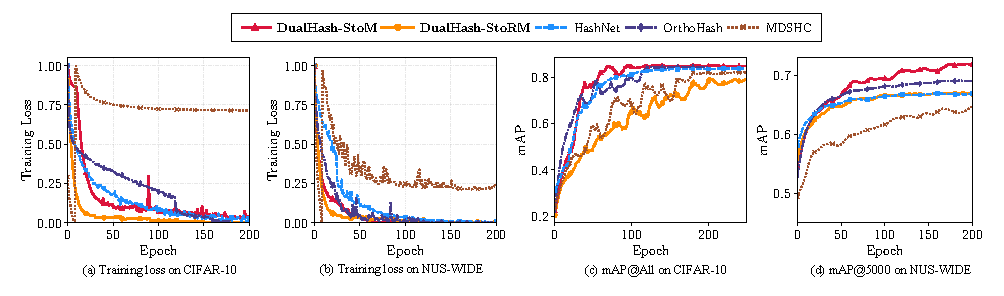
\includegraphics[width=0.95\linewidth]{results_images/ex1_4figures_new.pdf}
    \caption{Training loss and the mAP results of DualHash and baselines for 64-bit codes on CIFAR-10 and NUS-WIDE datasets.}
    \label{fig:training_loss_map_2datasets}
    \vspace{-2ex}
\end{figure}
\begin{figure}[t]
    % \vspace{-1mm}
    \centering
    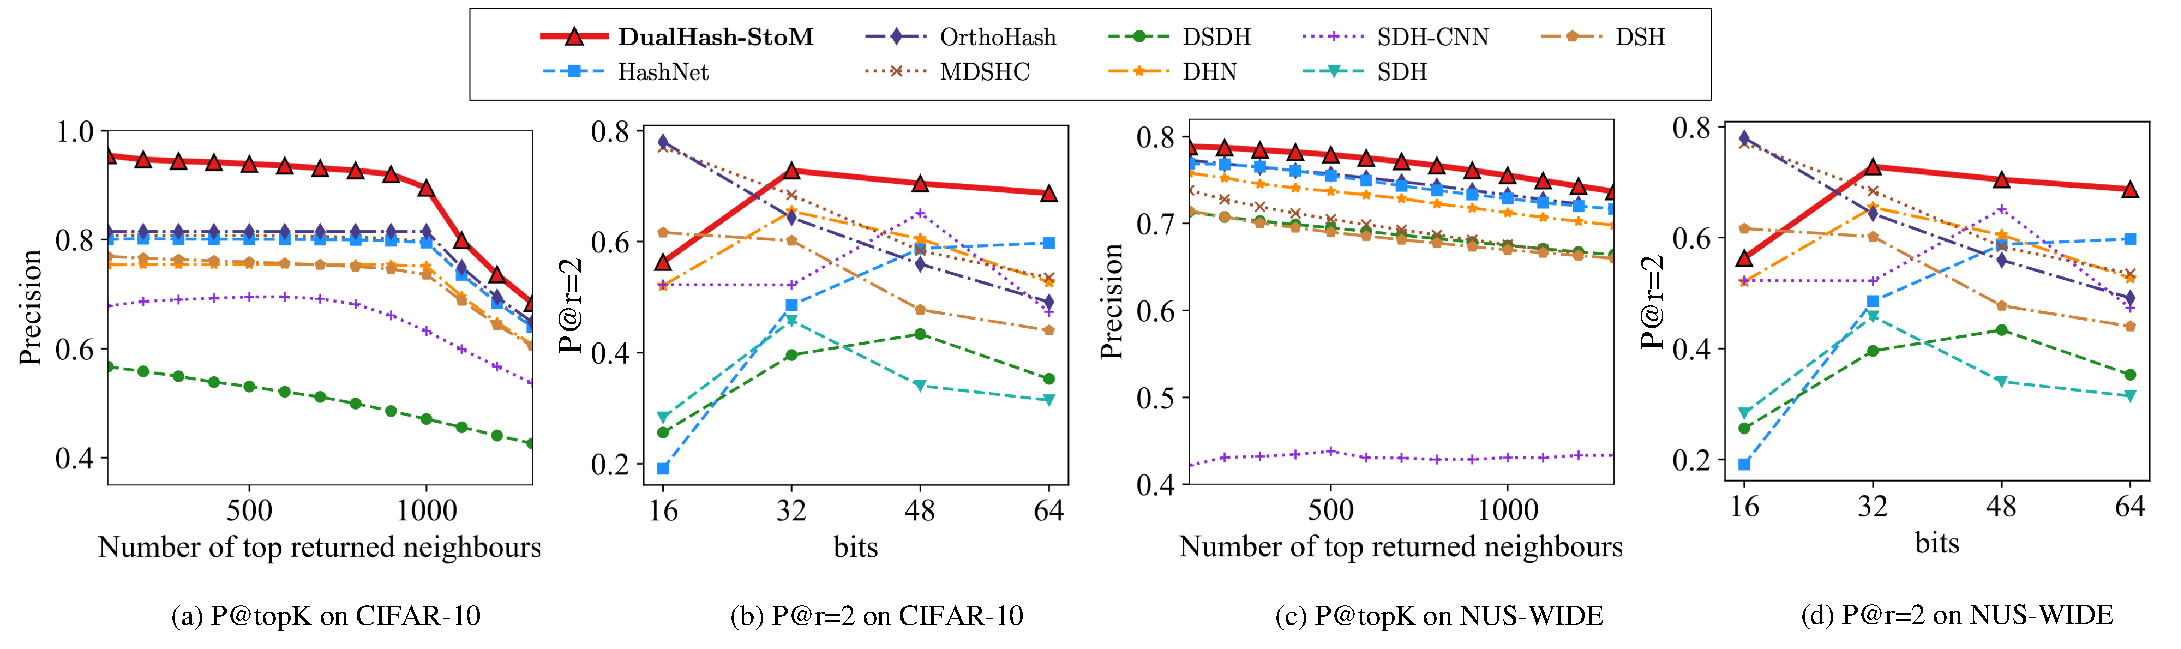
\includegraphics[width=0.95\linewidth]{results_images/ex2_4figures.pdf}
    \caption{Retrieval performance of DualHash and baselines on CIFAR-10 and NUS-WIDE datasets. (a), (c): P@topK for 64-bit codes; (b), (d): P@r=2 with different numbers of bits.}
 \label{fig:retrieval_2datasets}
    \vspace{-2ex}
\end{figure}
\begin{table}[t]
    \centering
    \caption{The mAP results of DualHash and baselines with different numbers of bits on CIFAR-10 and NUS-WIDE datasets with the ResNet-50 backbone.}
    \label{Table: performance_comparison_resnet50_small}
    \resizebox{\linewidth}{!}{
    \begin{tabular}{ccccccccc}
        \toprule
         & \multicolumn{4}{c}{CIFAR-10 (mAP@All)} & \multicolumn{4}{c}{NUS-WIDE (mAP@5000)} \\
        \cmidrule(lr){2-5} \cmidrule(lr){6-9}
         Method (ResNet-50) & 16 bits & 32 bits & 48 bits & 64 bits & 16 bits & 32 bits & 48 bits & 64 bits \\
        \midrule
        DSH \cite{liuDeepSupervisedHashing} & 0.7403 & 0.8116 & 0.8217 & 0.8239 & 0.5559 & 0.6952 & 0.6981 & 0.7165 \\
        OrthoHash \cite{hoeOneLossAll2021} & \textbf{0.9032} & 0.9182 & 0.9202 & 0.9224 & \textbf{0.7448} & 0.7600 & 0.7569 & 0.7863 \\
        MDSHC \cite{wang2023deep} & 0.8980 & 0.9007 & 0.9063 & 0.9227 & 0.6428 & 0.7002 & 0.7248 & 0.7758 \\
        \cmidrule(lr){2-9}
        DualHash-StoM & 0.8559 & \textbf{0.9202} & \textbf{0.9392} & \textbf{0.9416} & 0.6538 & \textbf{0.7783} & \textbf{0.7721} & \textbf{0.8016} \\
        \bottomrule
    \end{tabular}}
    \vspace{2ex}
    \parbox{\linewidth}{\footnotesize
    \textbf{Bold} values indicate the best results.
    }
    \vspace{-1ex}
\end{table}
We provide empirical evidence that is consistent with our theoretical results (Theorems \ref{Theorem: the oracle complexity in SGDM} and \ref{Theorem: the oracle complexity in STORM}) and compare with HashNet, OrthoHash, and MDSHC with 64-bit codes on CIFAR-10 and NUS-WIDE. 
\Cref{fig:training_loss_map_2datasets} shows the training loss and validation mAP curves over epochs.
\red{As shown in \Cref{fig:training_loss_map_2datasets} (a)\blue{--}(b), the StoRM curves reach lower training losses earlier than the StoM curves on CIFAR-10 and NUS-WIDE; the CIFAR-10 curve reaches this level after approximately 25 epochs. The StoM curves reach comparable losses after approximately 75 epochs on CIFAR-10.} \red{\Cref{fig:training_loss_map_2datasets} (c)\blue{--}(d) show that the StoM and StoRM variants have different validation-mAP trajectories, with the StoM variant attaining the higher final value in this comparison.}
% \vspace{3pt}
\subsection{Comparison of Retrieval Performance}
\label{Subsection: Comparison of retrieval performance}
\begin{table}[t]
% \vspace{2ex}
    \centering
    \caption{The mAP results of DualHash and baselines with different numbers of bits on the ImageNet-100 dataset with the ResNet-50 backbone.}
    \label{tab:performance_imagenet_resnet50}
    \small
    \begin{tabular}{lcccc}
     \toprule
 & \multicolumn{4}{c}{ImageNet-100 (mAP@1000)} \\
\cmidrule(lr){2-5}
Method (ResNet-50) & 16 bits & 32 bits & 48 bits & 64 bits \\
\midrule
DSH \cite{liuDeepSupervisedHashing} & 0.7179 & 0.7448 & 0.7335 & 0.7585 \\
OrthoHash \cite{hoeOneLossAll2021} & 0.8040 & \textbf{0.8292} & 0.8510 & 0.8636 \\
MDSHC \cite{wang2023deep} & \textbf{0.8047} & 0.8131 & 0.8561 & 0.8657 \\
 \cmidrule(lr){2-5}
DualHash-StoM & 0.7402 & 0.7705 & \textbf{0.8662} & \textbf{0.8714} \\
        \bottomrule
    \end{tabular}
    \vspace{2ex}
    \parbox{\linewidth}{\footnotesize
    \textbf{Bold} values indicate the best results.
    }
    \vspace{-2ex}
\end{table}
We report retrieval performance on CIFAR-10 and NUS-WIDE datasets, as shown in Tables \ref{Table: baselines mAP}
% , \ref{Table: performance_comparison_resnet50_small}, \ref{tab:performance_imagenet_resnet50} 
and \ref{fig:retrieval_2datasets}. 
\red{The tables report mAP values for DualHash and the listed baselines. On CIFAR-10, DualHash-StoM reports 0.8539 mAP with 64-bit codes, compared with 0.8355 for OrthoHash; on NUS-WIDE, it reports 0.7448, compared with 0.6493 for MDSHC. The StoRM variant has lower mAP than StoM in these settings.}

\red{We also evaluate the methods with a ResNet-50 backbone. In \Cref{Table: performance_comparison_resnet50_small}, DualHash-StoM reports 0.9416 mAP on CIFAR-10 and 0.8016 on NUS-WIDE at 64 bits. In \Cref{tab:performance_imagenet_resnet50}, it reports 0.8662 and 0.8714 mAP on ImageNet-100 at 48 and 64 bits, respectively. The best-performing method varies with the dataset and code length.}

\red{For P@topK (\Cref{fig:retrieval_2datasets} (a),(c)), the curves report precision values for the compared methods, with DualHash reaching approximately 0.9 at low top-$k$ values on CIFAR-10. For P@r=2 (\Cref{fig:retrieval_2datasets} (b),(d)), the reported curves vary with the code length; the 32-bit setting is competitive in the displayed CIFAR-10 and NUS-WIDE comparisons.}
% \vspace{3pt}

\subsection{Quantization Error Analysis}
\label{Subsection: Further analysis}
\begin{figure}[thbp]
% \vspace{-2ex}
    \centering
    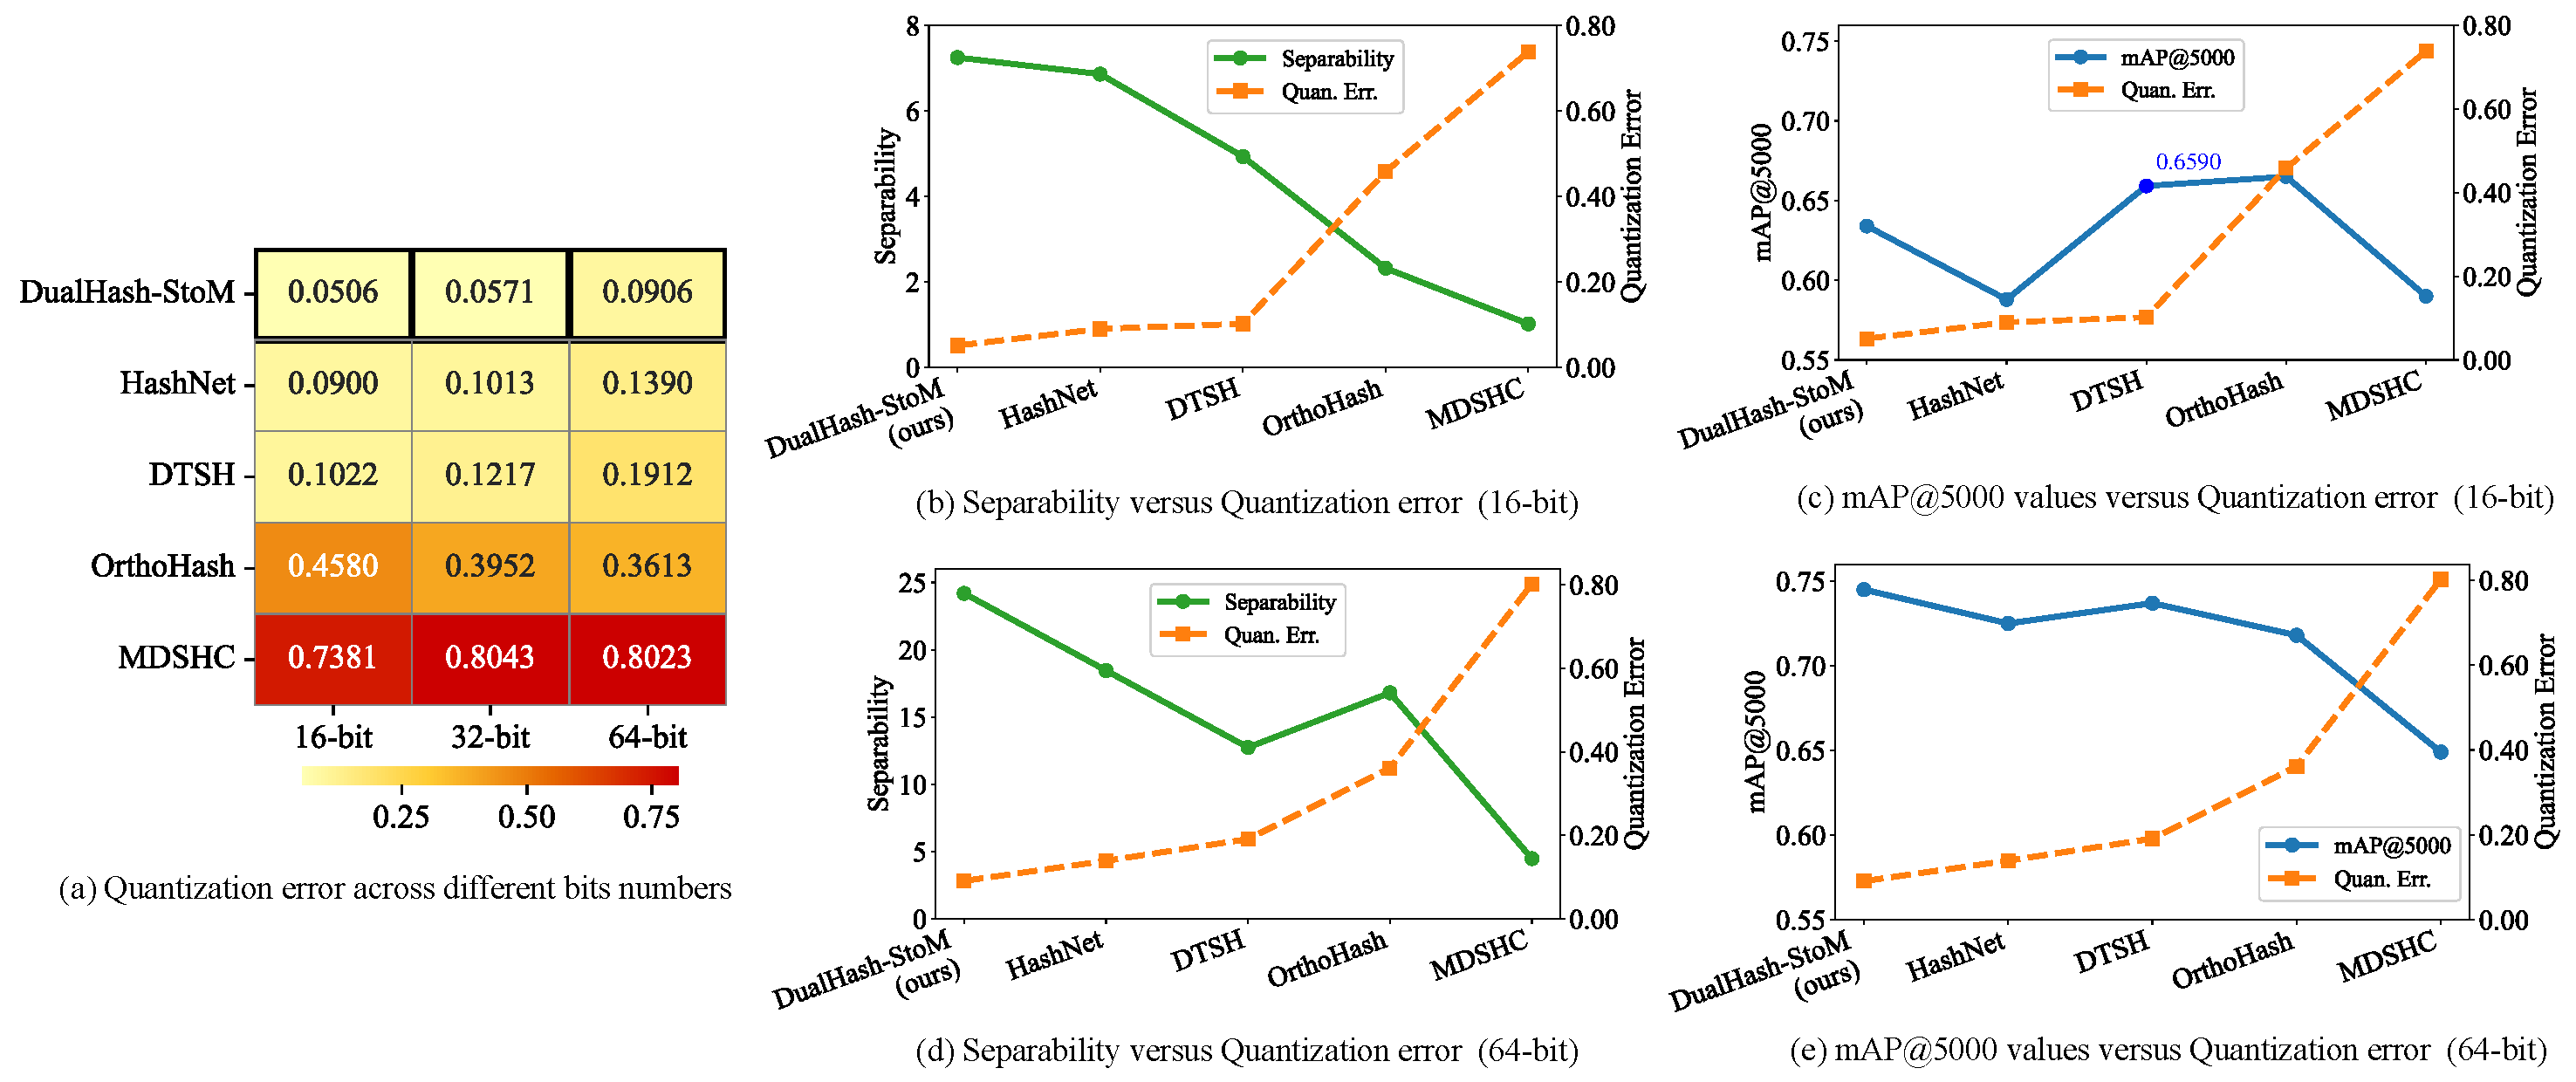
\includegraphics[width=0.95\linewidth]{results_images/quantization_error_further_analysis.pdf}
    \caption{Quantization error and its impact on retrieval performance across different numbers of bits on  NUS-WIDE.}
    \label{fig:quantization_error}
\end{figure}
\begin{figure}[thbp]
    % \vspace{-2ex}
    \centering
    \includegraphics[width=0.95\linewidth]{results_images/hamming_hig_64.pdf}
    \caption{Histogram of intra-class and inter-class Hamming distances of DualHash and baselines for 64-bit codes on the NUS-WIDE dataset. The arrow annotation is the separability in Hamming distances, \(\EE [D_{inter}] - \EE [D_{intra}]\). We normalized the frequency so that the sum over all bins equals 1.}
    \label{fig:His_64_NUSWIDE}
    \vspace{-2ex}
\end{figure}
\begin{figure}[thbp]
    % \vspace{-2ex}
    \centering
    \includegraphics[width=0.95\linewidth]{results_images/hamming_hig_16.pdf}
    \caption{Histogram of intra-class and inter-class Hamming distances of DualHash and baselines with 16-bit codes on NUS-WIDE.}
    \label{fig:His_16_NUSWIDE}
    \vspace{-2ex}
\end{figure}
\begin{figure}[thbp]
    % \vspace{-1mm}
    \centering
    \includegraphics[width=0.95\linewidth]{results_images/sensitivity_2datasets.pdf}
    \caption{The mAP results of DualHash-StoM with different settings of \(\eta\) and \(\lambda\) for 64-bit and 16-bit codes on CIFAR-10 and NUS-WIDE.}
    \label{fig:sensitivity_analysis_DualHash}
    \vspace{-2ex}
\end{figure}
To elucidate the mechanisms behind the performance of DualHash, following \cite{hoeOneLossAll2021},
we examine the quantization error (the discrepancy between continuous outputs and binary codes, \Cref{fig:quantization_error}) and the Hamming distance distributions of the resulting hash codes (\Cref{fig:His_64_NUSWIDE,fig:His_16_NUSWIDE}) across different bit lengths $K$ on the NUS-WIDE dataset. The reported quantization error is the average per-bit error $Q_1/(nd)$ defined by \eqref{eq:quantization-error}, evaluated over the outputs used in this comparison. We compare DualHash-StoM against four deep hashing methods: HashNet \cite{Cao2017HashNetDL} and OrthoHash \cite{hoeOneLossAll2021} (employing distinct quantization strategies), and DTSH \cite{wang2016DTSH} and MDSHC \cite{wang2023deep} (both utilizing \blue{W-type regularization}).

% \vspace{3pt}
\red{\noindent\textbf{(1) Quantization Error and Hamming-Distance Distributions.}
We observe an association between the reported quantization errors and the intra- and inter-class distance distributions in \Cref{fig:quantization_error}(a) and \Cref{fig:His_16_NUSWIDE,fig:His_64_NUSWIDE}. In the 64-bit setting (\Cref{fig:His_64_NUSWIDE}), HashNet and DualHash have similar inter-class distributions near the Hamming distance $K/2=32$. DualHash reports a quantization error of 0.0906 versus 0.1390 for HashNet, while MDSHC reports 0.8023 and a different distance distribution. The corresponding separability ratios in the plotted comparison are 24.19 for DualHash and 4.47 for MDSHC. These observations describe the association between quantization error and the displayed distance statistics; they do not by themselves establish a causal effect.}

% \vspace{3pt}
\red{\noindent\textbf{(2) Quantization Error of DualHash.}
As shown in \Cref{fig:quantization_error}(a), DualHash reports the smallest quantization error among the evaluated methods at the displayed bit lengths. This empirical result is associated with the dual-space reformulation of the \blue{W-type regularization}; the convex conjugate supplies the componentwise proximal update used by the algorithm. The experiment does not isolate the contribution of this reformulation from other implementation choices.}

% \vspace{3pt}
\noindent\textbf{(3) Bit-Dependent Performance and the Separability-Semantics Trade-off.}
\red{The displayed relation between quantization error and separability varies across bit settings (\Cref{fig:quantization_error}(b) and (d)), and the corresponding mAP values do not follow a single monotone pattern.}

\red{\noindent\(\triangleright\) \textit{High-bit regime ($K = 64$): the displayed mAP and quantization-error values.}
At $K=64$ (Figures \ref{fig:quantization_error}(d) and (e)), the methods with lower reported quantization errors also have higher mAP in the displayed comparison. This is an empirical association; the figures do not identify a causal mechanism.}

\red{\noindent\(\triangleright\) \textit{Low-bit regime ($K = 16$): the association is not monotone.}
At $K=16$ (\Cref{fig:quantization_error}(b) and (c)), methods with both low and high reported quantization errors can have lower mAP in the displayed comparisons, while DTSH has an intermediate error and higher mAP in those plots. The relation between quantization error and retrieval performance therefore varies with the dataset and code length.}

% \vspace{3pt}
\subsection{Parameter Sensitivity Analysis}
To explore the sensitivity of key hyperparameters $\eta$ and $\lambda$ in 
DualHash, we conduct a grid search with $\eta \in \{10^{-4}, 10^{-3}, 
10^{-2}, 10^{-1}\}$ and $\lambda \in \{10^{-3}, 10^{-2}, 5\times 10^{-2}, 10^{-1}\}$. Unlike many deep hashing 
methods that exhibit significant hyperparameter sensitivity, the DualHash-StoM
curves show limited variation across a range of hyperparameter
combinations (see \Cref{fig:sensitivity_analysis_DualHash}). 
\red{Specifically, the 64-bit curves show mAP variations below 3\% on CIFAR-10 and 8\% on NUS-WIDE, whereas the 16-bit curves show greater sensitivity, up to 18\% on CIFAR-10. Overall, the displayed sensitivity curves show smaller variation for the 64-bit setting than for the 16-bit setting.}

\section{Conclusion and Discussion}
\label{Section: Conclusion}
+\red{This paper developed DualHash, a stochastic primal--dual method for deep hashing with W-type regularization. The analysis first characterizes the convex envelope $h^{**}$ and its contact set, then gives an exact stationarity correspondence for KKT points of the conjugate formulation and a near-stationarity certificate for the original objective $J_0$. The certificate separates an optimization term controlled by the KKT residual from a structural term controlled by $h(\mathcal{D}(\bx))$; for the $\ell_1$ penalty, the latter is $\lambda Q_1(\bx)$. Under the stated assumptions, DualHash-StoM and DualHash-StoRM attain oracle complexities of $\mathcal{O}(\varepsilon^{-4})$ and $\mathcal{O}(\varepsilon^{-3})$, respectively, for $\varepsilon$-KKT points. The experiments report mAP, precision, and quantization error for CIFAR-10, NUS-WIDE, and ImageNet-100 across code lengths, with the observed rankings varying across datasets and bit lengths.}

\red{The same conjugate construction may also be useful in other composite problems with nonsmooth W-type penalties, but establishing such extensions requires separate analysis.}

% \begin{remark}\label{rmk:penalty-surrogate}
% For any fixed $\gamma > 0$, the penalty problem \eqref{Prop: block-wise regularized problem} 
% is a surrogate of the constrained formulation and is not equivalent to the 
% original problem \eqref{Eq: the primal deep hashing problem}. All convergence 
% results in this paper (Theorems~\ref{Theorem: the oracle complexity in SGDM} 
% and~\ref{Theorem: the oracle complexity in STORM}) are established for the 
% Lagrangian of~\eqref{Prop: block-wise regularized problem}. 
% A formal characterization of the gap between stationary points of 
% \eqref{Prop: block-wise regularized problem} and those of the original 
% composite problem as $\gamma \to \infty$ is an interesting direction 
% for future work.
% \end{remark}


\bibliographystyle{siamplain}
\bibliography{refers}
\newpage
\appendix
\section*{\textbf{Appendix}}
\blue{This appendix contains the proofs of the theoretical results in \Cref{Section: Convergence analysis} and additional experimental material. 

\Cref{Appendix: optimality properties} proves the two propositions in \Cref{Sec: first-order optimality conditions} and defines the stationarity measure $\bd^k$ used in the subsequent analysis. 

\Cref{app-toc-1} collects the bounds and estimates shared by both algorithms. 

\Cref{app-toc-8,app-toc-13} contain the complexity analyses of DualHash-StoM and DualHash-StoRM, respectively. 

\Cref{app-toc-19,app-toc-22} provide the experimental details and additional experimental results.}

\begingroup
\section*{Contents of Appendices}
\leavevmode\par
\hypersetup{hidelinks}
\setlength{\parskip}{0.5em}
\noindent \hyperref[Appendix: optimality properties]{\textbf{Appendix \ref*{Appendix: optimality properties}}\quad Proofs of Propositions in \Cref{Sec: first-order optimality conditions}} \dotfill \pageref{Appendix: optimality properties}\par
\noindent \hspace*{2em} \hyperref[app-toc-zerogap]{\textbf{\ref*{app-toc-zerogap}}\quad Proof of \Cref{prop:zerogap}} \dotfill \pageref{app-toc-zerogap}\par
\noindent \hspace*{2em} \hyperref[Subsec: proof transfer]{\textbf{\ref*{Subsec: proof transfer}}\quad Proof of \Cref{prop:transfer}} \dotfill \pageref{Subsec: proof transfer}\par
\noindent \hyperref[app-toc-1]{\textbf{Appendix \ref*{app-toc-1}}\quad Auxiliary Results for the Complexity Analysis} \dotfill \pageref{app-toc-1}\par
\noindent \hspace*{2em} \hyperref[Subsec: bounds for complexity analysis]{\textbf{\ref*{Subsec: bounds for complexity analysis}}\quad Bounds Used in the Complexity Analysis} \dotfill \pageref{Subsec: bounds for complexity analysis}\par
\noindent \hspace*{2em} \hyperref[Subsec: estimates for common updates]{\textbf{\ref*{Subsec: estimates for common updates}}\quad Estimates for the Common Updates} \dotfill \pageref{Subsec: estimates for common updates}\par
\noindent \hyperref[app-toc-8]{\textbf{Appendix \ref*{app-toc-8}}\quad Complexity Analysis of DualHash-StoM (\Cref{alg:our_algorithm_sgdm})} \dotfill \pageref{app-toc-8}\par
\noindent \hspace*{2em} \hyperref[app-toc-9]{\textbf{\ref*{app-toc-9}}\quad Proof of \Cref{Lemma: One-iteration progress of x in SGDM}} \dotfill \pageref{app-toc-9}\par
\noindent \hspace*{2em} \hyperref[app-toc-10]{\textbf{\ref*{app-toc-10}}\quad Proof of \Cref{Lemma: approximate sufficient descent property in SGDM}} \dotfill \pageref{app-toc-10}\par
\noindent \hspace*{2em} \hyperref[app-toc-11]{\textbf{\ref*{app-toc-11}}\quad Proof of \Cref{lemma: convergence rate sgdm}} \dotfill \pageref{app-toc-11}\par
\noindent \hspace*{2em} \hyperref[app-toc-12]{\textbf{\ref*{app-toc-12}}\quad Proof of \Cref{Theorem: the oracle complexity in SGDM}} \dotfill \pageref{app-toc-12}\par
\noindent \hyperref[app-toc-13]{\textbf{Appendix \ref*{app-toc-13}}\quad Complexity Analysis of DualHash-StoRM (\Cref{alg:our_algorithm_storm})} \dotfill \pageref{app-toc-13}\par
\noindent \hspace*{2em} \hyperref[app-toc-14]{\textbf{\ref*{app-toc-14}}\quad Proof of \Cref{Lemma: One-iteration progress of x in STORM}} \dotfill \pageref{app-toc-14}\par
\noindent \hspace*{2em} \hyperref[app-toc-15]{\textbf{\ref*{app-toc-15}}\quad Proof of \Cref{Lemma: approximate sufficient descent property storm}} \dotfill \pageref{app-toc-15}\par
\noindent \hspace*{2em} \hyperref[app-toc-16]{\textbf{\ref*{app-toc-16}}\quad Proof of the Averaged Stationarity Error Bound for DualHash-StoRM} \dotfill \pageref{app-toc-16}\par
\noindent \hspace*{2em} \hyperref[app-toc-17]{\textbf{\ref*{app-toc-17}}\quad Proof of \Cref{Lemma: convergence rate of storm}} \dotfill \pageref{app-toc-17}\par
\noindent \hspace*{2em} \hyperref[app-toc-18]{\textbf{\ref*{app-toc-18}}\quad Proof of \Cref{Theorem: the oracle complexity in STORM}} \dotfill \pageref{app-toc-18}\par
\noindent \hyperref[app-toc-19]{\textbf{Appendix \ref*{app-toc-19}}\quad Experiment Details} \dotfill \pageref{app-toc-19}\par
\noindent \hspace*{2em} \hyperref[app-toc-20]{\textbf{\ref*{app-toc-20}}\quad Deep Pairwise Supervised Hashing Formulation} \dotfill \pageref{app-toc-20}\par
\noindent \hspace*{2em} \hyperref[app-toc-21]{\textbf{\ref*{app-toc-21}}\quad Implementation Details} \dotfill \pageref{app-toc-21}\par
\noindent \hyperref[app-toc-22]{\textbf{Appendix \ref*{app-toc-22}}\quad Additional Experimental Results} \dotfill \pageref{app-toc-22}\par
\noindent \hspace*{2em} \hyperref[app-toc-23]{\textbf{\ref*{app-toc-23}}\quad Comparison of Optimization Algorithms with Different W-Type Regularizations} \dotfill \pageref{app-toc-23}\par
\noindent\hrulefill
\endgroup
\newpage
\section{\blue{Proofs of the Regularizer and Optimality Properties}}
\label{app:optimality-properties}
\subsection{\blue{Proof of \Cref{lem:wtype-conj}}}
\label{app:wtype-conjugate-proof}
\begingroup\color{blue}
\begin{proof}
Let \(\psi(t):=\phi(\max\{|t|,1\})\). By \ref{W1}--\ref{W2}, \(\phi\) is convex and nonnegative on \([1,+\infty)\), with \(\phi(1)=0\); hence it is nondecreasing there. Thus \(s\mapsto\phi(\max\{s,1\})\) is convex and nondecreasing on \([0,+\infty)\), so \(\psi\) is convex and satisfies \(\psi\le\phi\). Conversely, any convex \(q\le\phi\) satisfies \(q(\pm1)\le0\), hence \(q\le0=\psi\) on \([-1,1]\), while \(q\le\phi=\psi\) on \(|t|\ge1\). Therefore \(\phi^{**}=\psi\), the largest lower semicontinuous convex minorant of \(\phi\)~\cite[Theorem~12.2]{rockafellar1970convex}. For \(|t|<1\), \ref{W1} gives \(\phi(t)>0=\psi(t)\), proving the contact-set formula.

Evaluating the definition of \(\phi^*\) at \(t=\pm1\) gives \(\phi^*(y)\ge|y|\). Since \(\phi(t_0)>0\) for any \(t_0>1\), convexity on \([1,+\infty)\) implies at least linear growth for large \(t\); evenness gives the same for negative \(t\). Hence \(\operatorname{dom}\phi^*\) contains an open interval around zero. The separable formulas follow from~\cite[Theorem~16.4]{rockafellar1970convex}.
\end{proof}
\endgroup

\subsection{Proof of \Cref{prop:zerogap}}
\label{app:zero-gap-proof}
\begin{proof}
    According to \cite[Theorem 2.158]{temporary-citekey-11039},
    $(\bx^{*}, \bB^{*}, \bLmbd^{*})$ are optimal solutions to the
    primal problem \eqref{Prop: block-wise regularized problem} and the dual problem
    \eqref{Prop: the dual problem} \blue{with zero duality gap} if and only if:
    \begin{align}
        \label{Eq: the sufficient and necessary condition}
        \begin{cases}
        (\bx^{*}, \bB^{*}) \in \argmin\limits_{\bx \in \RR^{q}, \bB \in \RR^{n\times d}}\calL(\blue{\bx, \bB}, \bLmbd^{*}), \\
        0 = h(\bB^{*}) + h^{*}(\bLmbd^{*}) - \langle \bLmbd^{*}, \bB^{*}\rangle.
        \end{cases}
    \end{align}
    The first condition in \eqref{Eq: the sufficient and necessary condition} implies
    that $\bm{0}$ belongs to the subdifferential of $\calL$ with respect to
    $(\bx, \bB)$ at $(\bx^{*}, \bB^{*}, \bLmbd^{*})$. Since $\calL$
    is continuously differentiable in $(\bx, \bB)$, we have
    \begin{align}
        \label{Eq: the sufficient and necessary condition for primal}
        \begin{cases}
        \bm{0} = \blue{\nabla_{\bx}F(\bx^{*}, \bB^{*})},\\
        \bm{0} = \blue{\nabla_{\bB}F(\bx^{*}, \bB^{*})} + \bLmbd^{*}.
        \end{cases}
    \end{align}
    For the second condition in \eqref{Eq: the sufficient and necessary condition},
    \blue{since $h^{**}\le h$, the Fenchel--Young inequality for $h^{**}$ yields
    $\langle\bLmbd^*,\bB^*\rangle\le h^{**}(\bB^*)+h^*(\bLmbd^*)\le h(\bB^*)+h^*(\bLmbd^*)=\langle\bLmbd^*,\bB^*\rangle$.
    Thus $h^{**}(\bB^*)+h^*(\bLmbd^*)=\langle\bLmbd^*,\bB^*\rangle$, which, by the subgradient inversion rule~\cite[Theorem~23.5]{rockafellar1970convex}, gives}
    \begin{align}
        \label{Eq: the sufficient and necessary condition for dual}\bB^{*}\in \partial h^{*}(\bLmbd^{*}).
    \end{align}
    Combining \eqref{Eq: the sufficient and necessary condition for primal} and \eqref{Eq: the sufficient and necessary condition for dual}, we obtain \blue{$\bm{0}\in\mathcal{K}(\bx^{*}, \bB^{*}, \bLmbd^{*})$ with $\mathcal{K}$ in \eqref{Eq: KKT mapping}}, completing the proof.
\end{proof}

\subsection{\blue{Proof of \Cref{prop:transfer}}}
\label{app:transfer-proof}
\begingroup\color{blue}
\begin{lemma}\label{lem:no-inner-stationary}
If \(\phi\) satisfies \ref{W1} and \ref{W3}, then \(0\notin\partial\phi(t)\) for every \(t\in(-1,1)\).
\end{lemma}
\begin{proof}
Fix \(t\in[0,1)\) and \(b\in(t,1)\). If \(t'\in[0,b)\) and \(v\in\hat\partial\phi(t')\), then \ref{W3} with \(s=t'\) and \(t'+h\), \(h\downarrow0\), gives \(v\le-c_b\). At \(t'=0\), evenness gives \(\phi(h)\le\phi(0)-c_b|h|\) for \(h<0\), hence also \(v\ge c_b\); thus \(\hat\partial\phi(0)=\emptyset\). By evenness, Fr\'echet subgradients at points of \((-b,0)\) are at least \(c_b\). Passing to limits, \(\partial\phi(t)\subset(-\infty,-c_b]\cup[c_b,\infty)\) for \(|t|<b\).
\end{proof}

\begin{proof}
    Since \(h^{*}\) is proper, lower semicontinuous, and convex, the subgradient inversion rule~\cite[Theorem~23.5]{rockafellar1970convex} gives
    \begin{align}
        \label{Eq: inversion rule of the conjugate}
        \tilde{\bB}\in\partial h^{*}(\tilde{\bLmbd})
        \iff \tilde{\bLmbd}\in\partial h^{**}(\tilde{\bB})
        \iff h^{**}(\tilde{\bB})+h^{*}(\tilde{\bLmbd})=\langle\tilde{\bLmbd},\tilde{\bB}\rangle.
    \end{align}
    The KKT conditions and \(\tilde{\bLmbd}=-\nabla_{\bB}F(\tilde{\bx},\tilde{\bB})\), \(\nabla_{\bx}F(\tilde{\bx},\tilde{\bB})=\bm{0}\), show that (a) holds if and only if \(\tilde{\bLmbd}\in\partial h(\tilde{\bB})\).

    (b)$\iff$(c). By Lemma~\ref{lem:wtype-conj}, the last equality in \eqref{Eq: inversion rule of the conjugate} is equivalent to \(h(\tilde{\bB})=h^{**}(\tilde{\bB})\), which holds if and only if \(|\tilde b_{ij}|\ge1\) for all \(i,j\).

    (b)$\Rightarrow$(a). By the definition of \(h^{*}\), (b) means that \(\tilde{\bB}\) minimizes \(h(\cdot)-\langle\tilde{\bLmbd},\cdot\rangle\) globally. Fermat's rule~\cite[Theorem~10.1]{Rockafellar1998VariationalA} and \cite[Exercise~8.8(c)]{Rockafellar1998VariationalA} give \(\tilde{\bLmbd}\in\partial h(\tilde{\bB})\).

    (a)$\Rightarrow$(c). By separability~\cite[Proposition~10.5]{Rockafellar1998VariationalA}, each entry satisfies \(\tilde\Lambda_{ij}\in\partial\phi(\tilde b_{ij})\cap\partial\phi^{**}(\tilde b_{ij})\). If \(|\tilde b_{ij}|<1\), Lemma~\ref{lem:wtype-conj} gives \(\partial\phi^{**}(\tilde b_{ij})=\{0\}\), so \(0\in\partial\phi(\tilde b_{ij})\), contradicting Lemma~\ref{lem:no-inner-stationary}. Hence \(|\tilde b_{ij}|\ge1\) for all \(i,j\).
\end{proof}
\endgroup

\noindent\blue{Our complexity bounds concern $\mathbb{E}[\mathrm{dist}^{2}(\bm{0},\mathcal K(\bx^{k},\bB^{k},\bLmbd^{k}))]$.} For $\bd^{k}\in\blue{\mathcal K}(\bx^{k},\bB^{k},\bLmbd^{k})$, let us denote $\bd^{k}=(\bd_{\bx}^{k},\bd_{\bB}^{k},\bd_{\bLmbd}^{k})$ and
\begin{align}
    \label{Eq: the components of the subgradient}
    \begin{cases}&\bd_{\bx}^{k}= \nabla_{\bx}F(\bx^{k}, \bB^{k}),\\&\bd_{\bB}^{k}=\nabla_{\bB}F(\bx^{k}, \bB^{k}) + \bLmbd^{k}, \\&\bd_{\bLmbd}^{k}= \bB^{k}- \calG_{\bLmbd}^{k},\end{cases}
\end{align}
where \blue{$\calG_{\bLmbd}^{1}:=\bB^1\in\partial h^*(\bLmbd^1)$ by proximal optimality in \eqref{eq:proximal-initialization} and subgradient inversion, and $\calG_{\bLmbd}^{k}:=2\bB^{k}-\bB^{k-1}+\tau(\bLmbd^{k-1}-\bLmbd^{k})\in\partial h^{*}(\bLmbd^{k})$ for $k\ge2$ by the optimality condition of the $\bLmbd$-update \eqref{Eq: the update of lambda}, implying}
\begin{align}
    \label{Eq: the stationarity error bound in proof}
    \mathrm{dist}^{2}(\bm{0},\blue{\mathcal K}(\bx^{k},\bB^{k},\bLmbd^{k}))\le\|\bd_{\bx}^{k}\|^{2}+\|\bd_{\bB}^{k}\|^{2}+\|\bd_{\bLmbd}^{k}\|^{2}.
\end{align}

\subsection{\blue{Proofs of \Cref{lem:conjugate-minorant,prop:original-certificate}}}
\label{app:original-certificate-proof}
\begingroup
\color{blue}
\paragraph{Conjugate minorant.}
Write $D=\mathcal{D}(\bx)$ and choose $V\in\partial h^*(\bLmbd)$ closest to $\bB$. Such a point exists because this set is nonempty and closed when $r_{\mathcal K}<\infty$. Set
\[
a=\nabla_{\bx}F(\bx,\bB),\qquad b=m(\bB-D)+\bLmbd,\qquad c=\bB-V.
\]
Then $r_{\mathcal K}^2=\|a\|^2+\|b\|^2+\|c\|^2$ and
$\nabla s_{\bLmbd}(\bx)=a+\nabla\mathcal D(\bx)^*b$, which proves~\eqref{eq:minorant-gradient}. The asserted Lipschitz constant follows from Assumption~\ref{Ass: basic regularity}(ii). Fenchel--Young gives $s_{\bLmbd}\le J_0$ and
$J_0(\bx)-s_{\bLmbd}(\bx)\ge h(D)-h^{**}(D)$.
Since $\bLmbd\in\partial h^{**}(V)$, Fenchel equality and $h^{**}\ge0$ yield
\[
\langle\bLmbd,D\rangle-h^*(\bLmbd)
=h^{**}(V)+\frac{\|\bLmbd\|^2}{m}
+\left\langle\bLmbd,c-\frac{b}{m}\right\rangle
\ge-\frac{\|mc-b\|^2}{4m}
\ge-\kappa r_{\mathcal K}^2.
\]
This proves~\eqref{eq:minorant-gap}.

\paragraph{Near-stationarity certificate.}
Let $s\le J_0$ have an $L$-Lipschitz gradient, where $L>0$, and suppose $J_0(\bx)-s(\bx)\le E$. Choose a global minimizer $\widehat{\bx}$ of
\[
H(\by):=J_0(\by)-\langle\nabla s(\bx),\by-\bx\rangle+L\|\by-\bx\|^2.
\]
The lower smoothness bound gives $H(\by)\ge s(\bx)+(L/2)\|\by-\bx\|^2$, so continuity of $J_0$ implies existence of this minimizer. Since $H(\widehat{\bx})\le H(\bx)=J_0(\bx)$,
\[
\|\widehat{\bx}-\bx\|\le\sqrt{2E/L}.
\]
Fermat's rule and the smooth sum rule give
$\nabla s(\bx)-2L(\widehat{\bx}-\bx)\in\partial J_0(\widehat{\bx})$, hence
\[
\operatorname{dist}(\bm0,\partial J_0(\widehat{\bx}))
\le\|\nabla s(\bx)\|+2\sqrt{2LE}.
\]
Applying this argument with $s=s_{\bLmbd}$ and $E=h(\mathcal{D}(\bx))+\kappa r_{\mathcal{K}}^2$, and using \Cref{lem:conjugate-minorant} proves part~(a), including $E=0$. For part~(b), $\bLmbd\in\dom h^*$ implies $\|\bLmbd\|\le\lambda\sqrt{nd}$.

\paragraph{Representative regularizers.}
For $u\in\RR$, $\log\cosh u\le|u|$ and $\operatorname{Hub}_{\delta}(u)\le|u|$. For the squared penalty, Assumption~\ref{Ass: basic regularity}(ii) gives
$\bigl||D_{ij}|-1\bigr|\le\max\{1,C_{\mathcal D}-1\}$.
Multiplying by $\bigl||D_{ij}|-1\bigr|$ and summing proves the bounds in \Cref{rem:certificate-table}.

\paragraph{Multiplier bound and the loss minorant.}
Define $T(U):=m(U-\operatorname{prox}_{h^{**}/m}(U))$. Firm nonexpansiveness of the convex proximal mapping implies that $T$ is $m$-Lipschitz. The residual identities give
$D=V+\bLmbd/m+c-b/m$, so $\bLmbd=T(D-c+b/m)$.
Since $h^{**}$ is separable, vanishes on the cube, and is nondecreasing away from it, each coordinate of $\operatorname{prox}_{h^{**}/m}(D)$ lies between $D_{ij}$ and its projection onto $[-1,1]$. Therefore
\[
\|\bLmbd\|\le\|T(D)\|+\|mc-b\|
\le m\|(|D|-\bm1)_+\|+\sqrt{1+m^2}\,r_{\mathcal K}.
\]
Using $\nabla f(\bx)=\nabla s_{\bLmbd}(\bx)-\nabla\mathcal D(\bx)^*\bLmbd$ and the preceding certificate argument with $s=f$, $L=L_f$, and $E=h(D)$ proves part~(i) of \Cref{rem:certificate-without-conjugate}. At an exact KKT point, $b=c=0$, giving $\bB=\operatorname{prox}_{h^{**}/m}(D)$ and $\bLmbd=T(D)$. For $p=1$, the scalar proximal formula gives $|\Lambda_{ij}|=\min\{m(|D_{ij}|-1)_+,\lambda\}$. On the cube, $T(D)=0$, $\bB=D$, and $\nabla f(\bx)=0$; also $h^*(0)=0$, so $s_{\bm0}=f$. This proves part~(ii).
\endgroup

\section{Auxiliary Results for the Complexity Analysis}
\label{app:complexity-auxiliary-results}

\subsection{\blue{Smoothness Constant of $F$}}
\label{app:smoothness-discussion}
\begingroup\color{blue}
Under Assumption~\ref{Ass: basic regularity}(ii), $F$ is $L_F$-smooth on $\RR^q\times\{\bB:\|\bB\|\le R_B\}$, where
\begin{equation}
\label{eq:derived-smoothness-constant}
L_F:=2L_f+\frac{\gamma}{n}\left(L_{\nabla\mathcal{D}}C_{\mathcal{D}B}+2G_{\mathcal{D}}^2+1\right).
\end{equation}
Here $C_{\mathcal{D}B}:=C_{\mathcal{D}}+R_B$ and
\[
R_B:=C_{\mathcal{D}}+\frac{n\lambda\sqrt{nd}}{\gamma}.
\]
This region contains all primal iterates under the prescribed initializations and step sizes, and $L_F$ is independent of $T$.

\begin{proof}
For a W-type regularizer with compact dual domain, $\bB^1\in\partial h^*(\bLmbd^1)$ and \eqref{Eq: the update of lambda} give $\|\bLmbd^k\|\le\lambda\sqrt{nd}$ for all $k\ge1$.
Since $L_F\ge\gamma/n$, the prescribed step sizes satisfy $0<\tau\gamma/n<1$.
Since $\phi^{**}$ is even and convex, its proximal mapping preserves sign and does not increase magnitude. Thus \eqref{eq:proximal-initialization} and Assumption~\ref{Ass: basic regularity}(ii) give $\|\bB^1\|\le\|\mathcal{D}(\bx^1)\|\le C_{\mathcal{D}}\le R_B$. If $\|\bB^k\|\le R_B$, then \eqref{Eq: the update of B} gives
\[
\|\bB^{k+1}\|\le\left(1-\frac{\tau\gamma}{n}\right)R_B
+\frac{\tau\gamma}{n}C_{\mathcal{D}}+\tau\lambda\sqrt{nd}=R_B,
\]
where the equality follows from the definition of $R_B$. By induction, $\|\bB^k\|\le R_B$ for all $k\ge1$.
Thus $\|\mathcal{D}(\bx)-\bB\|\le C_{\mathcal{D}B}$ throughout the stated region.

For two points $(\bx,\bB)$ and $(\bx',\bB')$ in this region, the gradient of $P(\bx,\bB)=\frac{\gamma}{2n}\|\mathcal{D}(\bx)-\bB\|^2$ satisfies
\begin{align*}
\|\nabla_{\bx}P(\bx,\bB)-\nabla_{\bx}P(\bx',\bB')\|
&\le\frac{\gamma}{n}\left[\left(L_{\nabla\mathcal{D}}C_{\mathcal{D}B}+G_{\mathcal{D}}^2\right)\|\bx-\bx'\|+G_{\mathcal{D}}\|\bB-\bB'\|\right],\\
\|\nabla_{\bB}P(\bx,\bB)-\nabla_{\bB}P(\bx',\bB')\|
&\le\frac{\gamma}{n}\left[G_{\mathcal{D}}\|\bx-\bx'\|+\|\bB-\bB'\|\right],
\end{align*}
by Assumption~\ref{Ass: basic regularity}(ii).
The coefficient matrix of these two bounds is positive semidefinite, so its spectral norm is at most its trace.
Hence $P$ is jointly smooth with constant $\frac{\gamma}{n}(L_{\nabla\mathcal{D}}C_{\mathcal{D}B}+G_{\mathcal{D}}^2+1)$.
Since $F=f+P$, \eqref{eq:derived-smoothness-constant} is a valid smoothness constant.
\end{proof}

\endgroup

\subsection{Proof of \Cref{Lemma: dual boundedness}}
\label{app:dual-difference-proof}
\begin{proof}
    Applying the $\bB$-update~\eqref{Eq: the update of B} at iterations $k+1$ and $k+2$ gives
    \begin{align*}
    \bLmbd^{k+1}-\bLmbd^k
    ={}&\tau^{-1}(\bB^{k+1}-\bB^{k+2})
    +\tau^{-1}(\bB^{k+1}-\bB^k)\\
    &+\nabla_{\bB}F(\bx^{k+1},\bB^k)
    -\nabla_{\bB}F(\bx^{k+2},\bB^{k+1}).
    \end{align*}
    By the $L_F$-smoothness of $F$ under \Cref{Ass: basic regularity}(ii),
    \begin{align*}
    \|\bLmbd^{k+1}-\bLmbd^k\|
    \leq{}&\tau^{-1}\|\bB^{k+2}-\bB^{k+1}\|
    +(\tau^{-1}+L_F)\|\bB^{k+1}-\bB^k\|\\
    &+L_F\|\bx^{k+2}-\bx^{k+1}\|.
    \end{align*}
    Squaring this inequality and using $(a+b+c)^2\leq3(a^2+b^2+c^2)$ proves
    \begin{align}
    \|\bLmbd^{k+1}-\bLmbd^k\|^2
    \leq{}&3\tau^{-2}\|\bB^{k+2}-\bB^{k+1}\|^2
    +3(\tau^{-1}+L_F)^2\|\bB^{k+1}-\bB^k\|^2\notag\\
    &+3L_F^2\|\bx^{k+2}-\bx^{k+1}\|^2,
    \label{Eq: dual boundedness in proof}
    \end{align}
    which is the claimed result.
\end{proof}

\subsection{Proof of \Cref{Lemma: One-iteration progress of B and Lambda}}
\label{app:primal-dual-progress-proof}
\begin{proof}
    \blue{By the descent lemma~\eqref{Eq: the descent lemma} for $F(\bx^{k+1},\cdot)$,
    \[
        F(\bx^{k+1},\bB^{k+1})-F(\bx^{k+1},\bB^{k})\le\langle\nabla_{\bB}F(\bx^{k+1},\bB^{k}),\bB^{k+1}-\bB^{k}\rangle+\frac{L_F}{2}\|\bB^{k+1}-\bB^{k}\|^{2}.
    \]
    The bilinear term satisfies
    \[
        \langle\bB^{k+1},\bLmbd^{k+1}\rangle-\langle\bB^{k},\bLmbd^{k}\rangle=\langle\bLmbd^{k},\bB^{k+1}-\bB^{k}\rangle+\langle\bB^{k+1},\bLmbd^{k+1}-\bLmbd^{k}\rangle,
    \]
    and the $\bB$-update gives
    \[
        \nabla_{\bB}F(\bx^{k+1},\bB^{k})+\bLmbd^{k}=-\tau^{-1}(\bB^{k+1}-\bB^{k}).
    \]
    For the conjugate term, $\calG_{\bLmbd}^{k}\in\partial h^{*}(\bLmbd^{k})$ defined after \eqref{Eq: the components of the subgradient} and the convexity of $h^{*}$ give
    \[
        -h^{*}(\bLmbd^{k+1})+h^{*}(\bLmbd^{k})\le-\langle\calG_{\bLmbd}^{k},\bLmbd^{k+1}-\bLmbd^{k}\rangle.
    \]
    Adding these three relations yields
    \begin{align*}
        &\calL(\bx^{k+1},\bB^{k+1},\bLmbd^{k+1})-\calL(\bx^{k+1},\bB^{k},\bLmbd^{k})\\
        &\le-\Bigl(\tau^{-1}-\frac{L_F}{2}\Bigr)\|\bB^{k+1}-\bB^{k}\|^{2}+\langle\bLmbd^{k+1}-\bLmbd^{k},\bB^{k+1}-\calG_{\bLmbd}^{k}\rangle.
    \end{align*}
    For $k\ge2$, the $\bB$-updates at iterations $k$ and $k-1$ and the expression of $\calG_{\bLmbd}^{k}$ give the identity below. For $k=1$, it follows from $\calG_{\bLmbd}^{1}=\bB^1$, $\bB^0=\bB^1$, and $\nabla_{\bB}F(\bx^1,\bB^1)+\bLmbd^1=\bm{0}$:
    \[
        \bB^{k+1}-\calG_{\bLmbd}^{k}=\tau\bigl(\nabla_{\bB}F(\bx^{k},\bB^{k-1})-\nabla_{\bB}F(\bx^{k+1},\bB^{k})\bigr),
    \]
    and hence}
    \begin{align}
        \label{Eq: the recursive relation of L on B and Lambda} & \calL(\bx^{k+1}, \bB^{k+1}, \bLmbd^{k+1}) - \calL(\bx^{k+1}, \bB^{k}, \bLmbd^{k}) \notag \\
        \leq & - \left(\tau^{-1}- \frac{L_{F}}{2}\right) \|\bB^{k+1}- \bB^{k}\|^{2}+ \Big\langle \bLmbd^{k+1}- \bLmbd^{k}, \tau \Big( \nabla_{\bB}F(\bx^{k}, \bB^{k-1}) - \nabla_{\bB}F(\bx^{k+1}, \bB^{k}) \Big) \Big\rangle.
    \end{align}
    For the inner product term in \eqref{Eq: the recursive relation of L on B and Lambda}, we obtain
    \begin{align}
        \label{Eq: the inner product in the recursive relation of L on B and Lambda} & \langle \bLmbd^{k+1}- \bLmbd^{k}, \tau (\nabla_{\bB}F(\bx^{k}, \bB^{k-1}) - \nabla_{\bB}F(\bx^{k+1}, \bB^{k})) \rangle \notag \\
        \leq & \, \frac{\delta\tau}{2}\|\bLmbd^{k+1}- \bLmbd^{k}\|^{2}+ \frac{\tau}{2\delta}\|\nabla_{\bB}F(\bx^{k+1}, \bB^{k}) - \nabla_{\bB}F(\bx^{k}, \blue{\bB^{k-1}}) \|^{2} \notag \\
        \leq & \, \frac{\delta\tau}{2}\|\bLmbd^{k+1}- \bLmbd^{k}\|^{2}+ \frac{\tau L_{F}^{2}}{2\delta}\left( \|\bx^{k+1}- \bx^{k}\|^{2}+ \|\bB^{k}- \bB^{k-1}\|^{2}\right),
    \end{align}
    where the first inequality follows from the fact that
    $\langle \bu, \bv \rangle \leq \frac{\delta}{2}\|\bu\|^{2}+ \frac{1}{2\delta}\|\bv\|^{2}$ for any $\delta >0$ and the second inequality follows from the $L_F$-smoothness of $F$. Then, \blue{setting $\delta=1/6$ and} substituting \eqref{Eq: the inner product in the recursive relation of L on B and Lambda}
    and \eqref{Eq: dual boundedness in proof} into \eqref{Eq: the recursive relation of L on B and Lambda}
    and rearranging the inequality yields \eqref{item: B and Lambda}.
\end{proof}

Before proceeding, throughout Appendices~\ref{app:stom-complexity} and~\ref{app:storm-complexity}, we adopt the notation, \blue{the probabilistic setting} and intermediate results from \Cref{Section: Convergence analysis}. 

\section{Complexity Analysis of DualHash-StoM (\texorpdfstring{\Cref{alg:our_algorithm_sgdm}}{Algorithm 1})}
\label{app:stom-complexity}

\blue{This appendix proves the complexity results for DualHash-StoM stated in \Cref{Section: complexity of StoM}.}
We first present a lemma on continuously differentiable functions with Lipschitz continuous gradients. Since the analysis also requires the relations among the extrapolated iterates, we next establish the key relationships among the iterates generated by \eqref{Eq: the update of x in SGDM} and \eqref{Eq: extrapolated points in SGDM}.

\begin{proposition}[\blue{Proposition 4.1 in \cite{InertialProximalAlternating}}]
    \label{Pp: relations of xyz} Let $\{\bx^{k}\}_{k \in \mathbb{N}}$,
    $\{\by^{k}\}_{k \in \mathbb{N}}$, and $\{\bz^{k}\}_{k \in \mathbb{N}}$ be sequences
    generated by \eqref{Eq: the update of x in SGDM} and \eqref{Eq: extrapolated points in SGDM}. For all $k \in \mathbb{N}$,
    we have:
    \begin{enumerate}[label=(\roman{*})]
        \item $\|\bx^{k}- \by^{k}\|^{2}= \alpha_{k}^{2}\|\bx^{k}- \bx^{k-1}\|^{2}$,

        \item $\|\bx^{k}- \bz^{k}\|^{2}= \beta_{k}^{2}\|\bx^{k}- \bx^{k-1}\|^{2}$,

        \item $\|\bx^{k+1}- \by^{k}\|^{2}\geq (1 - \alpha_{k})\|\bx^{k+1}- \bx^{k}
            \|^{2}+ \alpha_{k}(\alpha_{k}- 1)\|\bx^{k}- \bx^{k-1}\|^{2}$.
    \end{enumerate}
\end{proposition}

\begin{lemma}
    \label{Lemma: auxiliary lemma for f} Let $f(\bx): \mathbb{R}^{q}\rightarrow \mathbb{R}$
    be a continuously differentiable function with an $L$-Lipschitz continuous gradient.
    Then, for any $\bx,\, \by,\,\blue{\bg} \in \mathbb{R}^{q}$ and any $\bx^{+}\in \mathbb{R}
    ^{q}$ defined by
    \[
        \bx^{+}= \by - \eta \blue{\bg}, \hspace{5pt}\eta > 0,
    \]it holds that
    \begin{align}
        \label{Eq: auxiliary lemma for f}f(\bx^{+}) \leq f(\bx) + \langle \nabla f(\bx) - \blue{\bg}, \bx^{+}- \bx \rangle + \frac{L}{2}\|\bx^{+}- \bx\|^{2}+ \frac{1}{2\eta}\|\bx - \by\|^{2}- \frac{1}{2\eta}\|\bx^{+}- \by\|^{2}.
    \end{align}
\end{lemma}
\begin{proof}
    By the definition of $\bx^{+}$, we obtain that
    \[
        \bx^{+}= \argmin\limits_{\bu \in \mathbb{R}^{q}}\{ \langle \blue{\bg}, \bu
        - \by \rangle + \frac{1}{2\eta}\| \bu - \by\|^{2}\},
    \]
    and hence, in particular, by taking $\bu = \bx$, we obtain
    \begin{align*}
        0 \leq \langle \blue{\bg}, \bx - \bx^{+}\rangle + \frac{1}{2\eta}\| \bx - \by\|^{2}- \frac{1}{2\eta}\| \bx^{+}- \by\|^{2}.
    \end{align*}
    Invoking the descent lemma for a smooth function yields the result. 
\end{proof}

\subsection{Proof of \Cref{Lemma: One-iteration progress of x in SGDM}}
\label{app:stom-primal-progress-proof}

\begin{proof}
    Recalling the equivalent relation:
    \begin{align}
        \label{Eq: the update of x one progress in StoM}\mathcal{L}(\bx^{k+1}, \bm{B}^{k}, \bm{\Lambda}^{k}) - \mathcal{L}(\bx^{k}, \bm{B}^{k}, \bm{\Lambda}^{k}) = F(\bx^{k+1}, \bm{B}^{k}) - F(\bx^{k}, \bm{B}^{k}).
    \end{align}
    Then, applying \eqref{Eq: auxiliary lemma for f} \blue{to $F(\cdot, \bB^{k})$, which is $L_F$-smooth, with $\bx=\bx^{k}$, $\by=\by^{k}$, $\eta=\eta_{k}$, and $\bg=\bg_m^{k}$ (so that $\bx^{+}=\bx^{k+1}$ by \eqref{Eq: the update of x in SGDM}),}
    yields
    \begin{align}
        \label{Eq: the update of theta core}F(\bx^{k+1}, \bm{B}^{k}) \leq & F(\bx^{k}, \bm{B}^{k}) + \langle \nabla_{\bx}F(\bx^{k}, \bm{B}^{k}) - \blue{\bg_m^{k}}, \bx^{k+1}- \bx^{k}\rangle \notag                              \\
        +                                                                 & \frac{L_{F}}{2}\|\bx^{k+1}- \bx^{k}\|^{2}+ \frac{1}{2\eta_{k}}\|\bx^{k}- \bm{y}^{k}\|^{2}- \frac{1}{2\eta_{k}}\|\bx^{k+1}- \bm{y}^{k}\|^{2}.
    \end{align}
    For the inner product term in \eqref{Eq: the update of theta core}, using
    the facts that
    $\langle a, b \rangle \leq \frac{s}{2}\|a\|^{2}+ \frac{1}{2s}\|b\|^{2}$ for
    any $s > 0$ and $\| a - c \|^{2}\leq 2\|a - b \|^{2}+ 2\|b -c\|^{2}$ yields
    { \begin{align}\label{Eq: Inner product for theta}&\langle \nabla_{\bx}F(\bx^{k}, \bm{B}^{k}) - \blue{\bg_m^{k}}, \bx^{k+1}- \bx^{k}\rangle \notag \\ \leq&\,\frac{s}{2}\|\bx^{k+1}- \bx^{k}\|^{2}+ \frac{1}{s}\|\nabla_{\bx}F(\bx^{k}, \bm{B}^{k}) - \nabla_{\bx}F(\bm{z}^{k}, \bm{B}^{k}) \|^{2}+ \frac{1}{s}\|\nabla_{\bx}F(\bm{z}^{k}, \bm{B}^{k}) - \blue{\bg_m^{k}}\|^{2}\notag \\ \leq&\, \frac{s}{2}\|\bx^{k+1}- \bx^{k}\|^{2}+ \frac{L^{2}_{F}}{s}\|\bx^{k}- \bm{z}^{k}\|^{2}+ \frac{1}{s}\|\nabla_{\bx}F(\bm{z}^{k}, \bm{B}^{k}) - \blue{\bg_m^{k}}\|^{2}.\end{align}}
    Setting $s = L_{F}$ in \eqref{Eq: Inner product for theta} and substituting into
    \eqref{Eq: the update of theta core}, then applying \cref{Pp: relations of xyz},
    we obtain
    \begin{align}
        F(\bx^{k+1}, \bm{B}^{k}) & \leq F(\bx^{k}, \bm{B}^{k}) - (\frac{1 - \alpha_{k}}{\eta_{k}}- 2L_{F})\frac{\|\bx^{k+1}- \bx^{k}\|^{2}}{2}\notag                                                                                           \\
                                 & +\,(\frac{\alpha_{k}}{\eta_{k}}+ 2L_{F}\beta_{k}^{2})\frac{\|\bx^{k}- \bx^{k-1}\|^{2}}{2}+ \frac{1}{L_{F}}\|\nabla_{\bx}F(\bm{z}^{k}, \bm{B}^{k}) - \blue{\bg_m^{k}}\|^{2}. \label{Eq: the update of x of L in StoM}
    \end{align}
    Substituting \eqref{Eq: the update of x of L in StoM} into \eqref{Eq: the update of x one progress in StoM}
    yields \eqref{Eq: One-iteration progress of x in SGDM} and completes the proof.
    
    % \begin{align}
    %     \label{item: x}
    %     &\mathcal{L}(\bx^{k+1}, \bm{B}^k, \bm{\Lambda}^k) -\mathcal{L}(\bx^k, \bm{B}^k, \bm{\Lambda}^k)  \notag \\
    %     \leq &\,-(\frac{1 - \alpha_k}{\eta_k}- 2L_F) \frac{ \|\bx^{k+1} - \bx^k \|^2}{2}
    %     + (\frac{\alpha_k}{\eta_k}+ 2L_F\beta_k^2) \frac{\|\bx^k - \bx^{k-1} \|^2}{2} \notag \\
    %     \quad&+ \frac{1}{L_F} \|\nabla_{\bx} F(\bm{z}^k, \bm{B}^k) - \bG^k \|^2.
    % \end{align} 
\end{proof}
\subsection{Proof of \Cref{Lemma: approximate sufficient descent property in SGDM}}
\label{app:stom-descent-proof}
\begin{proof}
    Substituting one-iteration progress \eqref{Eq: One-iteration progress of x in SGDM}
    and \eqref{item: B and Lambda} into \eqref{Eq: One-iteration progress decomposition}
    , we obtain
    \begin{align}
        \label{Eq: One-iteration progress in sgdm} & \calL (\bx^{k+1}, \bB^{k+1}, \bLmbd^{k+1}) - \calL (\bx^{k}, \bB^{k}, \bLmbd^{k}) \notag                                                                                                   \\
        \leq \,                                    & K_{1}\Delta_{\bB}^{k+2}- K_{2}\Delta_{\bB}^{k+1}+ K_{3}\Delta_{\bB}^{k}+ K_{4}\Delta_{\bx}^{k+2}- (K_{5}- K_{3})\Delta_{\bx}^{k+1}+ K_{6}\Delta_{\bx}^{k}+ \frac{1}{L_{F}}\|\be^{k}\|^{2}.
    \end{align}
    Applying the definition of $\Psi_m$ from \eqref{Eq: the Lyapunov function in SGDM}
    to \eqref{Eq: One-iteration progress in sgdm}, rearranging, and taking the
    expectation on both sides, we obtain
    {\small
    \begin{align}
        \label{the descent property of Lyapunov func in SGDM first} & \EE\left[\Psi_m(\mathcal{Q}^{k+1})\right] - \EE\left[\Psi_m(\mathcal{Q}^{k})\right]\notag                                                                               \\
        \leq                                                        & - (C_{1}- K_{1}) \EE[\Delta_{\bm{B}}^{k+2}] -(K_{2}- C_{1}- C_{2}) \EE[\Delta_{\bm{B}}^{k+1}] - (C_{2}- K_{3}) \EE[\Delta_{\bm{B}}^{k}] \notag                     \\
                                                                    & - (C_{3}-K_{4}) \EE[\Delta_{\bx}^{k+2}]- (K_{5}-K_{3}-C_{3}-C_{4}) \EE[\Delta_{\bx}^{k+1}] - (C_{4}- K_{6}) \EE[\Delta_{\bx}^{k}] + \frac{\sigma^{2}}{b_{k}L_{F}}.
    \end{align}}Then, \blue{by \Cref{lem:lyapunov-coef-positivity},} substituting the values of coefficients in \eqref{Eq: the coefficients of the Lyapunov function in SGDM}
    and parameter conditions \eqref{Eq: the parameters conditions of dualhash-sgdm in suppl}
    into \eqref{the descent property of Lyapunov func in SGDM first}, we derive
    \begin{align*}
             & \EE\left[\Psi_m(\mathcal{Q}^{k+1})\right] - \EE\left[\Psi_m(\mathcal{Q}^{k})\right] \nonumber                                                                                                                                                        \\
        \leq & \, -C_{\bB}\left( \EE\left[\Delta_{\bB}^{k+1}\right] + \EE\left[\Delta_{\bB}^{k}\right] \right) -C_{\bx}\left( \EE\left[\Delta_{\bm{x}}^{k+1}\right]+ \EE\left[\Delta_{\bm{x}}^{k}\right] \right) + \frac{\sigma^{2}}{b_{k}L_{F}}.
    \end{align*}which is exactly \eqref{Eq: the descent coefficients of potential function in SGDM},
    thereby completing the proof. 
\end{proof}
The technical proof that the coefficients of $\Psi_m$ in \eqref{Eq: the coefficients of the Lyapunov function in SGDM} and the descent constants $C_{\bB}$, $C_{\bx}$ are indeed positive is given as follows.
\begin{lemma}[Positivity of Lyapunov related coefficients]
    \label{lem:lyapunov-coef-positivity} If parameter conditions \eqref{Eq: the parameters conditions of dualhash-sgdm in suppl}
    hold, then the following inequalities are satisfied:
    \begin{align}
        % \label{Eq: the positive coefficients}
        \begin{cases}K_{5}- K_{3}- C_{3}- C_{4}\geq \nu C_{4}, \\ C_{4}- K_{6}\geq \nu C_{4},\\ C_{4}> 0,\\ C_{\bB}> 0 ,\\ C_{2},\, C_{1}> 0, \\ C_{\bx}> 0.\end{cases} \notag
    \end{align}
\end{lemma}
\begin{proof}
    For $K_{5}- K_{3}- C_{3}- C_{4}$ and $C_{4}- K_{6}$ in \eqref{the descent property of Lyapunov func in SGDM first},
    we obtain by straightforward computations by choosing some $\nu > 0$\blue{, where we recall that $K_{5}= \frac{1 - \alpha_{k}}{\eta_{k}}- 2L_{F}$, $C_{3}= K_{4}$, and $\bar{L}_{F}= 2L_{F}+ K_{3}+ K_{4}$}:
    {\begin{align}
        K_{5}- K_{3}- C_{3}- C_{4}
        &= \frac{1 - \alpha_{k}}{\eta_{k}}- \bar{L}_{F}- (1 + \nu)C_{4}+ \nu C_{4}\notag\\
        &= (1 - \alpha_{k})\left(\frac{1}{\eta_{k}}- \frac{\bar{L}_{F}+ (1 + \nu)C_{4}}{1 - \alpha_{k}}\right) + \nu C_{4}\notag \\
        &\geq \nu C_{4}. \notag % \label{Eq: the scaling of the delta1}
    \end{align}}
    where the last inequality follows from $\alpha_{k}= \alpha$ and
    $\frac{1}{\eta_{k}}= \frac{\bar{L}_{F}+ (1 + \nu)C_{4}}{1 - \alpha}$. Then, \blue{using $\alpha_{k}= \alpha$ and $\beta_{k}= \beta$ from \eqref{Eq: the parameters conditions of dualhash-sgdm in suppl},}
    one has
    \begin{align}
        C_{4}- K_{6} & = C_{4}- \frac{\alpha}{\eta_{k}}- 2L_{F}\beta_{k}^{2}\notag                                                                                                                                   \\
                     & = \frac{1}{1 - \alpha}\left( (1 - \alpha)C_{4}- \alpha\bar{L}_{F}- (1 + \nu)C_{4}\alpha - 2L_{F}\beta^{2}(1 - \alpha) \right)\notag                                                           \\
                     & \blue{=} \frac{1}{1 - \alpha}\left( (1 - 2\alpha - \nu)C_{4}- \alpha \left(\bar{L}_{F}+ \frac{2L_{F}\beta^{2}}{\alpha}\right) \right) + \nu C_{4}+ \frac{2L_{F}\beta^{2}\alpha}{1 - \alpha}\notag \\
                     & \geq \nu C_{4},\notag % \label{Eq: the scaling of the delta2}
    \end{align}where the last inequality follows from $\alpha \in (0, \frac{1 - \nu}{2})$
    and
    $C_{4}= \frac{\bar{L}_{F}+ \frac{2L_F \beta^2}{\alpha}}{1 - 2\alpha - \nu}> 0$.
    We rearrange $\frac{1}{\eta_{k}}$ using the definition of $C_{4}$ and obtain
    $\eta_{k}= \frac{\eta}{L_{F}}$ where $\eta = \frac{(1 - 2\alpha - \nu)/2}{\frac{\bar{L}_{F}}{L_{F}}
    + \frac{(1 + \nu)\beta^{2}}{(1 - \alpha)\alpha}}$.

    Next, we verify that the coefficients of $\Psi_m$ satisfying \eqref{Eq: the coefficients of the Lyapunov function in SGDM}
    and $\tau$ satisfying \eqref{Eq: the parameters conditions of dualhash-sgdm in suppl}
    ensure that $C_{\bB},\, C_{\bx}> 0$. Let $t:=\tau L_F$. \blue{By the definitions of $K_1,K_2,K_3$,}
    \[
        \blue{C_{\bB}=\frac{K_2-K_3-K_1}{2}=\frac{L_F}{2t}\left(1-2t-\frac{13}{2}t^2\right).}
    \]
    \blue{The quadratic $1 - 2t - \frac{13}{2}t^{2}$ is positive if and only if $0 < t < \frac{\sqrt{30}-2}{13}$. Hence selecting
    $\tau \in \left(0, \frac{\sqrt{30}-2}{13L_{F}}\right)$ ensures $C_{\bB}> 0$. Consequently, $C_1=K_1=\frac{1}{2\tau}>0$ and $C_2=\frac{1}{2}(K_2-K_1+K_3)=C_{\bB}+K_3>0$, since $K_3=6\tau L_F^2>0$.}
    \blue{Finally, $C_3=K_4>0$ and $C_{\bx}=\nu C_4>0$. Thus all the stated coefficients are positive under \eqref{Eq: the parameters conditions of dualhash-sgdm in suppl}.}
\end{proof}
\subsection{\blue{Lower Bound of the StoM Potential}}
\label{app:stom-lower-bound}
\begingroup\color{blue}
We first record two estimates that are used here and in \Cref{app:storm-lower-bound}.
Let $t:=\tau L_F$. Both parameter settings \eqref{Eq: the parameters conditions of dualhash-sgdm in suppl} and \eqref{Eq: the parameters conditions in dualhash-storm}--\eqref{Eq: the constants for storm} give $t<\frac{\sqrt{30}-2}{13}<0.27$. Hence, by \eqref{Eq: the coefficients of the Lyapunov function in SGDM},
\[
C_1=K_1=\frac{1}{2\tau},\qquad C_3=K_4=\frac{\tau L_F^2}{2}.
\]
By Appendix~\ref{app:smoothness-discussion}, $\|\bB^k\|\le R_B$ and $\|\bLmbd^k\|\le\lambda\sqrt{nd}$ for all $k\ge1$, and $0\le h^*\le nd\sup_{y\in\operatorname{dom}\phi^*}\phi^*(y)$ on $\operatorname{dom}h^*$ by \Cref{lem:wtype-conj} and the condition on $\phi^*$ in \Cref{Section: W-regularizer}. Therefore $\langle\bB^k,\bLmbd^k\rangle\ge-\lambda\sqrt{nd}\,R_B$ and $\Delta_{\bB}^{k+1}=\frac12\|\bB^{k+1}-\bB^k\|^2\le2R_B^2$, so for both algorithms and every $k\ge1$,
\begin{equation}
\label{eq:lb-common}
\calL(\bx^k,\bB^k,\bLmbd^k)-C_1\Delta_{\bB}^{k+1}
\ge F(\bx^k,\bB^k)-c_1',
\qquad
c_1':=\lambda\sqrt{nd}\,R_B+nd\sup_{y\in\operatorname{dom}\phi^*}\phi^*(y)+\frac{R_B^2}{\tau}.
\end{equation}
It remains to control $C_3\Delta_{\bx}^{k+1}=\frac{\tau L_F^2}{4}\|\bx^{k+1}-\bx^k\|^2$ by $F-\underline{\ell}$. Since $f\ge\underline{\ell}$ by \Cref{Ass: basic regularity}(i) and $P\ge0$, we have $F\ge\underline{\ell}$. Let $\Omega:=\RR^q\times\{\bB:\|\bB\|\le R_B\}$. For $(\bx,\bB)\in\Omega$, the point $(\bx,\bB)-L_F^{-1}\nabla F(\bx,\bB)$ has $\bB$-component $(1-\frac{\gamma}{nL_F})\bB+\frac{\gamma}{nL_F}\mathcal{D}(\bx)$, a convex combination of $\bB$ and $\mathcal{D}(\bx)$ since $L_F\ge\gamma/n$; it therefore lies in the convex set $\Omega$ because $R_B\ge C_{\mathcal{D}}$. The descent lemma on $\Omega$ and $F\ge\underline{\ell}$ give
\begin{equation}
\label{eq:lb-gradient}
\|\nabla F(\bx,\bB)\|^2\le2L_F\bigl(F(\bx,\bB)-\underline{\ell}\bigr),\qquad(\bx,\bB)\in\Omega .
\end{equation}

\begin{lemma}[Lower bound of $\Psi_m$]
\label{Lemma: lower bound of Psi_m}
Under Assumptions~\ref{Ass: basic regularity} and~\ref{Ass: main assumptions} and the parameter conditions \eqref{Eq: the parameters conditions of dualhash-sgdm in suppl}, for every $k\ge1$,
\[
\EE[\Psi_m(\calQ^k)]\ge\Psi_m^*:=\underline{\ell}-c_1,
\qquad
c_1:=c_1'+\frac34\tau\eta^2\sigma^2,
\]
where $c_1'$ is defined in \eqref{eq:lb-common}; $c_1$ is independent of $T$.
\end{lemma}

\begin{proof}
Write $\bm{p}_k:=\bx^k-\bx^{k-1}$. By \eqref{Eq: the update of x in SGDM} and the definition of $\be^k$,
\[
\bx^{k+1}-\bx^k=\alpha\bm{p}_k-\frac{\eta}{L_F}\bigl(\nabla_{\bx}F(\bz^k,\bB^k)+\be^k\bigr).
\]
Since $\|\bB^k\|\le R_B$, the $L_F$-smoothness of $F$ and \eqref{eq:lb-gradient} give
\[
\|\nabla_{\bx}F(\bz^k,\bB^k)\|^2\le2\|\nabla_{\bx}F(\bx^k,\bB^k)\|^2+2L_F^2\beta^2\|\bm{p}_k\|^2
\le4L_F\bigl(F(\bx^k,\bB^k)-\underline{\ell}\bigr)+2L_F^2\beta^2\|\bm{p}_k\|^2 .
\]
Combining these two displays with $\EE\|\be^k\|^2\le\sigma^2$ from \eqref{eq: the gradient error in SGDM} yields
\[
C_3\EE[\Delta_{\bx}^{k+1}]
\le3t\eta^2\,\EE\bigl[F(\bx^k,\bB^k)-\underline{\ell}\bigr]
+\frac{tL_F}{4}\left(3\alpha^2+6\eta^2\beta^2\right)\EE\|\bm{p}_k\|^2
+\frac34\tau\eta^2\sigma^2 .
\]
Under \eqref{Eq: the parameters conditions of dualhash-sgdm in suppl}, $\bar L_F\ge2L_F$ gives $\eta<\frac14$, and $0<1-2\alpha-\nu<1$ gives $C_4\ge\bar L_F\ge2L_F$. With $\alpha<\frac12$ and $\beta<1$,
\[
3t\eta^2<1,
\qquad
\frac{tL_F}{4}\left(3\alpha^2+6\eta^2\beta^2\right)<\frac{9tL_F}{32}<L_F\le\frac{C_4}{2}.
\]
Hence the term $C_4\Delta_{\bx}^k=\frac{C_4}{2}\|\bm{p}_k\|^2$ dominates the $\|\bm{p}_k\|^2$-term. Using \eqref{eq:lb-common} and $C_2\Delta_{\bB}^k\ge0$,
\[
\EE[\Psi_m(\calQ^k)]
\ge\underline{\ell}+\left(1-3t\eta^2\right)\EE\bigl[F(\bx^k,\bB^k)-\underline{\ell}\bigr]-c_1'-\frac34\tau\eta^2\sigma^2
\ge\underline{\ell}-c_1 .
\]
\end{proof}
\endgroup

\subsection{Proof of \Cref{lemma: convergence rate sgdm}}
\label{app:stom-rate-proof}
We then bound the three terms on the right-hand side of \eqref{Eq: the stationarity error bound in proof}.

\begin{lemma}[Stationarity error bound]
    \label{Lemma: Stationarity error bound in SGDM} Under Assumptions~\ref{Ass: basic regularity} and~\ref{Ass: main assumptions},
    for any $k \geq 1$, it holds that
    \begin{align}\label{Eq: the stationarity error bound in SGDM Lemma}
        \EE [\mathrm{dist}^{2}(\bm{0}, \mathcal K(\bx^{k}, \bB^{k}, \bm{\Lambda}^{k}))] \leq S_{1}\EE[ \Delta_{\bB}^{k+1}] + S_{2}\EE[ \Delta_{\bB}^{k}] + S_{3}^{k}\EE[ \Delta_{\bm{x}}^{k+1}] + S_{4}^{k}\EE [\Delta_{\bm{x}}^{k}] + \blue{\frac{3\sigma^{2}}{b_{k}}},
    \end{align}
    where the coefficients are given by
    \begin{align}
        \label{Eq: the coefficients of stationarity error bound in SGDM}\begin{cases}S_{1}&= \blue{4(\tau^{-2}+ 3)},\\ S_{2}&= 4(1 + 3 (1 + \tau L_{F})^{2}),\\ S_{3}^{k}&= 4(3\eta_{k}^{-2}+ L_{F}^{2}+ 3 (\tau L_{F})^{2}),\\ S_{4}^{k}&= 6 ( L^2_{F}\beta_{k}^{2}+ \blue{2} \eta_{k}^{-2}\alpha_{k}^{2}).\end{cases}
    \end{align}
\end{lemma}
% \begin{proof}
% For estimating \(\bd_{\bx}^k\), using the optimality condition of \(\bx^k\), we obtain
% \begin{align}
%     &\|\bd_{\bx}^k\|^2 \notag \\
%     =&\,\|\nabla_{\bx} F(\bx^k, \bm{B}^k) \|^2  \notag\\
%     =&\,\eta_k^{-2} \left\| \eta_k \nabla_{\bx} F(\bx^k, \bm{B}^k) + 0\right\|^2 \notag \\
%     =&\, \eta_k^{-2}  \left\|\eta_k\left( \nabla_{\bx} F(\bx^k, \bm{B}^k) - \bG^k \right) + \bm{y}^k - \bx^{k+1} \right\|^2 \notag \\
%     =&\,\eta_k^{-2} \bigg\|\eta_k\Big(
%     \nabla_{\bx} F(\bx^k, \bm{B}^k) - \nabla_{\bx} F(\bm{z}^k, \bm{B}^k) \notag \\
%     &\qquad + \nabla_{\bx} F(\bm{z}^k, \bm{B}^k)- \bG^k \Big)
%     + \bm{y}^k - \bx^k + \bx^k - \bx^{k+1} \bigg\|^2
%     \label{eq:ineq1} \\
%     \leq&\, 3 \|\nabla_{\bx} F(\bx^k, \bm{B}^k) - \nabla_{\bx} F(\bm{z}^k, \bm{B}^k)\|^2
%     + 3\eta_k^{-2}\|\bx^{k+1} - \bx^k + \bx^k - \bm{y}^k \|^2 \notag \\
%     \quad& + 3 \|\be^k\|^2
%     \label{eq:ineq2} \\
%     \leq&\, 3L_F^2 \|\bx^k - \bm{z}^k \|^2
%     + 6\eta_k^{-2} \left(\|\bx^{k+1} - \bx^k\|^2 + \|\bx^k - \bm{y}^k \|^2\right) \notag \\
%     \quad& + 3 \|\be^k\|^2,
% \end{align} where \eqref{eq:ineq1} is deduced by using the fact that \((a + b+ c)^2 \leq 3(a^2 + b^2 +c^2)\) and \eqref{eq:ineq2} is deduced by the smoothness of \( F(\bx, \bm{B})\) and \((a + b)^2 \leq 2(a^2 + b^2)\).
% Then using \cref{Pp: relations of xyz} concludes
%     \begin{align}
%     \label{Eq: dx}
%     \| \bd_{\bx}^k\| \leq  6( L_F \beta_k^2 + 2 \eta_k^{-2} \alpha_k^2) \Delta_{\bx}^{k} + 12 \eta_k^{-2} \Delta_{\bx}^{k+1} + 3 \| \be^k\|^2
%     \end{align}
%     For estimating  \(\bd^k_{\bB}\), using the optimality condition of \(\bB^k\) and the smoothness of \(F\), we obtain
% \begin{align}
%     \|\bd_{\bB}^k\|^2&= \| \nabla_{\bB} F(\bx^{k+1}, \bB^k)+  \bm{\Lambda}^k + \nabla_{\bB} F(\bx^k, \bB^k) - \nabla_{\bB} F(\bx^{k+1}, \bB^k) \|^2 \notag \\
%                     &= 4 \tau^{-2} \Delta^{k+1}_{\bB}  + 4L_F^2\Delta_{\bx}^{k+1} \label{Eq: dB},
% \end{align} where the last inequality follows from the fact \((a + b)^2 \leq 2(a^2 + b^2)\).

% For estimating \( \|\bd^k_{\bm{\Lambda}}\|^2\),  using the optimality condition of \( \bm{\Lambda}^k \) in \eqref{Eq: the optimality condition of lbda},  we obtain
% \begin{align*}
%         \|\bd^k_{\bm{\Lambda}}\|^2 &\leq 2\tau^{2} \|\bm{\Lambda}^k - \bm{\Lambda}^{k-1} \|^2+ 2\|\bB^{k} - \bB^{k-1}\|^2.
%     \end{align*} Then, substituting \eqref{Eq: dual boundedness} in \cref{Lemma: dual boundedness} into the above inequality yield that
% \begin{align}
% \label{Eq: dLambda}
% \|\bd^k_{\bm{\Lambda}} \|^2 \leq 12 \Delta_{\bB}^{k+1} + 4(1 + 3 (1 + \tau L_F )^2)\Delta_{\bB}^k + 12(\tau L_F)^2\Delta_{\bx}^{k+1} .
% \end{align}
% Then, substituting \eqref{Eq: dx}, \eqref{Eq: dB} and \eqref{Eq: dLambda} into \eqref{Eq: the stationarity error bound in proof} yields \eqref{Eq: the stationarity error bound in SGDM Lemma} and completes the proof. 
% \end{proof}
\begin{proof}
    For estimating $\| \bd_{\bx}^{k}\|^{2}$, using the optimality condition of
    $\bx^{k}$, we obtain
    {\small
    \begin{align}
             & \|\bd_{\bx}^{k}\|^{2}\notag                                                                                                                                                                                                                   \\
        =    & \,\|\nabla_{\bx}F(\bx^{k}, \bm{B}^{k}) \|^{2}\notag                                                                                                                                                                                           \\
        =    & \,\eta_{k}^{-2}\left\| \eta_{k}\nabla_{\bx}F(\bx^{k}, \bm{B}^{k}) + 0\right\|^{2}\notag                                                                                                                                                       \\
        =    & \, \eta_{k}^{-2}\left\|\eta_{k}\left( \nabla_{\bx}F(\bx^{k}, \bm{B}^{k}) - \blue{\bg_m^{k}}\right) + \bm{y}^{k}- \bx^{k+1}\right\|^{2}\notag                                                                                                           \\
        =    & \,\eta_{k}^{-2}\bigg\|\eta_{k}\Big( \nabla_{\bx}F(\bx^{k}, \bm{B}^{k}) - \nabla_{\bx}F(\bm{z}^{k}, \bm{B}^{k}) + \nabla_{\bx}F(\bm{z}^{k}, \bm{B}^{k})- \blue{\bg_m^{k}}\Big) + \bm{y}^{k}- \bx^{k}+ \bx^{k}- \bx^{k+1}\bigg\|^{2}\label{eq:d_x_ineq1} \\
        \leq & \, 3 \|\nabla_{\bx}F(\bx^{k}, \bm{B}^{k}) - \nabla_{\bx}F(\bm{z}^{k}, \bm{B}^{k})\|^{2}+ 3\eta_{k}^{-2}\|\bx^{k+1}- \bx^{k}+ \bx^{k}- \bm{y}^{k}\|^{2}+ 3 \|\be^{k}\|^{2}\label{eq:d_x_ineq2}                                                 \\
        \leq & \, 3L_{F}^{2}\|\bx^{k}- \bm{z}^{k}\|^{2}+ 6\eta_{k}^{-2}\left(\|\bx^{k+1}- \bx^{k}\|^{2}+ \|\bx^{k}- \bm{y}^{k}\|^{2}\right) + 3 \|\be^{k}\|^{2},\label{eq:d_x_ineq3}                                                                      
    \end{align}}where \eqref{eq:d_x_ineq2} is deduced by using the fact that
    $(a + b+ c)^{2}\leq 3(a^{2}+ b^{2}+c^{2})$ and \eqref{eq:d_x_ineq3} is deduced
    \blue{from the $L_F$-smoothness of $F(\cdot, \bB^{k})$} and $(a + b)^{2}\leq 2(a^{2}+ b^{2})$.
    Then applying \Cref{Pp: relations of xyz} to \eqref{eq:d_x_ineq3} concludes
    \begin{align}
        \label{Eq: dx}\| \bd_{\bx}^{k}\|^{2}\leq 6( L^2_{F}\beta_{k}^{2}+ 2 \eta_{k}^{-2}\alpha_{k}^{2}) \Delta_{\bx}^{k}+ 12 \eta_{k}^{-2}\Delta_{\bx}^{k+1}+ 3 \| \be^{k}\|^{2}.
    \end{align}
    For estimating $\|\bd^{k}_{\bB}\|^{2}$, using the $\bB$-update
    \eqref{Eq: the update of B}, \blue{the $L_F$-smoothness of $F$, and the inequality $(a + b)^{2}\leq 2(a^{2}+ b^{2})$}, we obtain
    \begin{align}
        \|\bd_{\bB}^{k}\|^{2} & = \| \nabla_{\bB}F(\bx^{k+1}, \bB^{k})+ \bm{\Lambda}^{k}+ \nabla_{\bB}F(\bx^{k}, \bB^{k}) - \nabla_{\bB}F(\bx^{k+1}, \bB^{k}) \|^{2}\notag \\
                              & \leq4 \tau^{-2}\Delta^{k+1}_{\bB}+ 4L_{F}^{2}\Delta_{\bx}^{k+1}.\label{Eq: dB}
    \end{align}

    \blue{For $k=1$, the initialization gives $\bd_{\bLmbd}^{1}=\bm{0}$, so \eqref{Eq: dLambda} holds. For $k\ge2$, using the $\bm{\Lambda}$-update \eqref{Eq: the update of lambda}, we obtain}
\begin{align}
    \|\bd^{k}_{\bm{\Lambda}}\|^{2} & \leq 2\tau^{2}\|\bm{\Lambda}^{k}- \bm{\Lambda}^{k-1}\|^{2}+ 2\|\bB^{k}- \bB^{k-1}\|^{2}. \notag
\end{align}

    Then, \blue{bounding $\|\bm{\Lambda}^{k}- \bm{\Lambda}^{k-1}\|^{2}$ by \Cref{Lemma: dual boundedness} (with $k$ replaced by $k-1$)}, we obtain
    \begin{align}
        \label{Eq: dLambda}\|\bd^{k}_{\bm{\Lambda}}\|^{2}\leq 12 \Delta_{\bB}^{k+1}+ 4(1 + 3 (1 + \tau L_{F})^{2})\Delta_{\bB}^{k}+ 12(\tau L_{F})^{2}\Delta_{\bx}^{k+1}.
    \end{align}

    Finally, \blue{we substitute} \eqref{Eq: dx}, \eqref{Eq: dB}, and \eqref{Eq: dLambda}
    into \eqref{Eq: the stationarity error bound in proof} \blue{and take} the full expectation
    on both sides, \blue{which leads to} \eqref{Eq: the stationarity error bound in SGDM Lemma},
    completing the proof. 
\end{proof}

% We now establish the convergence rate of \Cref{alg:our_algorithm_sgdm} as follows.
% We set $T$ as the maximum number of iterations and denote 
%     $L_{\Delta}= \frac{\max\{S_{1}, S_{2}, S_{3}, S_{4}\}}{\min\{C_{\bB},
%     C_{\bx}\}}$, $C_{\sigma}= \frac{L_{\Delta}}{L_{F}}+ 3$, and
%     $\Delta_{1}= \Psi_m^{1}- \Psi_m(\mathcal{Q}^{*})$
%     are constants independent of $T$, where \(\Psi_m^{1} = \Psi_m(\calQ^1)\).
% \begin{lemma}[Convergence rate of \Cref{alg:our_algorithm_sgdm}]
%     \label{lemma: convergence rate sgdm} Under the conditions of Lemma \ref{Lemma:
%     approximate sufficient descent property in SGDM}, for any $T \geq 1$, there exists
%     $R$ uniformly selected from $\{2,\ldots,T+1\}$ such that $(\bx^{R}, \bB
%     ^{R}, \bLmbd^{R})$ satisfies \eqref{equ:esp} with
%     \begin{align}
%         \label{Eq: the convergence rate of sgdm}\mathbb{E}[\mathrm{dist}^{2}(0, \partial \mathcal{L}(\bx^{R}, \bB^{R}, \bLmbd^{R}))] \leq \frac{L_{\Delta}\Delta_{1}}{T}+ C_{\sigma}\frac{\sigma^{2}}{b_{k}}.
%     \end{align}
% \end{lemma}
\begin{proof}
    \blue{Under \eqref{Eq: the parameters conditions of dualhash-sgdm in suppl}, $\eta_k=\eta/L_F$, $\alpha_k=\alpha$, and $\beta_k=\beta$ are constant, so $S_3^k=S_3$ and $S_4^k=S_4$. Since the four increment terms are nonnegative, \eqref{Eq: the stationarity error bound in SGDM Lemma} gives}
    {\small
    \begin{align}\label{Eq: the stationarity error bound in SGDM rearrange}
        \mathbb{E}[\mathrm{dist}^{2}(\bm{0}, \mathcal K(\bx^{k}, \bB^{k}, \bLmbd^{k}))] \leq \blue{\max\{S_{1}, S_{2}, S_{3}, S_{4}\}} \EE [\Delta_{\bB}^{k+1}+ \Delta_{\bB}^{k}+ \Delta_{\bx}^{k+1}+ \Delta_{\bx}^{k}] + \blue{\frac{3 \sigma^{2}}{b_{k}}}.\end{align}}
    Similarly, from \eqref{Eq: the descent property of Lyapunov func in SGDM}, we
    obtain
    \[
        \EE [\Psi_m(\mathcal{Q}^{k+1})] - \EE[\Psi_m(\mathcal{Q}^{k})]
        \leq -\min \{ C_{\bB}, C_{\bx}\}\EE[\Delta_{\bB}^{k+1}+ \Delta_{\bB}^{k}+
        \Delta_{\bm{x}}^{k+1}+ \Delta_{\bm{x}}^{k}] + \frac{\sigma^{2}}{b_{k}L_{F}},
    \]
    which yields that
    \[
        \EE[\Delta_{\bB}^{k+1}+ \Delta_{\bB}^{k}+ \Delta_{\bm{x}}^{k+1}+ \Delta_{\bm{x}}
        ^{k}] \leq \frac{1}{\min \{ C_{\bB}, C_{\bx}\}}\left( \EE [\Psi_m(\mathcal{Q}
        ^{k})] - \EE[\Psi_m(\mathcal{Q}^{k+1})] + \frac{\sigma^{2}}{b_{k}L_{F}}
        \right)
    \]
    Substituting this inequality into \eqref{Eq: the stationarity error bound in SGDM rearrange},
    summing over $k = 1, \cdots,T$, and dividing by $T$, we obtain
    \begin{align*}
        &\frac{1}{T}\sumT \mathbb{E}[\mathrm{dist}^{2}(\bm{0}, \mathcal K(\bx
        ^{k}, \bB^{k}, \bLmbd^{k}))]\\
        &\leq \frac{L_{\Delta}}{T}\sumT
        \left(\EE [\Psi_m(\mathcal{Q}^{k})] - \EE [\Psi_m
        (\mathcal{Q}^{k+1})] \right) + \blue{\left( 3 + \frac{L_{\Delta}}{L_F}\right) \frac{\sigma^{2}}{T}\sumT\frac{1}{b_{k}}},
    \end{align*}\blue{Since $\bx^0=\bx^1$ and $\bB^0=\bB^1$, the negative increment terms give $\Psi_m(\calQ^1)\le\calL(\bx^1,\bB^1,\bLmbd^1)$, so $\EE[\Psi_m(\calQ^1)]-\Psi_m^*\le\Delta_1$.} Denoting
    $a_{k}= \mathbb{E}[\mathrm{dist}^{2}(\bm{0}, \mathcal K(\bx^{k}, \bB
    ^{k}, \bLmbd^{k}))]$, we have
    \[
        \frac{1}{T}\sumT a_{k}\leq \frac{L_{\Delta}\Delta_{1}}{T}+ \blue{\left( 3 + \frac{L_{\Delta}}{L_F}
        \right) \frac{\sigma^{2}}{T}\sumT\frac{1}{b_{k}}}.
    \]
    \blue{By selecting $R$ uniformly from $\{1, \ldots, T\}$, independently of the iterates, and applying the law of total expectation,}
    we obtain
    \[
        \mathbb{E}[\mathrm{dist}^{2}(\bm{0}, \mathcal K(\bx^{R}, \bB^{R}
        , \bLmbd^{R}))] \blue{= \frac{1}{T}\sumT a_{k}} \leq \frac{L_{\Delta}\Delta_{1}}{T}+ \blue{\left( 3 + \frac{L_{\Delta}}{L_F}
        \right) \frac{\sigma^{2}}{T}\sumT\frac{1}{b_{k}}},
    \] and complete the proof.
\end{proof}
% From \eqref{Eq: the convergence rate of sgdm}, to achieve $\calO(T^{-1})$
% convergence rate, we need to set $b_{k}= \Theta (T)$. Next, we set
% $b_{k}= b = c_{b}T$ for all $k \geq 1$ in this way and establish the complexity
% results of \Cref{alg:our_algorithm_sgdm} with the parameter conditions \eqref{Eq: the parameters conditions of dualhash-sgdm in suppl}.
\subsection{Proof of \Cref{Theorem: the oracle complexity in SGDM}}
\label{app:stom-oracle-proof}
% \setcounter{proof}{0}
\begin{proof}
    When $b_{k}= b = c_{b}T$, \blue{we have $\frac{1}{T}\sumT\frac{1}{b_{k}}=\frac{1}{c_{b}T}$, and hence \Cref{lemma: convergence rate sgdm} gives}
    \[
        \mathbb{E}[\mathrm{dist}^{2}(\bm{0}, \mathcal K(\bx^{R}, \bB^{R}
        , \bLmbd^{R}))] \leq \frac{1}{T}\left( L_{\Delta}\Delta_{1}+ C_{\sigma}
        \frac{\sigma^{2}}{c_{b}}\right).
    \]
    With the conditions on $T$ in \eqref{Eq: the iterate number upper bound of algorithm SGDM},
    this gives
    $\mathbb{E}[\mathrm{dist}^{2}(\bm{0}, \mathcal K(\bx^{R}, \bB^{R}
    , \bLmbd^{R}))] \leq \varepsilon^{2}$. Then, the oracle complexity
    of SFO is
    \[
        \text{Complexity}= (T-1)b_{k}=\calO(T^{2}) = \calO(\varepsilon^{-4}).
    \]
\end{proof}
\section{Complexity Analysis of DualHash-StoRM (\texorpdfstring{\Cref{alg:our_algorithm_storm}}{Algorithm 2})}
\label{app:storm-complexity}
We adopt the same notation as in \Cref{app:stom-complexity}. 
\subsection{\blue{Proof of \Cref{Lemma: One-iteration progress of x in STORM}}}
\label{app:storm-primal-progress-proof}
\begin{proof}
    \blue{By the $L_F$-smoothness of $F(\cdot,\bB^k)$, the update \eqref{Eq: the update of x in STORM}, and Young's inequality,}
    \blue{\begin{align}
        &\calL(\bx^{k+1},\bB^k,\bLmbd^k)-\calL(\bx^k,\bB^k,\bLmbd^k)\notag\\
        &=F(\bx^{k+1},\bB^k)-F(\bx^k,\bB^k)\notag\\
        &\leq\eta_k\langle\be^k,\bg_s^k\rangle-\eta_k\Bigl(1-\frac{\eta_kL_F}{2}\Bigr)\|\bg_s^k\|^2\notag\\
        &\leq\frac{\eta_k}{2}\|\be^k\|^2-\frac{\eta_k}{2}(1-\eta_kL_F)\|\bg_s^k\|^2\notag\\
        &=\frac{\eta_k}{2}\|\be^k\|^2-(\eta_k^{-1}-L_F)\Delta_{\bx}^{k+1},\notag
    \end{align}}
    \blue{where we used $\nabla_{\bx}F(\bx^k,\bB^k)=\bg_s^k-\be^k$ and $2\Delta_{\bx}^{k+1}=\eta_k^2\|\bg_s^k\|^2$.}
\end{proof}

\subsection{Proof of \Cref{Lemma: approximate sufficient descent property storm}}
\label{app:storm-descent-proof}
\begin{proof}
    Substituting the one-iteration progress \eqref{Eq: the recursive relation of L on x}
    and \eqref{item: B and Lambda} into \eqref{Eq: One-iteration progress decomposition}, we obtain
    \begin{align}
             & \calL (\bx^{k+1}, \bB^{k+1}, \bLmbd^{k+1}) - \calL (\bx^{k}, \bB^{k}, \bLmbd^{k}) \nonumber                                                                                                                                          \\
        \leq & \,\frac{\eta_{k}}{2}\| \be^{k}\|^{2}- (\eta_{k}^{-1}- L_{F}- K_{3}) \Delta_{\bx}^{k+1}+ K_{1}\Delta_{\bB}^{k+2}+ K_{4}\Delta_{\bx}^{k+2}- K_{2}\Delta_{\bB}^{k+1}+ K_{3}\Delta_{\bB}^{k}.\label{Eq: One-iteration progress in storm}
    \end{align}
    Applying the definition of $\Psi_r$ from \eqref{Eq: the Lyapunov function in STORM} into \eqref{Eq: One-iteration progress in storm}, we rearrange the above inequality
    \begin{align}
        \label{the descent property of Lyapunov func in STORM first} & \Psi_r(\mathcal{Q}^{k+1}) - \Psi_r(\mathcal{Q}^{k}) \notag                                                                                         \\
        \leq                                                         & - (C_{1}- K_{1}) \Delta_{\bm{B}}^{k+2}-(K_{2}- C_{1}- C_{2}) \Delta_{\bm{B}}^{k+1}- (C_{2}- K_{3}) \Delta_{\bm{B}}^{k}- (C_{3}-K_{4}) \Delta_{\bx}^{k+2}\notag \\
                                                                     & \blue{-(\eta_{k}^{-1}- L_{F}- K_{3}- C_{3}) \Delta_{\bx}^{k+1}+ \frac{\eta_{k}}{2}\| \be^{k}\|^{2}}.
    \end{align}
    By substituting the Lyapunov function coefficients \eqref{Eq: the coefficients of the Lyapunov function in SGDM} into \eqref{the descent property of Lyapunov func in STORM first} \blue{and taking full expectation}, we obtain \eqref{Eq: the descent property of Lyapunov func in storm}. With $\tau$ satisfying \blue{$0<\tau<\frac{\sqrt{30}-2}{13L_F}$}, \Cref{lem:lyapunov-coef-positivity} guarantees that $C_{\bB}>0$.
\end{proof}

% \subsection{Proof of \Cref{Lemma: Weighted error accumulation}}
% \label{Subsubsec: proof Weighted error accumulation}
\subsection{\blue{Lower Bound of the StoRM Potential}}
\label{app:storm-lower-bound}
\begingroup\color{blue}
\begin{lemma}[Lower bound of the StoRM potential]
\label{Lemma: lower bound of W}
Under Assumptions~\ref{Ass: basic regularity} and~\ref{Ass: main assumptions} and the parameter conditions \eqref{Eq: the parameters conditions in dualhash-storm}--\eqref{Eq: the constants for storm}, for every $k\ge1$,
\[
W_k:=\EE[\Psi_r(\calQ^k)]+\frac{\eta_T}{\rho_T}\EE\|\be^k\|^2\ge\Psi_r^*:=\underline{\ell}-c_1',
\]
where $c_1'$ is defined in \eqref{eq:lb-common} and is independent of $T$.
\end{lemma}

\begin{proof}
By \eqref{Eq: the update of x in STORM} and \eqref{eq:lb-gradient},
\[
C_3\Delta_{\bx}^{k+1}
=\frac{\tau L_F^2\eta_T^2}{4}\|\nabla_{\bx}F(\bx^k,\bB^k)+\be^k\|^2
\le\tau L_F^3\eta_T^2\bigl(F(\bx^k,\bB^k)-\underline{\ell}\bigr)+\frac{\tau L_F^2\eta_T^2}{2}\|\be^k\|^2 .
\]
Since $\tilde L_F\ge L_F$, $\eta_T\tilde L_F\le\frac12$ and $\rho_T\le\frac12$ give $\eta_T\le\frac{1}{2L_F}$ and $\eta_T\rho_T\le\frac{1}{4L_F}$. Therefore
\[
\tau L_F^3\eta_T^2\le\frac t4<1,
\qquad
\frac{\tau L_F^2\eta_T^2}{2}=\frac{\tau L_F^2\eta_T\rho_T}{2}\cdot\frac{\eta_T}{\rho_T}\le\frac t8\cdot\frac{\eta_T}{\rho_T}<\frac{\eta_T}{\rho_T}.
\]
Using \eqref{eq:lb-common} and $C_2\Delta_{\bB}^k\ge0$, we obtain
\[
W_k\ge\underline{\ell}+\left(1-\frac t4\right)\EE\bigl[F(\bx^k,\bB^k)-\underline{\ell}\bigr]+\left(1-\frac t8\right)\frac{\eta_T}{\rho_T}\EE\|\be^k\|^2-c_1'\ge\underline{\ell}-c_1' .
\]
\end{proof}
\endgroup

\subsection{\blue{Auxiliary Results for DualHash-StoRM}}
\label{app:storm-stationarity-proof}
We provide a recursive bound on the gradient error vector $\{\be^{k}\}$ with analysis comparable to those in \cite[Lemma~2\blue{.2}]{xu2023momentum} and \cite[Lemma 8]{shi2025momentum}. \blue{We provide the proof for completeness.}
\begin{lemma}[Recursive bound on gradient error]
    \label{Lemma: Recursive bound on gradient error} Under \Cref{Ass: main assumptions}\blue{(ii) and \Cref{Ass: the mean squared smoothness of F}},
    for any $k \geq 1$, it holds that
    \begin{align}
        \blue{\EE}[\| \be^{k+1}\|^{2}] \leq \left(1 - \rho_{k}\right)^{2}\blue{\EE}[\| \be^{k}\|^{2}] + \frac{2 \rho_{k}^{2}\sigma^{2}}{\blue{b_{k+1}}}+ \frac{4(1 - \rho_{k})^{2}L_{F}^{2}}{\blue{b_{k+1}}}\blue{\EE}\left[\Delta_{\bx}^{k+1}\blue{{}+\Delta_{\bB}^{k+1}}\right]. \notag
    \end{align}
\end{lemma}
\begin{proof}
    \blue{By \eqref{Eq: the stochastic approximate in STORM}, the definition of $\be^{k}$, and $\EE_{k+1}[\tilde{\nabla}_{\bx}F(\bx^{j},\bB^{j};\calJ_{k+1})]=\nabla_{\bx}F(\bx^{j},\bB^{j})$ for $j\in\{k,k+1\}$, we obtain
    \begin{align}
        \EE_{k+1}[\|\be^{k+1}\|^{2}]
        \leq & \,(1-\rho_k)^{2}\|\be^{k}\|^{2}+\frac{2\rho_k^{2}\sigma^{2}}{b_{k+1}}\notag\\
        & \,+\frac{2(1-\rho_k)^{2}}{b_{k+1}}\cdot\frac1n\sum_{i=1}^{n}\|\nabla_{\bx}F_i(\bx^{k+1},\bb_i^{k+1})-\nabla_{\bx}F_i(\bx^{k},\bb_i^{k})\|^{2}\notag\\
        \leq & \,(1-\rho_k)^{2}\|\be^{k}\|^{2}+\frac{2\rho_k^{2}\sigma^{2}}{b_{k+1}}+\frac{4(1-\rho_k)^{2}L_F^{2}}{b_{k+1}}\left(\Delta_{\bx}^{k+1}+\Delta_{\bB}^{k+1}\right)\quad\text{a.s.},\notag
    \end{align}
    where the first inequality follows from $\|\bm a+\bm b\|^{2}\leq2\|\bm a\|^{2}+2\|\bm b\|^{2}$, \Cref{Ass: main assumptions}(ii), and the mini-batch variance bound under uniform sampling without replacement, and the last inequality follows from \Cref{Ass: the mean squared smoothness of F}. Taking the full expectation completes the proof.}
\end{proof}

We now establish a weighted error accumulation bound for the variance-reduced gradient estimator in \Cref{alg:our_algorithm_storm}.
\begin{lemma}[Weighted error accumulation bound]
    \label{Lemma: Weighted error accumulation} Under Assumption\blue{s}~\ref{Ass: basic regularity}, \ref{Ass: main assumptions}, \blue{and~\ref{Ass: the mean squared smoothness of F}} and parameter conditions \blue{\eqref{Eq: the parameters conditions in dualhash-storm}--\eqref{Eq: the constants for storm}}, for any $T \geq 1$, the following weighted cumulative error bound holds:
    \begin{align}
        \blue{\frac{1}{T}\sumT\EE\Bigl[C_{\bB}\bigl(\Delta_{\bB}^{k+1}+\Delta_{\bB}^{k}\bigr)+\frac{1}{4\eta_T}\Delta_{\bx}^{k+1}+\frac{\eta_T}{2}\|\be^{k}\|^{2}\Bigr]\leq\frac{1}{T}\Bigl(\tilde{\Delta}_{1}+\frac{\eta_T\sigma^{2}}{\rho_Tb_1}\Bigr)+\frac{2\eta_T\rho_T\sigma^{2}}{b},}
        \label{Eq: weighted error accumulation bound}
    \end{align}
    where $\tilde{\Delta}_{1}=\blue{\calL(\bx^{1},\bB^{1},\bLmbd^{1})}-\Psi_r^{*}$.
\end{lemma}
\begin{proof}
    Under \blue{\eqref{Eq: the parameters conditions in dualhash-storm}--\eqref{Eq: the constants for storm}, $\eta_T\tilde L_F\le\frac12$, so} we have a lower bound for $C_{\bx}^{k}$ with $C_{\bx}^{k}\geq\frac{1}{2\blue{\eta_T}}>0$. Substituting this inequality into \eqref{Eq: the descent property of Lyapunov func in storm} yields
    \begin{align}
        \EE[\Psi_r(\calQ^{k+1})]-\EE[\Psi_r(\calQ^{k})]\leq\blue{-C_{\bB}\EE[\Delta_{\bB}^{k+1}+\Delta_{\bB}^{k}]}-\frac{1}{2\blue{\eta_T}}\EE[\Delta_{\bx}^{k+1}]+\frac{\blue{\eta_T}}{2}\EE[\|\be^{k}\|^{2}].
        \label{Eq: descent of Psi_r in weighted error bound}
    \end{align}
    \blue{To handle the term $\Delta_{\bB}^{k+1}$ in \Cref{Lemma: Recursive bound on gradient error}, let $r=\tau\gamma/n$ and
    \[
        H_k=(1-r)\|\tau(\bLmbd^{k}-\bLmbd^{k-1})-(\bB^{k}-\bB^{k-1})\|^{2}+r\tau^{2}\|\bLmbd^{k}-\bLmbd^{k-1}\|^{2}
    \]
    with $\bLmbd^{0}=\bLmbd^{1}$. Since the initialization sets $\bB^{0}=\bB^{1}$ and $\bLmbd^{0}=\bLmbd^{1}$, we have $H_1=0$ and $H_k\geq0$. By the $\bB$- and $\bLmbd$-updates, we obtain}
    \begin{align}
        \blue{\Delta_{\bB}^{k+1}\leq\frac{12}{r}\bigl(H_k-H_{k+1}\bigr)+G\,\Delta_{\bx}^{k+1},}
        \label{Eq: tracking of B increments}
    \end{align}
    \blue{where the inequality follows from $r\le\tau L_F<\frac{\sqrt{30}-2}{13}<\frac27$ and the entrywise monotonicity and $1$-Lipschitz continuity of $\operatorname{prox}_{\tau^{-1}h^{*}}$, which give $H_{k+1}-H_k\leq-\frac{r}{8}\bigl(\|\bB^{k}-\bB^{k-1}\|^{2}+\|\tau(\bLmbd^{k}-\bLmbd^{k-1})-(\bB^{k}-\bB^{k-1})\|^{2}\bigr)+146rG_{\mathcal{D}}^{2}\Delta_{\bx}^{k+1}$.}
    From \Cref{Lemma: Recursive bound on gradient error} \blue{and \eqref{Eq: tracking of B increments}}, we obtain
    \begin{align}
        &\blue{\EE[\|\be^{k+1}\|^{2}]+\frac{48L_F^{2}}{br}\EE[H_{k+1}]}\notag\\
        &\blue{\leq(1-\rho_T)\EE[\|\be^{k}\|^{2}]+\frac{48L_F^{2}}{br}\EE[H_{k}]+\frac{2\rho_T^{2}\sigma^{2}}{b}+\frac{4L_F^{2}(1+G)}{b}\EE[\Delta_{\bx}^{k+1}],}
        \label{Eq: error recursion with tracking}
    \end{align}
    where the inequality follows from \blue{$(1-\rho_T)^{2}\leq1-\rho_T$}. \blue{Multiplying \eqref{Eq: error recursion with tracking} by $\frac{\eta_T}{\rho_T}$, adding it to \eqref{Eq: descent of Psi_r in weighted error bound}, and applying $\frac{\eta_T}{\rho_T}\cdot\frac{4L_F^{2}(1+G)}{b}\leq\frac{1}{4\eta_T}$, which is equivalent to the lower bound on $\rho$ in \eqref{Eq: the constants for storm},} yields the following expected descent property of the Lyapunov function $\Psi_r$:
    \begin{align}
        &\blue{\EE\Bigl[\Psi_r(\calQ^{k+1})+\frac{\eta_T}{\rho_T}\Bigl(\|\be^{k+1}\|^{2}+\frac{48L_F^{2}}{br}H_{k+1}\Bigr)\Bigr]-\EE\Bigl[\Psi_r(\calQ^{k})+\frac{\eta_T}{\rho_T}\Bigl(\|\be^{k}\|^{2}+\frac{48L_F^{2}}{br}H_{k}\Bigr)\Bigr]}\notag\\
        &\blue{\leq-\EE\Bigl[C_{\bB}\bigl(\Delta_{\bB}^{k+1}+\Delta_{\bB}^{k}\bigr)+\frac{1}{4\eta_T}\Delta_{\bx}^{k+1}+\frac{\eta_T}{2}\|\be^{k}\|^{2}\Bigr]+\frac{2\eta_T\rho_T\sigma^{2}}{b}.}
        \label{Eq: expected descent of Psi_r with error}
    \end{align}
    Finally, summing up \eqref{Eq: expected descent of Psi_r with error} from $k=1$ to $T$ and dividing by $T$, \blue{together with $H_1=\Delta_{\bB}^{1}=0$, $\EE[\|\be^{1}\|^{2}]\leq\sigma^{2}/b_1$, $H_{T+1}\geq0$, and \Cref{Lemma: lower bound of W},} yields \eqref{Eq: weighted error accumulation bound} and completes the proof.
\end{proof}

We derive an upper stationarity error bound for the iterates generated by \Cref{alg:our_algorithm_storm}.
\begin{lemma}[Stationarity error bound]
    \label{Lemma: Stationarity error bound} Under \Cref{Ass: basic regularity}(ii),
    for any $k \geq 1$, it holds that
    \begin{align}
        \mathrm{dist}^{2}(\bm{0}, \mathcal K(\bx^{k}, \bB^{k}, \bm{\Lambda}^{k})) \leq S_{1}\Delta_{\bB}^{k+1}+ S_{2}\Delta_{\bB}^{k}+ S_{3}^{k}\Delta_{\bm{x}}^{k+1}+ 2 \| \be^{k}\|^{2}, \label{Eq: the stationarity error bound in Lemma in storm}
    \end{align}
    where the coefficients are defined as \eqref{Eq: the coefficients of stationarity error bound in SGDM}.
    % \begin{align}
    % \label{Eq: the  coefficients of stationarity error bound in storm}
    % \begin{cases}
    %     S_1 &= 4\tau^{-2} + 12,\\
    %     S_2 &=  4(1 + 3 (1 + \tau L_F )^2),\\
    %     S_3^k &= 4(\eta_k^{-2} + L_F^2+ 3 (\tau L_F)^2).
    % \end{cases}
    % \end{align}
\end{lemma}
\begin{proof}
    This proof follows a similar approach to that of \Cref{Lemma: Stationarity error bound in SGDM} 
in \Cref{app:stom-complexity}. The key difference lies in 
the estimation of $\| \bd_{\bx}^{k}\|^{2}$. To estimate $\| \bd_{\bx}^{k}\|^{2}$, we use 
the optimality condition of $\bx^{k+1}$ from \eqref{Eq: the update of x in STORM} to obtain
    \begin{align}
        \|\bd_{\bx}^{k}\|^{2}= & \,\eta_{k}^{-2}\left\| \eta_{k}\nabla_{\bx}F(\bx^{k}, \bm{B}^{k}) + 0\right\|^{2}\notag                                       \\
        =                      & \, \eta_{k}^{-2}\left\|\eta_{k}\left( \nabla_{\bx}F(\bx^{k}, \bm{B}^{k}) - \blue{\bg_s^{k}}\right) + \eta_{k}\blue{\bg_s^{k}}\right\|^{2}\notag \\
        =                      & \, \eta_{k}^{-2}\left\|\blue{-}\eta_{k}\be^{k}+ (\bx^{k}- \bx^{k+1})\right\|^{2}\notag                                                \\
        \leq                   & \, 4\eta_{k}^{-2}\Delta_{\bx}^{k+1}+ 2 \| \be^{k}\|^{2}.\label{Eq: dx in storm}
    \end{align}
    Then, substituting \eqref{Eq: dx in storm}, \eqref{Eq: dB}, and \eqref{Eq: dLambda}
    into \eqref{Eq: the stationarity error bound in proof} yields \eqref{Eq: the stationarity error bound in Lemma in storm}
    and completes the proof. 
\end{proof}
% \begin{align}
%     \begin{cases}
%         &\bd_{\bx}^k =  \nabla_{\bx} F(\bx^k, \bB^k),\\
%         &\bd_{\bB}^k = \nabla_{\bB} F(\bx^k, \bB^k) + \bm{\Lambda}^k, \\
%         &\bd_{\bm{\Lambda}}^k = \bB^k - \calG_{\bm{\Lambda}}^k.
%     \end{cases}
% \end{align} where \(\calG_{\bm{\Lambda}}^k \in \partial h^*(\bm{\Lambda}^k)\).
% Therefore,
% \begin{align}
% \label{Eq: the stationarity error bound in proof}
% \text{dist}^2(\bm{0}, \partial \calL(\bx^k, \bB^k, \bm{\Lambda}^k)) \leq \|\bd_{\bx}^k \|^2 + \| \bd_{\bB}^k\|^2 + \| \bd_{\bm{\Lambda}}^k\|^2.
% \end{align}
%     For estimating  \(\bd^k_{\bB}\), using the optimality condition of \(\bB^k\) and the smoothness of \(F\), we obtain
% \begin{align}
%     \|\bd_{\bB}^k\|^2&= \| \nabla_{\bB} F(\bx^{k+1}, \bB^k)+  \bm{\Lambda}^k + \nabla_{\bB} F(\bx^k, \bB^k) - \nabla_{\bB} F(\bx^{k+1}, \bB^k) \|^2 \notag \\
%                     &= 4 \tau^{-2} \Delta^{k+1}_{\bB}  + 4L_F^2\Delta_{\bx}^{k+1},
% \end{align} where the last inequality follows from the fact \((a + b)^2 \leq 2(a^2 + b^2)\).

% For estimating \( \|\bd^k_{\bm{\Lambda}}\|^2\),  using the optimality condition of \( \bm{\Lambda}^k \) in \eqref{Eq: the optimality condition of lbda},  we obtain
% \begin{align*}
%         \|\bd^k_{\bm{\Lambda}}\|^2 &\leq 2\tau^{2} \|\bm{\Lambda}^k - \bm{\Lambda}^{k-1} \|^2+ 2\|\bB^{k} - \bB^{k-1}\|^2.
%     \end{align*} Then, substituting \eqref{Eq: dual boundedness} in \cref{Lemma: dual boundedness} into the above inequality yield that
% \begin{align}
% \|\bd^k_{\bm{\Lambda}} \|^2 \leq 12 \Delta_{\bB}^{k+1} + 4(1 + 3 (1 + \tau L_F )^2)\Delta_{\bB}^k + 12(\tau L_F)^2\Delta_{\bx}^{k+1} .
% \end{align}

\subsection{Proof of \Cref{Lemma: convergence rate of storm}}
\label{app:storm-rate-proof}
\begin{proof}
    By taking the full expectation on both sides of \blue{\eqref{Eq: the stationarity error bound in Lemma in storm} in \Cref{Lemma: Stationarity error bound}} and averaging over $T$, we obtain
    \[
        \blue{\frac1T\sumT\EE[\mathrm{dist}^{2}(\bm{0},\mathcal K(\bx^k,\bB^k,\bLmbd^k))]
        \leq\frac1T\sumT\EE\bigl[S_1\Delta_{\bB}^{k+1}+S_2\Delta_{\bB}^{k}+S_3^k\Delta_{\bx}^{k+1}+2\|\be^{k}\|^{2}\bigr].}
    \]
    \blue{By the definition of $\tilde{L}_{\Delta}$, we have $S_1,S_2\leq\tilde{L}_{\Delta}T^{1/3}C_{\bB}$, $4\eta_TS_3^k\leq\tilde{L}_{\Delta}T^{1/3}$, and $\frac{4}{\eta_T}\leq\tilde{L}_{\Delta}T^{1/3}$.} Then, substituting \blue{\eqref{Eq: weighted error accumulation bound} from \Cref{Lemma: Weighted error accumulation}} into the above inequality yields
    \[
        \blue{\frac1T\sumT\EE[\mathrm{dist}^{2}(\bm{0},\mathcal K(\bx^k,\bB^k,\bLmbd^k))]
        \leq\frac{\tilde{L}_{\Delta}}{T^{2/3}}\Bigl(\tilde\Delta_1+\frac{\eta_T\sigma^2}{\rho_Tb_1}+\frac{2T\eta_T\rho_T\sigma^2}{b}\Bigr).}
    \]
    \blue{Substituting $\frac{\eta_T}{\rho_T}=\frac{T^{1/3}}{8\rho\eta\tilde L_F}$, $2T\eta_T\rho_T=\frac{16\rho\eta^3}{\tilde L_F}$, and $\tilde{C}_{\sigma}=\frac{\eta\tilde{L}_{\Delta}}{2\tilde L_F}$,} we obtain \eqref{Eq: the convergence rate of storm} by selecting $R$ uniformly from \blue{$\{1,\ldots,T\}$}.
\end{proof}
With this parameter choice, we proceed to analyze the oracle complexity of \Cref{alg:our_algorithm_storm}.
\subsection{Proof of \Cref{Theorem: the oracle complexity in STORM}}
\label{app:storm-oracle-proof}
\begin{proof}
    When $b_1=c_bT^{1/3}$, we have
    \[
        \EE[\mathrm{dist}^{2}(\bm{0}, \mathcal K(\bx^{R}, \bB^{R}, \bm{\Lambda}^{R}))]\le\frac{1}{T^{2/3}}\Bigl(\tilde{L}_{\Delta}\tilde{\Delta}_{1}+\tilde{C}_{\sigma}\Bigl(\frac{\sigma^{2}}{4\rho\eta^{2}c_b}+\frac{32\rho\eta^{2}\sigma^{2}}{b}\Bigr)\Bigr).
    \]
    With the conditions on $T$ in \eqref{Eq: the iterate number upper bound of algorithm VR}, this gives $\EE[\mathrm{dist}^{2}(\bm{0}, \mathcal K(\bx^{R}, \bB^{R}, \bm{\Lambda}^{R}))]\le\varepsilon^2$. Then, the oracle complexity is
    \[
        \text{Complexity}= b_{1}+ (T-1)b = \calO(T^{\frac{1}{3}}) + \calO(T) = \calO(T) = \calO(\varepsilon^{-3}),
    \]
    which completes the proof.
\end{proof}
% \[
% \eta_k = \frac{\eta}{L_F} \frac{1}{T^l}, \quad (L_F + K_3) \eta_k \leq \frac{1}{2}
% \] where \(\rho\) and \(\eta\) are independent of \(T\).
% Let us \(l = \frac{1}{3}\) and \(q = \frac{2}{3}\),
% we want \(\frac{1}{T}\sum_{k=1}^T\text{dist}^2(\bm{0}, \partial \calL^k) = \mathcal{O}(T^{-\frac{2}{3}})\)
% We denoteare constant independent of \(T\) and \(\Delta_1 = \Psi_r(\calQ^1) - \Psi_r^* \) and the definitions of the \(\Psi_r\) and \(\calQ\) are detailed in Appendix \ref{app:storm-complexity}.

% Let us discuss how to select appropriate parameters.  To ensure the parameter setting \eqref{Eq: the parameters conditions in dualhash-storm}, we set the parameters as follows
% \[
% \eta_k = \frac{\eta}{T^l\tilde{L}_{F}},\quad \rho_k = \frac{8\rho\eta^2}{T^q}
% \] where \(q \leq 2l\), \(0< \eta \leq \frac{1}{2}\) and \(1 \leq \rho \leq \frac{1}{8\eta^2}\) are given constants that are independent of \(T\).
% Then, the upper bound of \eqref{Eq: the convergence rate of algorithm VR} is
% \[
% \text{Rate} = \calO (\max \{ T^{l-1}, T^{q-p-1}, T^{-2q}\})
% \]
% We can choose \(q = 2l = \frac{2}{3}\) and \(p=\frac{1}{3}\), then the upper bound is of the order \(\calO(T^{-\frac{2}{3})}\)
% \subsection{Discussion}
   % → A, B, C, D
% Appendix: Experiments  
% \newpage
\section*{\textbf{Experimental Appendix}}
% % !TEX root = main.tex
% \documentclass[journal]{IEEEtran}
% \input{tip_shared}
% \allowdisplaybreaks[2]

% % 跨文档引用配置
% \usepackage{xr-hyper}  % 推荐使用 xr-hyper（支持hyperref）
% \usepackage{hyperref}  % 如果需要超链接支持

% \externaldocument{main}  

This supplementary material provides detailed experimental settings and additional results.

% In \Cref{Appendix: Preliminaries and notations}, we give some basic definitions and lemmas for the following analysis.

% In \Cref{Appendix: main proofs}, we discuss the main assumptions.

% In \Cref{Appendix: Experiment details}, we provide the experimental details and additional experiments.

\section{Experiment Details}
\label{Appendix: Experiment details} 
\subsection{Deep Pairwise Supervised Hashing Formulation}
\label{Appendix: hashing formulation}

We consider deep supervised pairwise hashing in our experiments, which aims to learn binary codes that minimize Hamming distances for similar pairs and maximize them for dissimilar pairs. Let $\bA = \{\ba_i \in \RR^{d_a} : i = 1, \ldots, n\}$ be the training set with labels $\calY = \{\by_i \in \{0,1\}^C\}$ (one-hot for single-label, multi-hot for multi-label). Key notations are in \Cref{Table:notations_for_deep_hashing}.


\paragraph{Network Architecture}  
A CNN extracts features from $\ba_i$, followed by a fully connected hash layer producing $d$-dimensional outputs $\bC(\bx; \ba_i)\blue{=:\bC_i(\bx)}$, which are passed through $\tanh$ to yield \blue{the continuous codes $\bD_i(\bx)=\tanh(\bC_i(\bx))$}.


\paragraph{Loss Function}  
For hash codes in $\{-1,1\}^d$, the Hamming distance is $d_{ij}^h = \tfrac{1}{2}(d - \langle \bh_i, \bh_j \rangle)$. Following \cite{xiaSupervisedHashingImage2014,laiSimultaneousFeatureLearning2015}, similarity $s^o_{ij} = 1$ if samples share labels, else $0$. The likelihood is:
\[
P(s^o_{ij} \mid \bh_i, \bh_j) = \blue{\operatorname{sig}_{\kappa}}(\langle \bh_i, \bh_j \rangle)^{s^o_{ij}} \left(1 - \blue{\operatorname{sig}_{\kappa}}(\langle \bh_i, \bh_j \rangle)\right)^{1 - s^o_{ij}},
\]
where $\blue{\operatorname{sig}_{\kappa}(t) = (1 + \exp(-\kappa t))^{-1}}$, $\blue{\kappa} < 1$. Using continuous codes $\blue{\bD_i(\bx)}$ and $s^h_{ij} = \tfrac{1}{2} \langle \blue{\bD_i(\bx), \bD_j(\bx)} \rangle$, the loss becomes:
\begin{align}
\label{Eq: the pairwise CE loss}
\min_{\bx} \; \blue{\ell_{\calS}}(\bx) = -\frac{1}{|\calS|} \sum_{s^o_{ij} \in \calS} \log\left(1 + \exp\left(-\blue{\kappa} s^o_{ij} s^h_{ij}\right)\right).
\end{align}

We use the W-type regularization:
\begin{align}
\label{Eq: the W-type regularization}
h(\bZ) = \sum_{i=1}^n h(\bz_i), \quad h(\bz) = \lambda \|\,|\bz| - \bm{1}\,\|_1,
\end{align}
where $\lambda > 0$ controls regularization strength.

Combining \eqref{Eq: the pairwise CE loss} and \eqref{Eq: the W-type regularization} into \eqref{Prop: block-wise regularized problem} gives the final loss of DualHash in our experiments.
\begin{align}
% \label{Eq: the pairwise quantization-based hashing}
\min_{\bx \in \calX, \bB \in \RR^{n\times d}} \; 
&-\frac{1}{|\calS|} \sum_{s^o_{ij} \in \calS} \log\left(1 + \exp\left(-\blue{\kappa} s^o_{ij} s^h_{ij}\right)\right) \notag \\
&+ \frac{\gamma}{2n}\sum_{i=1}^n \| \bb_i - \blue{\bD_i(\bx)}\|_2^2 
+ \sum_{i=1}^n \lambda \|\,|\bb_i| - \bm{1}\,\|_1. \notag
\end{align}


\paragraph{Out-of-sample Extension}  
For an unseen query $\blue{\ba^{\mathrm{qry}}} \notin \bA$, its binary code is predicted as:
\[
\blue{\bh^{\mathrm{qry}}} = \operatorname{sgn}(\bC(\bx; \blue{\ba^{\mathrm{qry}}})).
\]

\subsection{Implementation Details}
\label{Appendix: Details of experiment implementation}
\begin{table}[thbp]
    \centering
    \caption{Summary of symbols and notations.}
    \label{Table:notations_for_deep_hashing}
    \small
    \begin{tabular}{ll}
        \toprule 
        \textbf{Symbol} & \textbf{Description} \\
        \midrule 
        $\ba_{i}$, $\by_{i}$ & Input feature and label vector for \\
                             & $i$-th sample \\
        $s_{ij}^{o}$, $s_{ij}^{h}$ & Similarity in input space and \\
                                   & Hamming space \\
        $d_{ij}^{o}$, $d_{ij}^{h}$ & Distance in input space and \\
                                   & Hamming space \\
        $\bC(\bx; \ba_{i})$ & Network output before activation \\
        $\blue{\bh_{i}}\in \{-1, 1\}^{d}$ & Binary hash code for $i$-th sample \\
        \blue{$\bb_{i}\in \RR^{d}$} & \blue{Continuous auxiliary variable ($i$-th row of $\bB$)} \\
        $\blue{\bD_{i}(\bx)}= \tanh(\bC(\bx; \ba_{i}))$ & Continuous code after activation \\
        $n$, $d$ & Number of samples and hash \\
                 & code length \\
        $\bx$ & Network parameters \\
        $d_{\ba}$, $\blue{q}$ & Dimension of input feature and \\
                           & parameters \\
        \bottomrule
    \end{tabular}
\end{table}
\paragraph{Baseline methods}
We compare our method with eight baseline approaches, including one traditional discrete hashing method and seven deep supervised hashing methods:
\begin{enumerate}[label=(\roman{*}),leftmargin=2em]
    \item \textbf{SDH}~\cite{shenSupervisedDiscreteHashing2015}: A pointwise supervised hashing method using hand-crafted features. It employs discrete cyclic coordinate descent to directly optimize binary codes.
    
    \item \textbf{DHN}~\cite{zhuDeepHashingNetwork2016}: A Bayesian framework that minimizes pairwise cross-entropy loss and quantization error using $\tanh$ relaxation and $\sum_i\log(\cosh(|z_i|-1))$ regularization.
    
    \item \textbf{DSH}~\cite{liuDeepSupervisedHashing}: Uses max-min pairwise loss with $\||\bz|-\bm{1}\|_1$ regularization to minimize quantization error.
    
    \item \textbf{DTSH}~\cite{wang2016DTSH}: Learns hash codes by maximizing triplet likelihood with negative log-triplet loss, using  $\||\bz|-\bm{1}\|^2_2$  quantization regularization and a positive margin $\alpha$ to accelerate training and normalize Hamming distance gaps.
    
    \item \textbf{HashNet}~\cite{Cao2017HashNetDL}: Progressively increases $\beta$ in $\tanh(\beta x)$ to approximate the $\text{sgn}$ function, addressing nonconvex optimization challenges.
    
    \item \textbf{DSDH}~\cite{li2017deep}: Integrates pairwise labels and classification information using alternating minimization to learn features and binary codes with the $\text{sgn}$ function.
    
    \item \textbf{OrthoHash}~\cite{hoeOneLossAll2021}: Uses a single cosine similarity loss to maximize alignment between continuous codes and binary orthogonal codes, ensuring discriminativeness with minimal quantization error.
    
    \item \textbf{MDSHC}~\cite{wang2023deep}: A two-stage method that first generates hash centers with minimal Hamming distance constraints, then uses three-part losses with $\||\bz|-\bm{1}\|_1$ regularization to reduce quantization error.
\end{enumerate}


\paragraph{Evaluation Protocols}
Following \cite{liuDeepSupervisedHashing}, we adopt four evaluation metrics:

\begin{enumerate}[label=\textup{(\roman{*})}, leftmargin=2em]
    \item \textit{Mean Average Precision (mAP)}: For a query $\blue{\ba^{\mathrm{qry}}}$, the Average Precision is computed as:
    \[
        \text{AP}(\blue{\ba^{\mathrm{qry}}}) = \frac{\sum_{k=1}^{N} P(k) \cdot \mathbb{I}_{\text{rel}}(k)}{\min(N, \blue{R^{\mathrm{qry}}})},
    \]
    where $P(k)$ is precision at rank $k$, $\mathbb{I}_{\text{rel}}(k)$ indicates whether the $k$-th result is relevant, $\blue{R^{\mathrm{qry}}}$ is the total relevant samples, and $N$ is the number of retrieved items. mAP averages AP over all queries. For CIFAR-10, we use all returned neighbors; for NUS-WIDE, we consider top-5000 results.
    
    \item \textit{Precision at Top K (P@topK)}: The proportion of true neighbors among top-K retrieved results, averaged over all queries.
    
    \item \textit{Precision within Hamming Radius 2 (P@r=2)}: Measures retrieval accuracy for items within Hamming distance 2 from the query. This metric is particularly efficient as Hamming radius search has $\mathcal{O}(1)$ time complexity per query.
    
    \item \textit{Precision-recall curves of Hamming ranking}: PR curves illustrate
        precision at various levels of recall, offering insights into the trade-off between precision and recall at different thresholds. These curves are widely
        recognized as effective indicators of the robustness and overall performance
        of different algorithms.
\end{enumerate}

\section{Additional Experimental Results}
\subsection{Comparison of Optimization Algorithms with Different W-Type Regularizations}
To validate the effectiveness of our primal-dual framework, we compare DualHash-StoM
against optimization algorithms with different W-type regularizations. \Cref{tab:4_algorithms_for_hash_regularization_and_update}
summarizes the configurations of different regularization functions and their corresponding optimization approaches. For StoMHash-WCR, we employ the regularization $\lambda \| \bz^{2}- \mathbf{1}\|_1$
following the iSPALM framework \cite{InertialProximalAlternating}. The proximal
operator is computed with parameter $\rho > 0$ under the condition
$\frac{\rho}{\eta}> \frac{1}{2}$, which ensures the subproblem is strongly convex
with a unique solution.
% $$\text{prox}_{\rho f}(\bx) = \arg \min_{y}\left( \eta \|\by^{2}- \mathbf{1}\| + \frac{\rho}{2} \|\by - \bx\|^{2}\right).$$

\begin{table}[htbp]
    \centering
    \caption{Configurations of different W-type regularizations and optimization algorithms for DualHash-StoM and three baselines.}
    \label{tab:4_algorithms_for_hash_regularization_and_update}
    \resizebox{0.93\textwidth}{!}{
    \begin{tabular*}{1\textwidth}{@{\extracolsep{\fill}}lcccc@{}}
        \toprule 
        Method & $h(\bz)$ & Convexity & Algorithm & Complexity \\
        \midrule 
        DSH \cite{liuDeepSupervisedHashing} & $\| |\bz| - \mathbf{1}\|_{1}$ & Nonconvex & SGDM & -- \\
        StoMHash-WCR & $\| \bz^{2}- \mathbf{1}\|_{1}$ & Weakly convex & SPGD & -- \\
        DHN \cite{zhuDeepHashingNetwork2016} & $\sum_{i}\log(\cosh(|z_{i}| - 1))$ & Nonconvex & SGDM & -- \\
        \textbf{DualHash-StoM} & $\| |\bz| - \mathbf{1}\|_{1}$ & Nonconvex & PD & $\checkmark$ \\
        \bottomrule
    \end{tabular*}}
    \vspace{-3pt}
    \parbox{0.93\textwidth}{\footnotesize
    \textbf{Notes}: \textbf{Algorithm} describes the optimization strategy: SGDM (stochastic subgradient descent with momentum), SPGD (stochastic proximal gradient descent), PD (primal-dual). \textbf{Complexity} reports oracle complexity; `--' indicates no analysis available.
    }
\end{table}

\paragraph{Training performance analysis}
Figures \ref{Fig: Comparison of training performance of Different Methods on CIFAR-10} and \ref{Fig: Comparison of training performance of Different Methods on NUS-WIDE} present
training dynamics across different optimization approaches, comparing training loss, P@top1000, and P@r=2 metrics \textbf{for 64-bit codes} on CIFAR-10 and NUS-WIDE. On
CIFAR-10, DualHash-StoM demonstrates strong optimization efficiency across all
metrics. Our method achieves fast convergence in training loss while consistently maintaining high P@r=2 and P@top1000 values throughout the
optimization process. While StoMHash with weakly convex regularization (StoMHash-WCR)
shows competitive performance, DualHash-StoM achieves faster convergence
and higher retrieval performance, demonstrating the effectiveness of our
primal-dual transformation for handling W-type regularizations. On the more challenging NUS-WIDE dataset with complex multi-label scenarios, DualHash-StoM maintains
competitive retrieval performance despite slightly slower initial convergence.
The experimental results on diverse datasets indicate that
utilizing nonconvex nonsmooth regularization with specialized primal-dual
optimization can improve hash code learning and retrieval
performance in practical applications.

\begin{figure}[t]
    \centering
    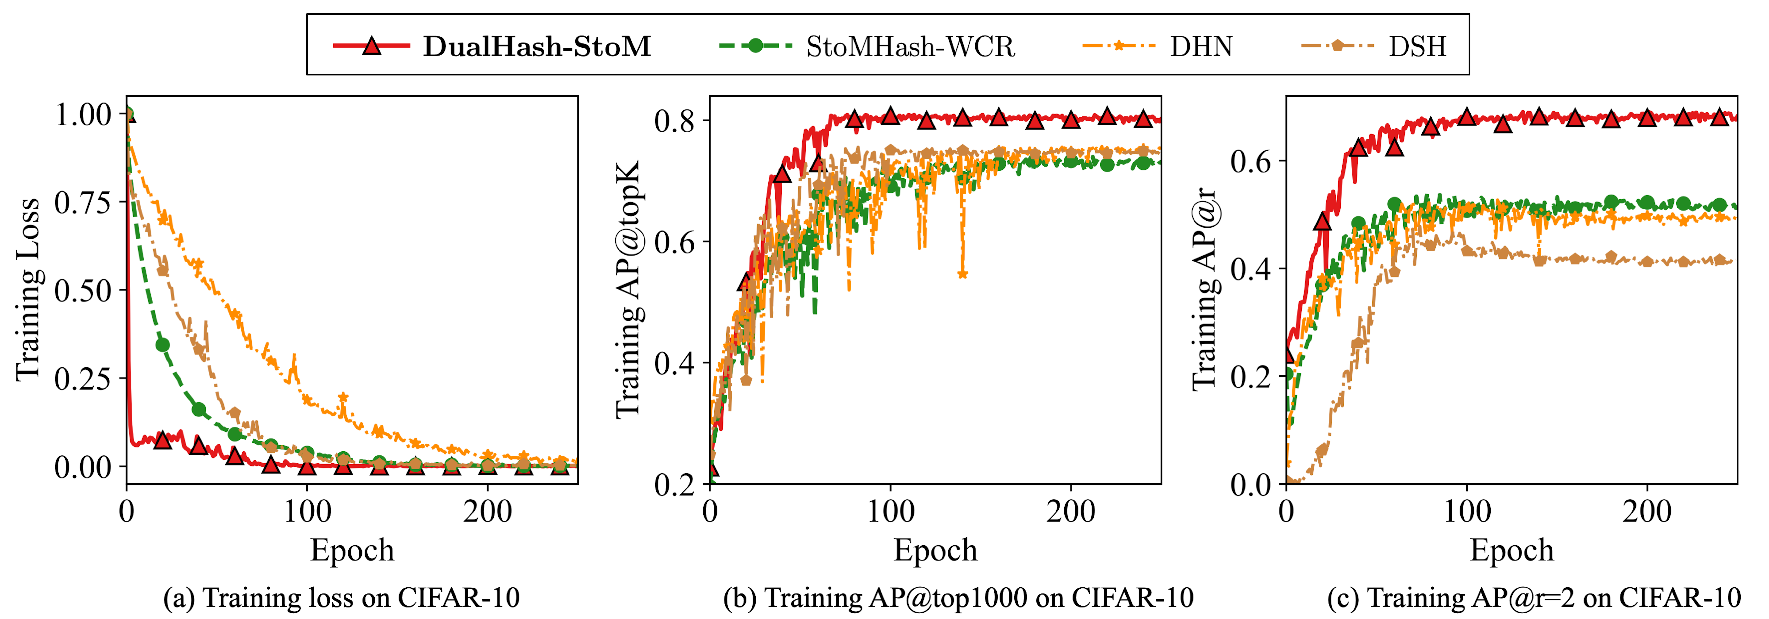
\includegraphics[width=0.95\textwidth]{results_images/ex3_training_cifar10.pdf}
    \caption{Training performance comparison of DualHash-StoM and three baselines with 64-bit codes on the CIFAR-10 dataset.}
    \label{Fig: Comparison of training performance of Different Methods on CIFAR-10}
\end{figure}
\begin{figure}[t]
    \centering
    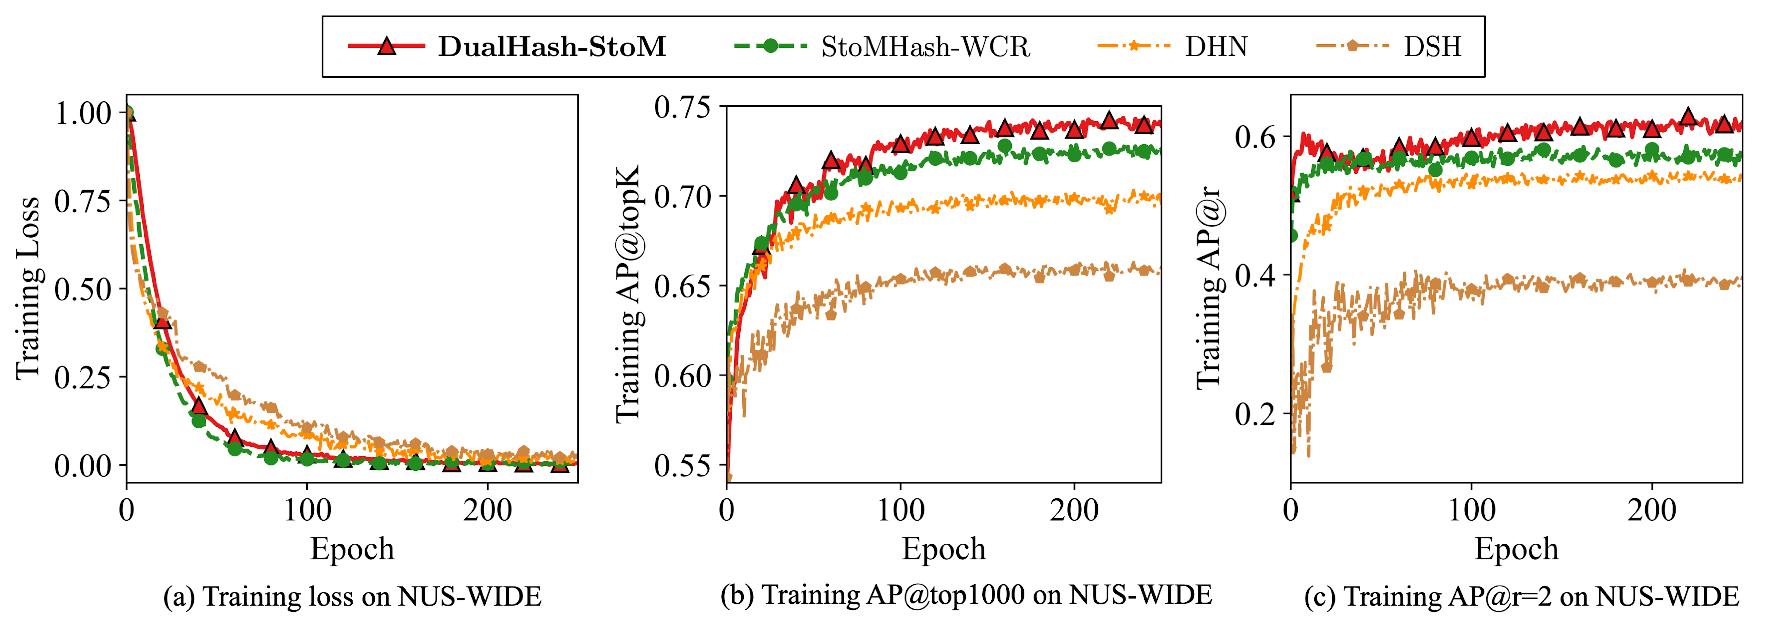
\includegraphics[width=0.95\textwidth]{results_images/ex3_training_nuswide.pdf}
    \caption{Training performance comparison of DualHash-StoM and three baselines with 64-bit codes on the NUS-WIDE dataset.}
    \label{Fig: Comparison of training performance of Different Methods on NUS-WIDE}
\end{figure}

\begin{table}[htbp]
    \centering
    \caption{Retrieval performance comparison of DualHash-StoM and three baselines with 64-bit codes on CIFAR-10 and NUS-WIDE datasets.}
    \label{tab:performance_comparison_64bits}
    \resizebox{0.93\textwidth}{!}{
    \begin{tabular*}{1\textwidth}{@{\extracolsep{\fill}}lcccccc@{}}
        \toprule 
        \multirow{2}{*}{Methods} & \multicolumn{3}{c}{CIFAR-10} & \multicolumn{3}{c}{NUS-WIDE} \\
        \cmidrule(lr){2-4} \cmidrule(lr){5-7}
         & mAP@All & P@r=2 & Time\textsuperscript{*} & mAP@5000 & P@r=2 & Time\textsuperscript{*} \\
        \midrule 
        DSH \cite{liuDeepSupervisedHashing} & 0.8010 & 0.4401 & 7.38 & 0.6634 & 0.4004 & 21.14 \\
        DHN \cite{zhuDeepHashingNetwork2016} & 0.8051 & 0.5272 & \textbf{6.74} & 0.7042 & 0.5432 & \textbf{16.47} \\
        StoMHash-WCR & 0.7773 & 0.5402 & 7.04 & 0.7225 & 0.5857 & 16.69 \\
        \textbf{DualHash-StoM} & \textbf{0.8539} & \textbf{0.6872} & 6.86 & \textbf{0.7448} & \textbf{0.6548} & 16.83 \\
        \bottomrule
    \end{tabular*}}
    
    \parbox{0.93\textwidth}{\footnotesize
    \textsuperscript{*}Training time per epoch (seconds). \textbf{Bold} values indicate the best results.
    }
\end{table}

\paragraph{Retrieval performance in Hamming space}
We report mAP, P@r=2, and the average time per training epoch on CIFAR-10 and NUS-WIDE, all
with 64-bit codes, for different methods in
Table~\ref{tab:performance_comparison_64bits}. The results highlight the superior retrieval
accuracy of DualHash-StoM compared to the baseline methods.

Specifically, on the CIFAR-10 dataset, DualHash-StoM achieves 9.9\% and 27.2\%
improvements over StoMHash-WCR in mAP@All and P@r=2, respectively. Similarly, on the
NUS-WIDE dataset, DualHash-StoM outperforms StoMHash-WCR with a 3.1\% improvement
in mAP@5000 and an 11.8\% improvement in P@r=2. Computationally, DualHash-StoM shows comparable efficiency to baselines such as DHN
(e.g., 6.86s vs. 6.74s on CIFAR-10 and 16.83s vs. 16.47s
on NUS-WIDE). This marginal time increase is justified by the substantial performance gains.
Furthermore, \Cref{fig:ex3_testing_2datasets} displays P@topK results and PR curves
with 64-bit codes on CIFAR-10 and NUS-WIDE. DualHash-StoM consistently outperforms all
comparison methods by large margins in P@topK. For PR curves, DualHash-StoM
demonstrates superior performance at lower recall levels, making it especially well-suited
for precision-critical image retrieval systems.

\begin{figure}[htbp]
    \centering
    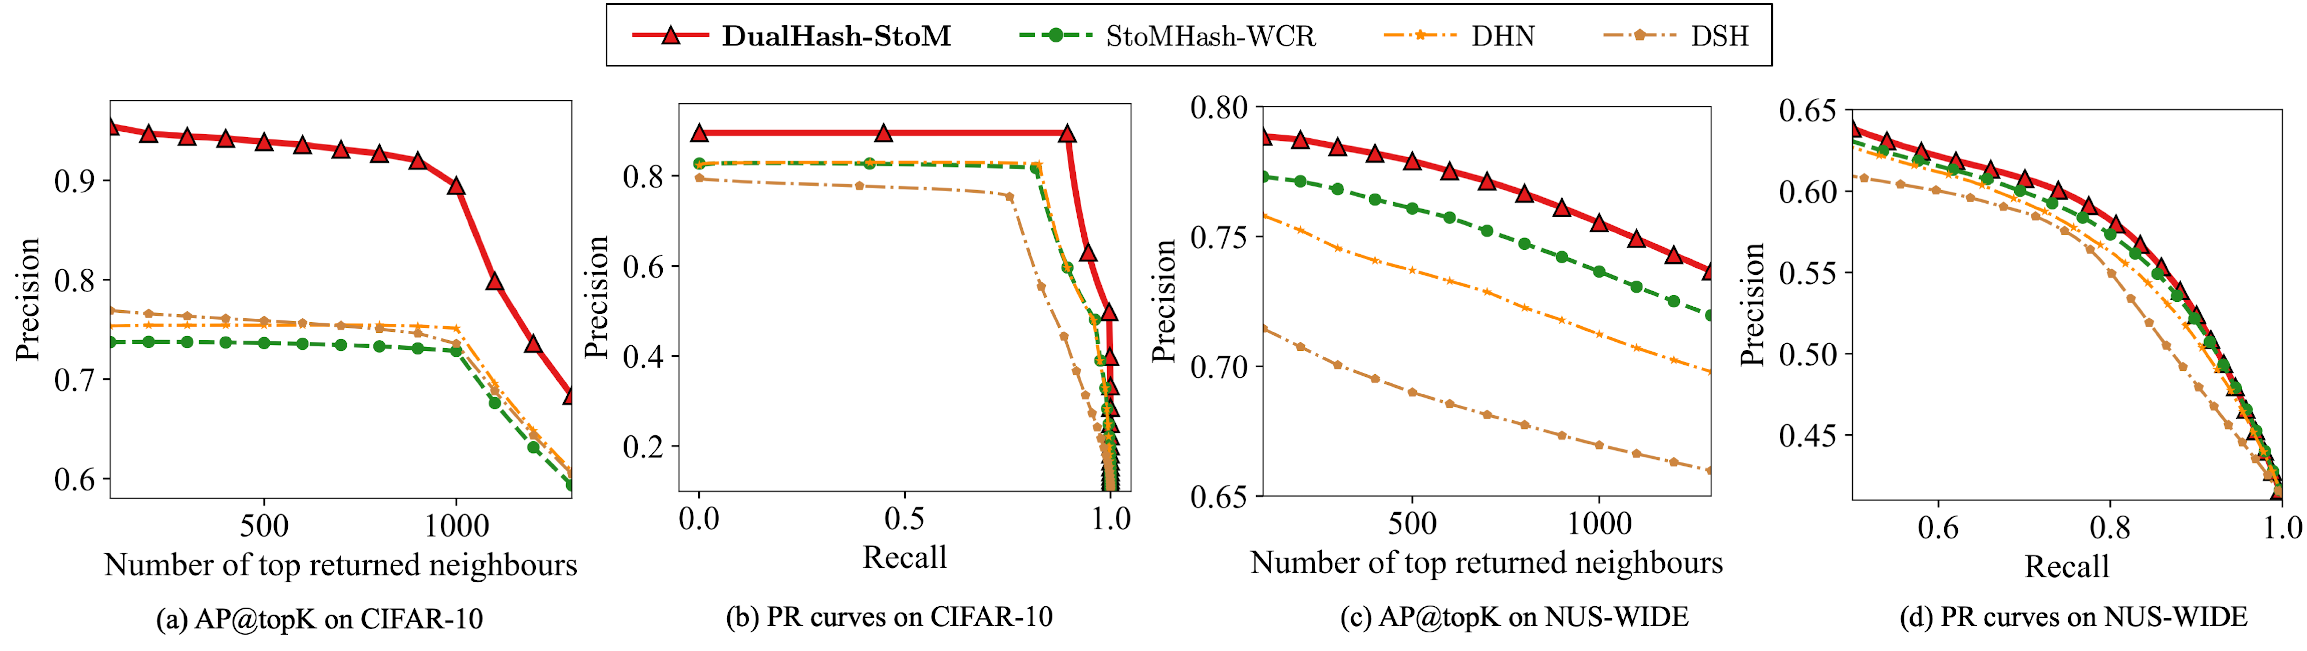
\includegraphics[width=0.95\textwidth]{results_images/ex3_testing_2datasets.pdf}
    \caption{Retrieval performance comparison of DualHash-StoM and three baselines with 64-bit codes on CIFAR-10 and NUS-WIDE datasets. (a), (c): P@topK results; (b), (d): PR curves.}
    \label{fig:ex3_testing_2datasets}
\end{figure}

% \end{document}
   % → E, F

\end{document}
